\documentclass[ 11pt
				,ngerman 
				,headsepline
				,headings=small
				,numbers=noenddot % Kein "." hinter der letzten Kapitelnummer --> 2.1 statt 2.1.
				,draft=false
				,BCOR=0mm % Wert für die Bindung 
				,DIV=12 % Wert für die größe des Textblocks
				,captions=tableheading
				,paper=a4
				,abstracton
				,twoside % Erlaubt beidseitigen Druck
                ]{scrreprt}
% Wählt den passenden Offset und Margin für das Deckblatt und wählt ein passenden Seitenlayout
\makeatletter
\newlength\offsetCoverPage
\newlength\marginCoverPage
\newcount\onesideprint
\if@twoside
\usepackage[a4paper, left=2.6cm, right=2.9cm, top=3.7cm, bottom=3.8cm]{geometry}
\offsetCoverPage=0.0cm
\marginCoverPage=0.25cm
\onesideprint=0
\else
\usepackage[a4paper, left=2.75cm, right=2.75cm, top=3.7cm, bottom=3.8cm]{geometry}
\offsetCoverPage=-0.10cm
\marginCoverPage=0cm
\onesideprint=1
\fi
\makeatother


%-----------------------------------------------------------------------------
% Größeninformationen:
% mit den gewählten Einstellungen beträgt die Textbreite (und damit auch die
% sinnvolle Bildbreite) ca. 158 mm
% Die Texthöhe beträgt etwa 215.0 mm, eine vollseitige Grafik sollte daher 
% maximal 200 mm hoch sein, halbseitige Grafiken entsprechend etwa 90 mm um
% genügend Raum für ein zweites Bild mit Bildunterschrift oder alternativ 
% Fließtext zu bieten
%-----------------------------------------------------------------------------

%-----------------------------------------------------------------------------
% Basispackete
%-----------------------------------------------------------------------------
\usepackage[utf8]{inputenc} 
%\usepackage[english]{babel} %Für einen englischen Text kommentiere die nächste Zeile und entferne den Kommentar dieser Zeile
\usepackage[ngerman]{babel} 
\usepackage{ifpdf} 
\usepackage{blindtext} % Um den lorem ipsum Text zu erzeugen
                      
%-----------------------------------------------------------------------------
% Schrifteinstellungen
%-----------------------------------------------------------------------------
\usepackage{fourier} %PDF-compatible font "Utopia". There exists a free look-alike: Heuristica
\makeatletter % No warnings because of a replaced font
  \let\@font@info\@gobble
  \let\@font@warning\@gobble
\makeatother
\usepackage[official]{eurosym} % Eurosymbol
\DeclareUnicodeCharacter{20AC}{\euro} % The normale euro symbol via [Alt Gr][€] is replaced by a high quality one
\renewcommand{\caplabelfont}{\bfseries} % Fig. and Tab. are bold
\usepackage{color}
\definecolor{ercred}{RGB}{229,48,39}
\usepackage{setspace} % Change Linespread
\onehalfspacing % Linespread 1.5
\setlength\parskip{\medskipamount} % Small linespread between two paragraphs
\setlength\parindent{0pt} % No indentation in the first line of a new paragraph
\AtBeginDocument{
  \renewcommand{\labelitemi}{\(\triangleright\)} % re-definition of the bullet-points
  \renewcommand{\labelitemii}{\(\bullet\)}}

%-----------------------------------------------------------------------------
% Seitenlayout
%-----------------------------------------------------------------------------
\usepackage[automark, autooneside=false]{scrlayer-scrpage}
% Für eine genauere Erklärung lies scrguide.pdf, ca. Seite 240
\automark[chapter]{chapter}
\automark*[section]{}
\interfootnotelinepenalty=10000 % Fußnoten nicht über zwei Seiten verteilen

%Kopfzeile einseitiger Druck
\ifnum\onesideprint=1
\pagestyle{scrheadings}
 \clearscrheadfoot
 \automark{chapter}
 \renewcommand\sectionmark[1]{\markright{\MakeMarkcase {\thesection\hskip .5em\relax#1}}} 
 \rohead{\ifnum\expandafter\pdfstrcmp\botmark=0 \rightmark\else\leftmark{} --- \rightmark\fi}
\ihead{\leftmark}
\ohead{\rightmark}
\cfoot{\pagemark}
\fi
%-----------------------------------------------------------------------------
% Tabellen
%-----------------------------------------------------------------------------
\usepackage{longtable}
\usepackage{multirow}
\usepackage{booktabs} % Erstelle besser aussehende Tabellen, nutze \toprule, \midrule, \bottomrule für horizontale Linien
\usepackage[point]{rccol} % Werte werden über das Kommata ausgerichtet
\usepackage[table,xcdraw]{xcolor}

%-----------------------------------------------------------------------------
% Abbildungen
%-----------------------------------------------------------------------------
\usepackage{subfigure}
\usepackage{float}
% Reduzierung der Anzahl von "Float-Only"-Seiten
\renewcommand{\topfraction}{0.85}
\renewcommand{\textfraction}{0.1}
\renewcommand{\floatpagefraction}{0.75}

%-----------------------------------------------------------------------------
% Mathematik
%-----------------------------------------------------------------------------
\usepackage{amsmath}
\usepackage{amssymb}
\usepackage{array}
\usepackage[cdot,thickqspace,squaren,textstyle]{SIunits} % SI-Einheiten können mit Namen eingegeben werden
\usepackage{nicefrac}


%-----------------------------------------------------------------------------
% Verweise und Zitate
%-----------------------------------------------------------------------------
\usepackage{varioref}
\usepackage[numbers, square]{natbib}
\usepackage{bibunits}

%-----------------------------------------------------------------------------
% PDF-Setup
%-----------------------------------------------------------------------------
\ifpdf
	%wir benutzen PDFLaTeX
	\usepackage[pdftex]{graphicx} 
	\pdfimageresolution=100
	\pdfminorversion=7
	\pdfcompresslevel=9
	\usepackage[pdftex,
		urlcolor=blue,
		linktoc=all,
		colorlinks=true,
		linkcolor=black,
		citecolor=black,
		pdfview=FitH,
		pdfstartview=FitH,
		plainpages=false]{hyperref}
	\hypersetup{
		pdfauthor={Your Name here},
        pdftitle={Name of your thesis},
        pdfsubject={},
        pdfkeywords={several helpful keywords},
        pdfproducer={LaTeX with hyperref},
        pdfcreator={pdflatex}}
    \usepackage[figure,figure*]{hypcap}
\else
	%DVI oder PS Ausgabe
	\usepackage{graphicx} 
\fi

%-----------------------------------------------------------------------------
% JETZT GEHTS LOS!
%-----------------------------------------------------------------------------
\begin{document}
\pagestyle{empty}
\newcounter{Hilfszaehler}

%-----------------------------------------------------------------------------
% Deckblatt
%-----------------------------------------------------------------------------
\begin{titlepage}
\begin{addmargin}{\offsetCoverPage} 
%TODO Um das RWTH-Logo zu benutzen, musst du das Formblatt RWTH-Logo Deutsch aus der Datei Formulare.txt
%TODO ausfüllen und es dem ZPA schicken!

%-----------------------------------------------------------------------------
% Platzierung der Kopfzeile(Nummer und Logo)
%-----------------------------------------------------------------------------
\setlength{\unitlength}{1cm}
\begin{picture}(0,0)
\put(7.977,0.68){
\includegraphics[width = 0.5\textwidth]{Pictures/rwth_eerc_rgb_ohne_Schutzraum}}
%TODO Ändere die Nummer deiner Arbeit, und wenn noetig die Bezeichnung(BA, MA, PA)
%TODO Die Abkürzungen sind Deutsch, auch wenn die Arbeit in Englisch verfasst wird
\put(0,1.32){\fontfamily{phv}\selectfont\huge{BA tba}}
\end{picture}
\end{addmargin}
%-----------------------------------------------------------------------------
% Titel deiner Arbeit
%-----------------------------------------------------------------------------
\addvspace{2.6cm}
%TODO Formaenderung des Titels
\begin{addmargin}[\marginCoverPage]{0cm}
\begin{center}
{\fontfamily{phv}\selectfont\huge Bachelorarbeit} 
\end{center}

{\Large \par}
\addvspace{1.5cm}
\begin{center}
%TODO Wenn du ein "Sperrvermerk" für deine Arbeit brauchst, entferne den Kommentar in der naechsten Zeile
%\textbf{{\color{ercred}\fontfamily{phv}\selectfont{\huge Sperrvermerk}}}\\

%TODO  Der Englische Titel deiner Arbeit wird nach dem "\huge" in der naechsten Zeile geaendert
\textbf{\fontfamily{phv}\selectfont{\huge Design einer Abschlussarbeit}}
\end{center}

%\addvspace{1.5cm}
%\begin{center}
%TODO Falls der deutsche Name noch noetig ist, kommt er in die naechste Zeile
%{\fontfamily{phv}\selectfont Design of a Master's thesis}
%\end{center}

%-----------------------------------------------------------------------------
% Namen, Daten
%-----------------------------------------------------------------------------
\vfill
\begin{center}
\begingroup
\fontfamily{phv}\selectfont
%TODO Bitte aendere das Datum deiner Abgabe
Aachen, Mai 2019 \\
\addvspace{0.5cm}
%TODO Bitte aendere deinen Namen und Matrikelnummer in den naechsten beiden Zeilen
\textbf{Jonas Baumgärtner} \\
Matrikelnummer: 330575 \\
\addvspace{0.5cm}
%TODO Deine Betreuer. Achte auf die richtige Schreibweise des Titels.
Betreuer:\\
Sebastian Remy, M. Sc. \\
Univ.-Prof. Dr.-Ing. Dirk Müller \\
\addvspace{0.5cm}
%TODO  Eingabe der richtigen Anschrift des Instituts.
Diese Arbeit wurde vorgelegt am:\\
E.ON Energy Research Center | ERC \\
Institute for Energy Efficient Buildings and Indoor Climate | EBC\\
(Lehrstuhl für Gebäude- und Raumklimatechnik)\\
Mathieustraße 10, 52074 Aachen\\
\endgroup
\end{center}
\end{addmargin}
\end{titlepage}



%-----------------------------------------------------------------------------
% Setup von speziellen Seiten(Abbildungsverzeichnis, Nomenklatur etc.
%-----------------------------------------------------------------------------
\cleardoublepage
\pagenumbering{Roman} % Romanische Nummerierung
%-----------------------------------------------------------------------------
% Englische und Deutsche Kurzfassung. Beide notwendig
%-----------------------------------------------------------------------------
\clearpage
\refstepcounter{Hilfszaehler}
\renewcommand\abstractname{Kurzfassung}
\begin{abstract}
Überall dieselbe alte Leier. Das Layout ist fertig, der Text lässt auf sich warten. Damit das Layout nun nicht nackt im Raume steht und sich klein und leer vorkommt, springe ich ein: der Blindtext. Genau zu diesem Zwecke erschaffen, immer im Schatten meines großen Bruders »Lorem Ipsum«, freue ich mich jedes Mal, wenn Sie ein paar Zeilen lesen. Denn esse est percipi - Sein ist wahrgenommen werden.

Und weil Sie nun schon die Güte haben, mich ein paar weitere Sätze lang zu begleiten, möchte ich diese Gelegenheit nutzen, Ihnen nicht nur als Lückenfüller zu dienen, sondern auf etwas hinzuweisen, das es ebenso verdient wahrgenommen zu werden: Webstandards nämlich. Sehen Sie, Webstandards sind das Regelwerk, auf dem Webseiten aufbauen. So gibt es Regeln für HTML, CSS, JavaScript oder auch XML; Worte, die Sie vielleicht schon einmal von Ihrem Entwickler gehört haben. Diese Standards sorgen dafür, dass alle Beteiligten aus einer Webseite den größten Nutzen ziehen.

Im Gegensatz zu früheren Webseiten müssen wir zum Beispiel nicht mehr zwei verschiedene Webseiten für den Internet Explorer und einen anderen Browser programmieren. Es reicht eine Seite, die - richtig angelegt - sowohl auf verschiedenen Browsern im Netz funktioniert, aber ebenso gut für den Ausdruck oder die Darstellung auf einem Handy geeignet ist. Wohlgemerkt: Eine Seite für alle Formate. Was für eine Erleichterung. Standards sparen Zeit bei den Entwicklungskosten und sorgen dafür, dass sich Webseiten später leichter pflegen lassen. Natürlich nur dann, wenn sich alle an diese Standards halten. Das gilt für Browser wie Firefox, Opera, Safari und den Internet Explorer ebenso wie für die Darstellung in Handys. Und was können Sie für Standards tun? Fordern Sie von Ihren Designern und Programmieren einfach standardkonforme Webseiten. Ihr Budget wird es Ihnen auf Dauer danken. Ebenso möchte ich Ihnen dafür danken, dass Sie mich bin zum Ende gelesen

This abstract has 300 words

\end{abstract}
\renewcommand{\abstractname}{Abstract}
\begin{abstract}

 
\end{abstract}

%-----------------------------------------------------------------------------
% Inhaltsverzeichnis
%-----------------------------------------------------------------------------
\pagestyle{plain.scrheadings}
\setcounter{secnumdepth}{2}
\setcounter{tocdepth}{2}
\tableofcontents

%-----------------------------------------------------------------------------
% Nomenklatur
%-----------------------------------------------------------------------------
\clearpage
\refstepcounter{Hilfszaehler}
\addcontentsline{toc}{chapter}{Nomenklatur}
\chapter*{Nomenklatur}
\begin{onehalfspacing}
\begin{longtable}[h]{p{0.15\textwidth} p{0.65\textwidth} p{0.1\textwidth}}
		\caption*{\textbf{Formelzeichen und Einheiten}} \\
		\\
		\textbf{Symbol} & \textbf{Bedeutung} & \textbf{Einheit} \\ %\hline 
		\endhead
		\\
		\multicolumn{3}{c}{Fortsetzung auf der nächsten Seite} \\
		\endfoot
		\multicolumn{3}{c}{ } \\
		\endlastfoot
		
		$A$ & Fläche & \squaremetre\\
		$c_{p}$&spezifische Wärmekapazität bei konstantem Druck&\joule\per(\kilogram\usk\kelvin)\\
			$C$&Wärmekapazität&\watt\per\kilogram\\
		$H $ & Enthalpie & \joule\\		
		$\dot{H}$ & Enthalpiestrom & \joule\per\second\\
		$E$ & Exergie & \joule\\
		$e$ & spezifische Exergie & \joule\per\kilogram\\
		$\dot{m}$ & Massenstrom & \kilogram\per\second\\
		$p$ & Druck & \pascal\\
		$\dot{Q}$ & Wärmestrom & \watt\\
		$R$ & spezifische Gaskonstante & \joule\per(\kilogram\usk\kelvin)\\
		$S$ & Entropie & \joule\per\kelvin\\
		$\dot{S}$ & Entropiestrom & \watt\per\kelvin\\
		$T$ & Temperatur & \kelvin\\
		$t$ & Zeit & \second\\
		$U$ & innere Energie & \joule\\
		$U_{T}$ & Wärmedurchgangskoeffizient & \watt\per(\kilogram\usk\kelvin)\\
		$h$ & Wärmeübergangskoeffizient & \watt\per(\squaremetre\usk\kelvin)\\		
		$V$ & Volumen & \cubic\meter\\
		$\dot{V}$&Volumenstrom&\cubic\meter\per\second\\
		$\dot{W}$ & Leistung & \watt\\
		$Y$ & Wasserbeladung der Luft & \gram\per\kilogram\\
		
		
\end{longtable}

\begin{longtable}[h]{p{0.15\textwidth} p{0.65\textwidth} p{0.1\textwidth}}
		\caption*{\textbf{Griechische Formelzeichen}} \\
		\\
		\textbf{Symbol} & \textbf{Bedeutung} & \textbf{Einheit} \\ %\hline 
		\endhead
		\\
		\multicolumn{3}{c}{Fortsetzung auf der nächsten Seite} \\
		\endfoot
		\multicolumn{3}{c}{ } \\
		\endlastfoot
		
		$\eta_{C}$ & Carnot-Wirkungsgrad & ---\\
		$\kappa_{\mathrm{E}}$ & exergetische Aufwandszahl der Wärmeerzeugung & ---\\
		$\kappa_{\mathrm{T}}$ & exergetische Aufwandszahl des Wärmetransfers & ---\\
		$\Phi$ & thermische Leistung & \watt\\
		$\varrho$& Massendichte&\kilogrampercubicmetre\\
			$\sigma$&Temperaturspreizung&\kelvin\\
		$\vartheta $ & Temperatur  & \degreecelsius\\
		$\Delta\vartheta $ & Temperaturdifferenz  &\kelvin\\
		
\end{longtable}

\begin{longtable}[h]{p{0.15\textwidth} p{0.75\textwidth}}
		\caption*{\textbf{Indizes und Abkürzungen}} \\
		\\
		\textbf{Symbol} & \textbf{Bedeutung} \\ %\hline 
		\endhead
		\\
		\multicolumn{2}{c}{Fortsetzung auf der nächsten Seite} \\
		\endfoot
		\multicolumn{2}{c}{ } \\
		\endlastfoot
		
		0 & Referenzzustand (\emph{ambient dead state})\\
		A & Außen/Umgebung\\ 		
		CH & chemisch\\
		CV & Kontrollvolumen (\emph{control volume})\\
		DSC & Dynamische Differenzkalorimetrie (\emph{differential scanning calorimetry}) \\
		e & über die Systemgrenze (\emph{external})\\
		F & Volumenstrom\\	
		FW & Fassadenwärmeübertrager\\
		gen & erzeugt (\emph{generated})\\
		In & Eingang (\emph{input})\\
		KN & kinetisch\\
		KRM & Kapillarrohrmatte\\
		LabVIEW & Programmiersprache und Entwicklungsumgebung für die Messdatenerfassung der Firma National Instruments\\
		L & Luft\\
		LWS & Latentwärmespeicher\\	
		m & Mittelwert\\
			Ob&Oberfläche\\
		PCM & Latentwärmespeichermaterial (\emph{phase change material})\\
		PH & physikalisch\\
		PT & potentiell\\
		Q & auf einen Wärmestrom bezogen\\
		R & Rücklauf\\
		Reg& Speicherregeneration\\
		T & Temperatur\\
		$\Delta$ t & Zeitschritt der Länge $\Delta$ t\\
		t & technisch\\
		V & Vorlauf\\
		V & Verlust (Exergieanalyse)\\
		W&Wärmeträgermedium\\
		
\end{longtable}
\end{onehalfspacing}


%-----------------------------------------------------------------------------
% Abbildungsverzeichnis
%-----------------------------------------------------------------------------
\clearpage
\refstepcounter{Hilfszaehler}
\addcontentsline{toc}{chapter}{Abbildungsverzeichnis}
\listoffigures

%-----------------------------------------------------------------------------
% Tabellenverzeichnis
%-----------------------------------------------------------------------------
\clearpage
\refstepcounter{Hilfszaehler}
\addcontentsline{toc}{chapter}{Tabellenverzeichnis}
\listoftables

%-----------------------------------------------------------------------------
% Vorwort, kommentiere die Zeile wenn nicht nötig
%-----------------------------------------------------------------------------
\clearpage
\refstepcounter{Hilfszaehler}
\addcontentsline{toc}{chapter}{Vorwort}
%\newpage\thispagestyle{empty}~
\chapter*{Vorwort}



%-----------------------------------------------------------------------------
% Setup Normale Seiten(Neue Nummerierung)
%-----------------------------------------------------------------------------
\cleardoublepage
\clearpage
\pagenumbering{arabic}
\pagestyle{scrheadings}%\ihead{\leftmark}\chead{}\ohead{\rightmark}
\automark[chapter]{chapter}
\automark*[section]{}

%-----------------------------------------------------------------------------
% Füge hier deine Kapitel hinzu
%-----------------------------------------------------------------------------
\chapter{Einleitung}

\section{Motivation}
\label{sec:Sektion 11}
das ist die einleitung
\section{Aufgabenstellung}
\label{sec:Sektion 12}
das ist die aufgabenstellung
\chapter{Grundlagen}

Ziel dieser Arbeit ist die Ermittlung optimierter Gebäudeenergiesysteme für den deutschen Wohngebäudebestand.
Hierzu wurde in Kapitel \ref{sec:Sektion 21} der Bestand analysiert, um auf dieser Untersuchung aufbauend die nationale Wohngebäudesituation in einigen wenigen, repräsentativen Klassen abzubilden. 
Des Weiteren wurde in \ref{sec:Sektion 22} die historische Entwicklung der Gebäudehülle betrachtet. Daraus wurden Zeiträume der Baualtersklassen mit ähnlichen Baustoffen und Dämmdicken zusammengefasst. 
Zuletzt stellt Kapitel \ref{sec:Sektion 23} die Grundlagen der mathematischen Optimierung sowie das im Rahmen dieser Arbeit erweiterte Optimierungsprogramm vor. 

%Die Gebäudeklassen sollen für die Bestimmung der Gebäudeenergiesysteme mit dem Optimierungsprogramm benutzt werden. 
%Hieraus soll ein Vergleich zwischen Emissionsoptimum sowie Kostenoptimum gewonnen werden.

%Gebäudeenergiesysteme erklären?
%Was hat das überhaupt mit Grundlagen zu tuen, was ich da schreibe?
%Nehm ich in der Einleitung des Kapitels hier zuviel vorweg?
%Ist es okay, hier den Vergleich zu erwähnen? Evl. umschreiben
%Letzter Satz beschissen





\section{Deutscher Wohngebäudebestand}
\label{sec:Sektion 21}

Zunächst wurde der Wohngebäudebestand hinsichtlich Alter und Größe ausgewertet.
Als Daten wurden die Statistiken des Zensus2011, einer nationalen statistischen Erhebung von privaten Haushalten, betrachtet. 
Besagte Statistiken wurden in verschiedenen wissenschaftlichen Untersuchungen des Institut für Wohnen und Umwelt GmbH (IWU) ausgewertet und evaluiert.
Weiterhin wurde für die gebäudetypischen Kennwerte die Typgebäude des europaweiten Projekts \glqq Typology Approach for Building Stock Energy Assessment\grqq\,(TABULA) berücksichtigt. Diese Daten wurden ebenfalls vom IWU erhoben und berechnet.
%Tabula evtl erst im nächsten Kapitel erläutern, da bei der statistischen Betrachtung fast nur Zensus/IWU Daten betrachtet werden

Nach den 2011 veröffentlichten Zensus Daten besteht der deutsche Wohngebäudebestand aus rund 18.368.000 Gebäuden mit 39.432.000 Wohnungen \cite{.2015}.
Wie in Abbildung \ref{fig: Abbildung211} zu erkennen ist, prägt den deutschen Wohngebäudebestand einen Boom in der Nachkriegszeit. 
So wurden in den Jahren von 1949 bis 1978 etwa 7,2 Millionen Häuser errichtet. Diese Klasse alleine macht \mbox{38 \%} der deutschen Wohngebäude aus. 
Mit circa 2,7 Millionen Gebäuden und einem Anteil von etwa \mbox{14 \%} bilden die vor 1919 fertiggestellten Wohnobjekte den zweitgrößten Anteil, sowie die Häuser mit Baualter zwischen 1919 und 1948 mit knapp \mbox{12 \%} die drittgrößte Gruppe.
Folglich sind knapp zwei Drittel der deutschen Wohngebäude vor 1978 erbaut worden.
Eine weitere relevante Klasse beschreiben mit fast \mbox{10 \%} die von 1979 bis 1986 geschaffenen Wohnbauten. 
Zusammen mit den drei Klassen \mbox{1987 - 1990,} \mbox{1991 - 1995} und \mbox{1996 - 2000} werden  durch diese vier Gruppen mehr als ein Viertel des Wohngebäudebestandes in Deutschland abgebildet.
Im Gegensatz zu den zuvor genannten Gruppen stellen die nach der Jahrtausendwende konstruierten Häuser mit unter \mbox{10 \%} und nur 1,6 Millionen Häusern einen relativ kleinen Anteil des nationalen Bestandes dar. 

Es sei noch zu erwähnen, dass in dieser Betrachtung den Mikrozensus-Klassen gefolgt wurde. 
Diese sind explizit keine gleich langen Zeitintervalle, sondern \glqq orientieren sich an historischen Einschnitten, den Zeitpunkten statistischer Erhebungen und den Veränderungen der wärmetechnisch relevanten Bauvorschriften\grqq \cite{.2015}. 
So beschreibt beispielsweise das relativ kurze Zeitintervall von 1979 bis 1983 den Zeitraum zwischen erster und zweiter Wärmeschutzverordnung, auf welche in Kapitel \ref{sec:Sektion 22} noch näher eingegangen wird.

\begin{figure}[H]
	\centering
		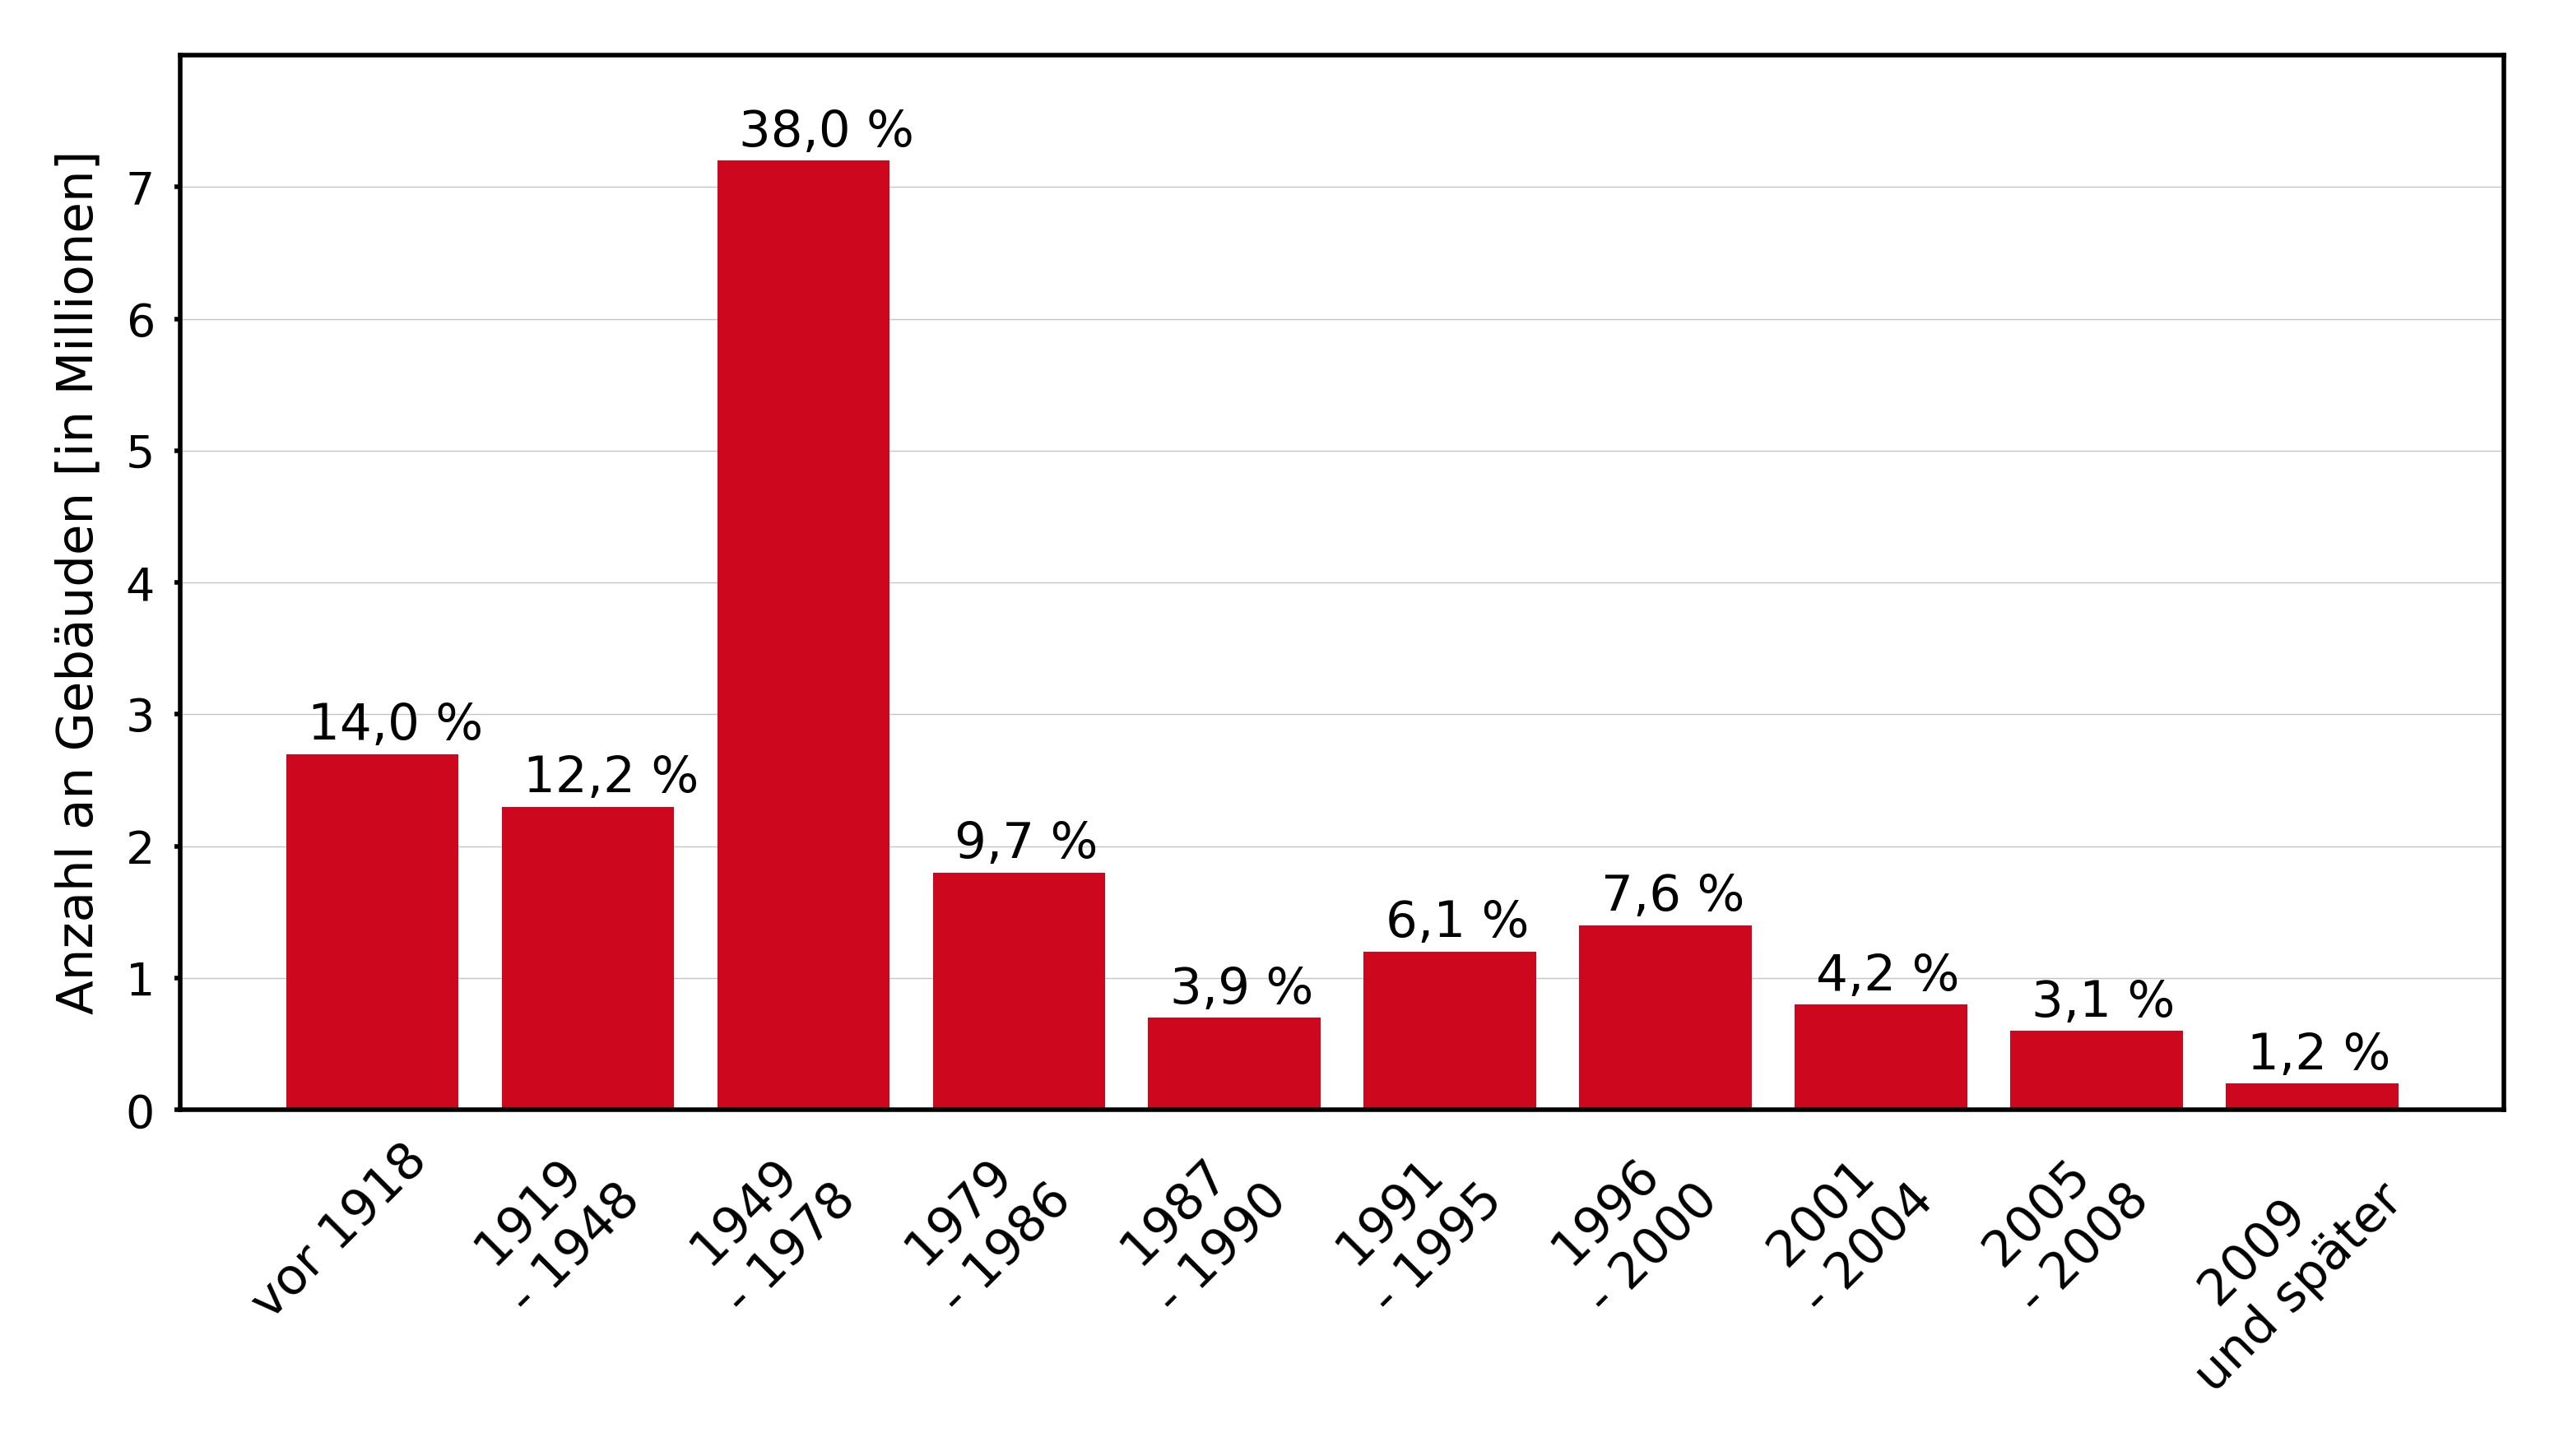
\includegraphics{Pictures/GebaeudeAlterDiagramm.jpg}
	\caption{errichtete Wohngebäude nach Mikrozensus-Klassen sowie deren Anteil am Gebäudebestand\cite{StatistischeAmterdesBundesundderLander.2014}}
	\label{fig: Abbildung211} 
\end{figure}
%Zwanzig Jahre Klassen vorstellen?

Eine weitere Unterteilung des Wohngebäudebestandes erhält man bei der Betrachtung der Anzahl an Wohneinheiten im Gebäude. 
Hierbei setzt sich der Bestand zu zwei Dritteln aus Wohngebäuden mit nur einer Wohnung zusammen. 
Weitere \mbox{17 \%} bilden Gebäude mit zwei Wohnungen und die Gebäudeklasse mit \mbox{3 - 6 Wohnungen} ist mit \mbox{12 \%} vertreten. 
Die größeren Gebäude mit \mbox{7 - 12 Wohnungen} sowie mit 13 und mehr Wohnungen sind anteilig am Gebäudebestand mit jeweils \mbox{5 \%} und \mbox{1 \%} relativ kleine Gruppen. 
Allerdings gelten letztere nur bei einer Gebäudebetrachtung als weniger relevant, da sie bei einer Anschauung der Wohneinheiten logischerweise mit größeren Faktoren im Vergleich zu Einfamilienhäusern eingehen. \cite{StatistischeAmterdesBundesundderLander.2014b}

In Abbildung \ref{fig: Abbildung212} sind die Anzahl der Wohneinheiten für die drei Baualtersklassen älter als 1978, \mbox{1979 - 1994} und \mbox{1995 - 2009} sowie deren Anteil an allen Wohneinheiten bis Baujahr 2009 des Gebäudebestandes dargestellt. 
In Anlehnung an den vorherigen Abschnitt werden Gebäude mit bis zu 2 Wohnungen als Ein- und Zweifamilienhäuser zusammengefasst und nach der englischen Bezeichnung \glqq single family home\grqq\,mit SFH abgekürzt. 
Wohngebäude mit 3 oder mehr Wohnungen werden als Mehrfamilienhäuser mit der Abkürzung MFH für \glqq multy family home\grqq\,gebündelt. 

Auffallend ist wiederum der enorme Anteil der Gebäude mit Baualter älter als 1978. 
Hier zählen die Mehrfamilienhäusern mit 14,8 Millionen Wohnungen und einem Anteil aller bis 2009 errichteten Wohneinheiten von \mbox{38 \%} zur größten Gruppe. 
Mit 12,5 Millionen Wohnungen und einem Anteil von 32\,\% entfällt die zweitgrößte Klasse auf die Einfamilienhäuser mit Baujahr älter 1978.
Ähnlich wie zuvor bei der Gebäudebetrachtung wurden somit auch mehr als zwei Drittel aller Wohnungen vor 1978 erbaut.

\begin{figure}[H]
	\centering
		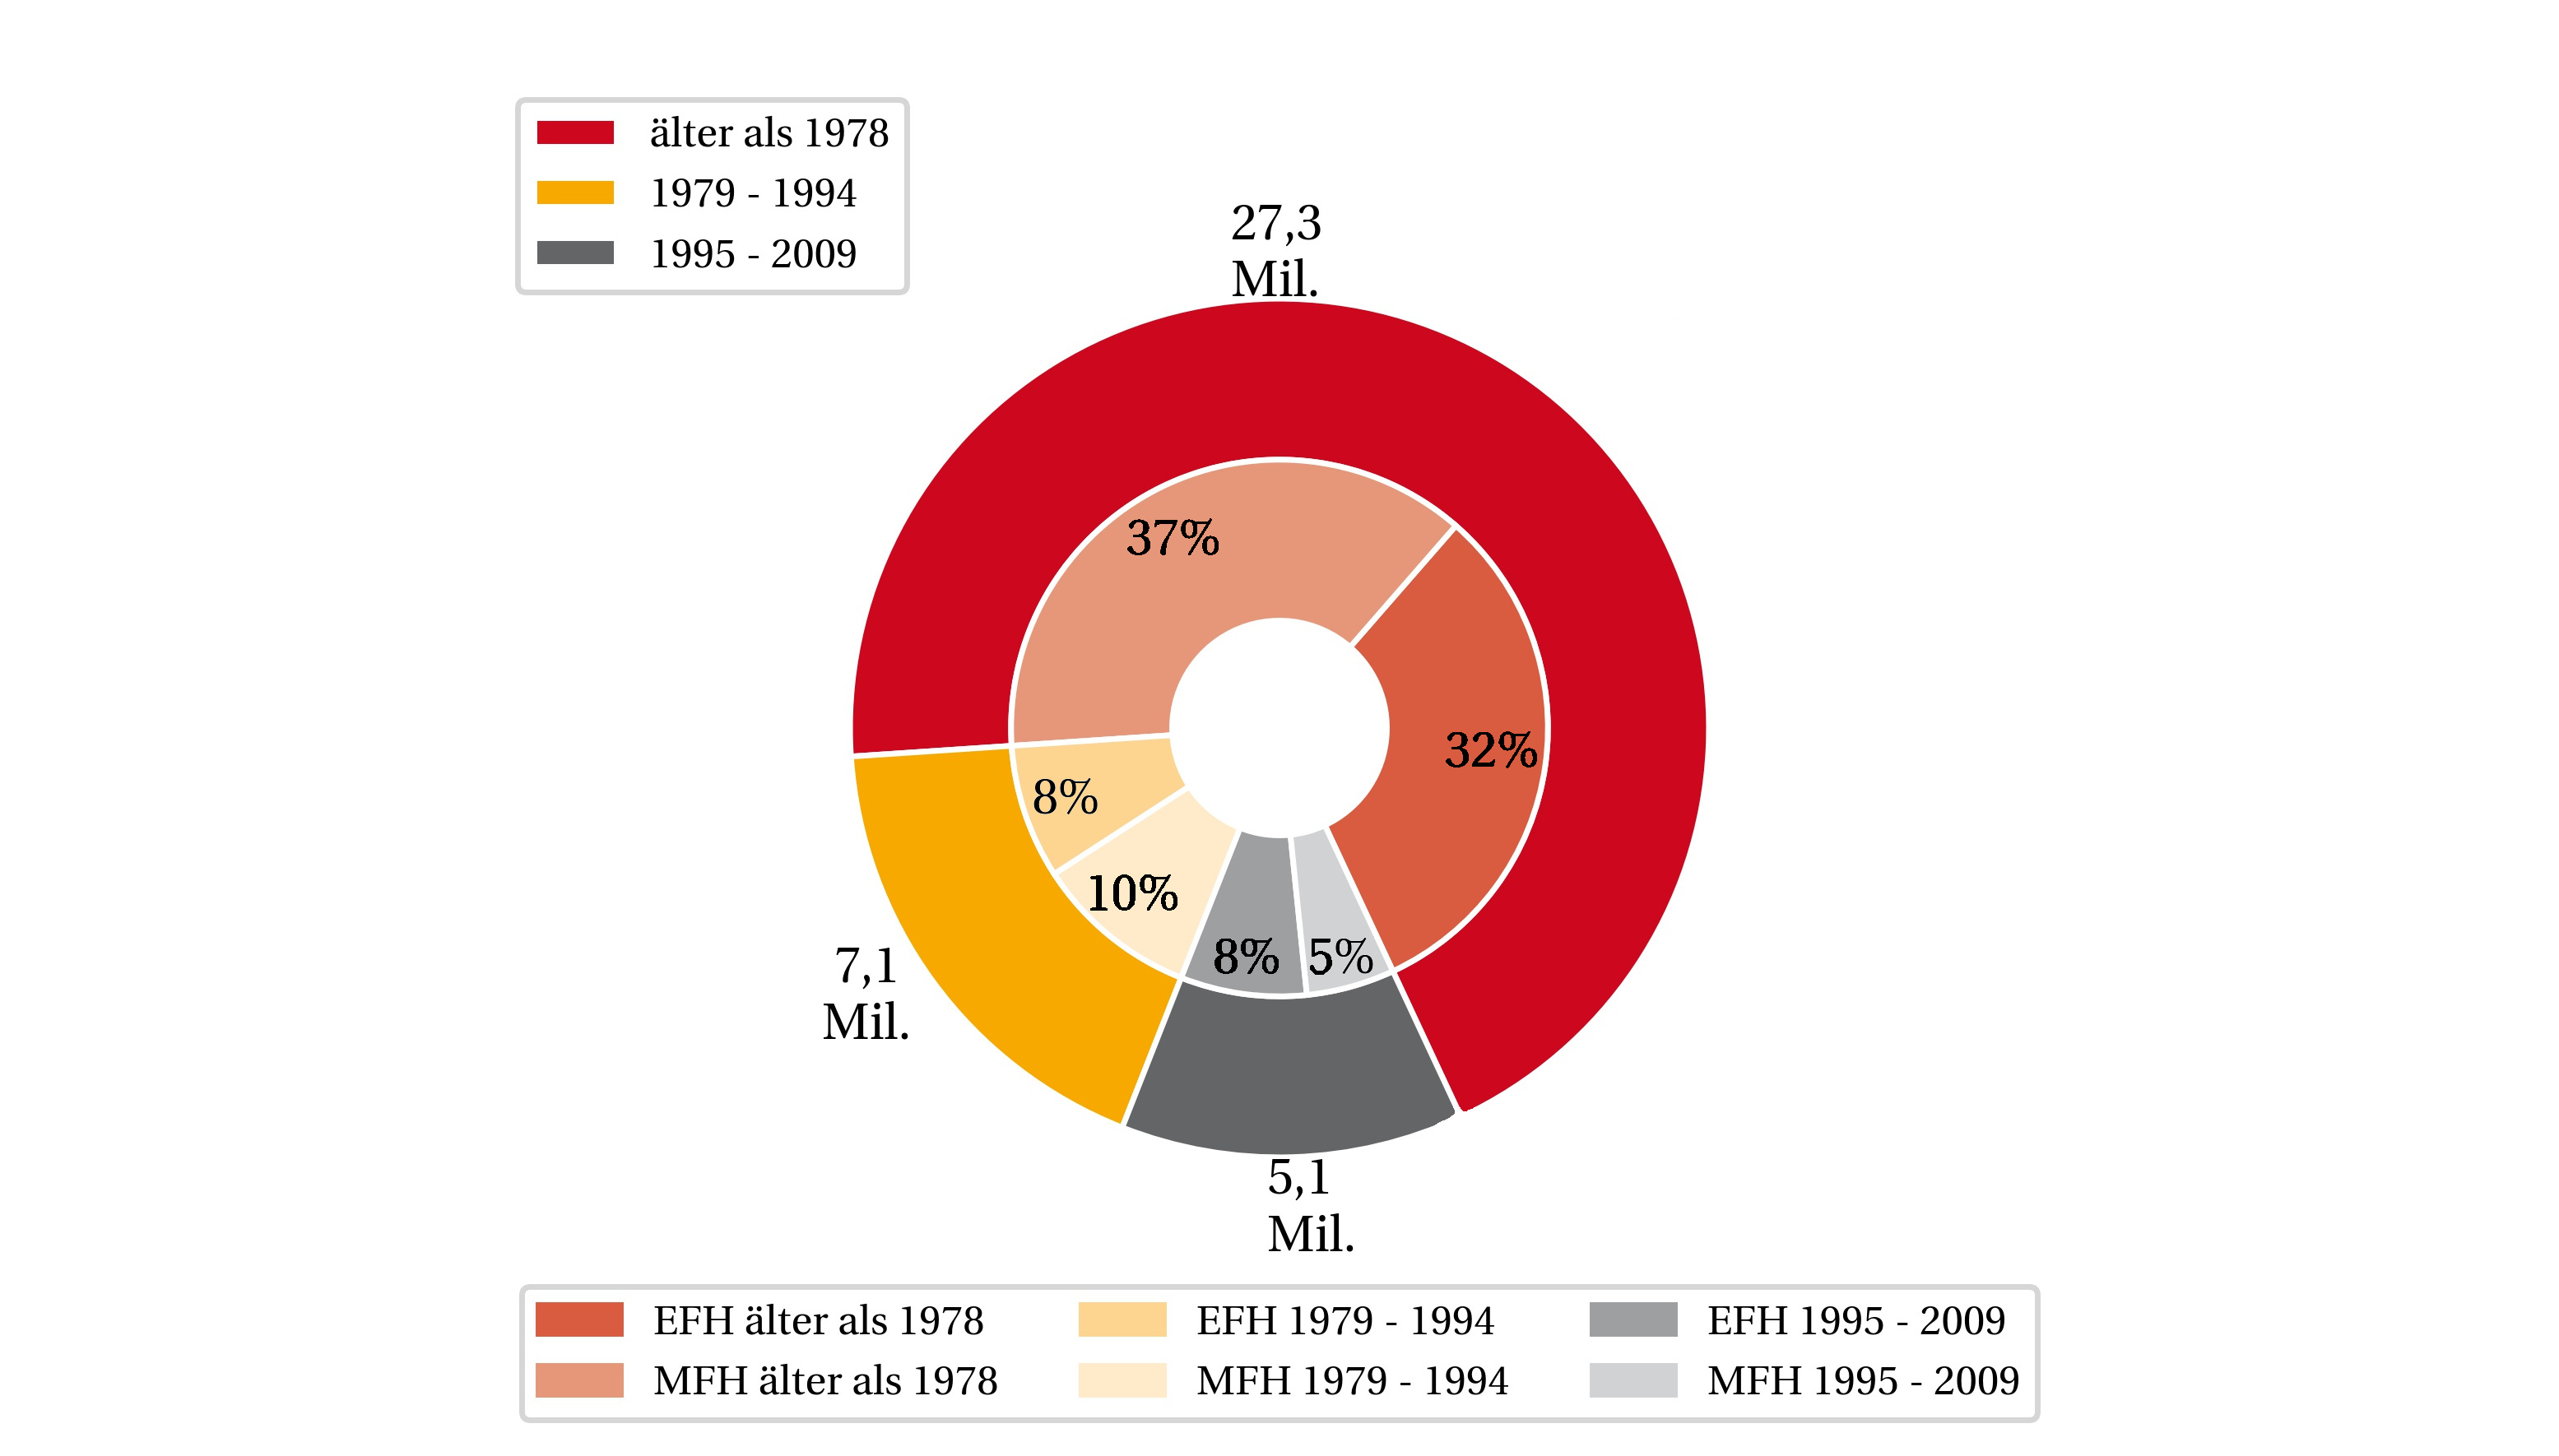
\includegraphics{Pictures/GebaeudeGroesse.jpg}
	\caption{Anzahl an Wohneinheiten bei Einfamilienhäuser (SFH) und Mehrfamilienhäuser (MFH) \cite{StatistischeAmterdesBundesundderLander.2014b}}
	\label{fig: Abbildung212} 
\end{figure}

Zusammenfassend lassen sich folgende Punkte bei der statistischen Betrachtung des deutschen Gebäudebestandes festhalten:

\begin{itemize}
	\item $\nicefrac{2}{3}$ aller Gebäude und Wohnungen des Bestandes wurden vor der 1. Wärmeschutzverordnung 1978 errichtet.
	\item Ein- und Zweifamilienhäuser stellen mit 87\,\% den größten Anteil der Gebäude dar. %Das hab ich vorher nicht erläutert
	\item Bei einer Betrachtung der Wohneinheiten halbiert sich der Bestand in Gebäude mit einer oder zwei Wohnungen (47\,\%) und drei oder mehr Wohnungen (53\,\%).
	\item Gebäude, die nach der Jahrtausendwende gebaut wurden, bilden keinen großen Anteil des Bestandes.
\end{itemize}

%Wohnobjekte?
%Zensus näher erläutern?
%Typgebäude näher beschreiben?
%Auf Wohnfläche eingehen?






\section{Historische Entwicklung der Gebäudehülle}
\label{sec:Sektion 22}

Nachdem im vorherigen Kapitel der Gebäudebestand nach Alter und Größe beschrieben wurde, werden nun die zu den jeweiligen Gebäudealtern zugehörigen Baustoffe und Dämmeigenschaften vorgestellt. 
Hierzu wird zwischen der Isolierung verschiedener Gebäudebauteilen unterschieden. 
Neben Möglichkeiten zur Dämmung des Daches beziehungsweise der obersten Geschossdecke und der Außenwand werden zudem die Dämmung des Bodens betrachtet.
Weiterhin wird auf den Verglasungsstandard verschiedener Epochen eingegangen
%Warum Dach und oberste Geschossdecke zusammengefasst werden kurz erklären?

Ein wichtiger Kennwert zur energetischen Bewertung eines Gebäudes und einzelner Gebäudekomponenten beschreibt der U-Wert.
Hierbei handelt es sich um den Wärmeübergangskoeffizienten, welcher den Wärmestrom durch 1\,m² Bauteilfläche bei 1\,Kelvin Temperaturdifferenz beschreibt. 
Berechnet wird dieser als Kehrwert des Wärmedurchgangswiderstand \(R_T\). 
Der U-Wert ist definiert als
\begin{equation}
\label{eq:Gleichung221}
U = \frac{1}{R_T}  \ \ \ \ \ \ \ \text{in} \ \ W/(m^2 \cdot K)
\end{equation}
wobei mit
\begin{equation}
\label{eq:Gleichung222}
R_T = \sum \limits_{i} \frac{d_i}{\lambda_i}	
\end{equation}				%Muss ich da innere, äußere Schicht unterscheiden?
der Wärmedurchgangswiderstand als Verhältnis der Dämmstoffdicke \(d_i\) einer Dämmschicht \(i\) und der Wärmeleitfähigkeit \(\lambda_i\) des Baustoffes der Schicht \(i\) beschrieben wird. 

Für transparente Bauteile und somit explizit für Fenster variiert die Berechnung des Wärmedurchgangskoeffizienten \(U_w\):
\begin{equation}
\label{eq:Gleichung223}
U_w = \frac{A_g \cdot U_g + A_f \cdot U_f + l_g \cdot \psi_g}{A_g + A_f}  \ \ \ \ \ \ \ \text{in} \ \ W/(m^2 \cdot K)
\end{equation}
Hierbei beschreiben \(A_f\) den Flächenanteil des Fensterrahmens und \(A_g\) die Glasfläche. Ferner sind \(U_g\) und \(U_f\) die Wärmeübergangskoeffizienten der Verglasung (Index g) und des Fensterrahmens (Index f). 
Außerdem werden Wärmebrückenbildungen des Glasrandverbundes mit der Multiplikation des \(\psi\)-Wertes mit der Gesamtumfangsfläche der Verglasung \(l_g\) berücksichtigt. \cite{Laasch.2013}
%Wärmebrücken erklären?

Aus den Definitionen der U-Werte und des Wärmedurchgangswiderstandes lässt sich leicht erkennen, dass die Transmissionswärmeverluste eines Gebäudes stark von der Dicke und den Dämmeigenschaften des Dämmmaterials abhängen. 
Hierbei lassen sich historische Unterscheidungen treffen.

Die drei TABULA-Klassen \mbox{vor 1918}, \mbox{1919 - 1948} sowie \mbox{1949 - 1957} umfassen die Epochen der Gründerzeit, der Zwischenkriegszeit, den beiden Weltkriegen sowie der Nachkriegszeit. 
Wie in Kapitel \ref{sec:Sektion 21} bereits dargelegt prägen die Nachkriegsjahre einen schnellen Wiederaufbau, in dem vor allem mit Trümmern neue Gebäude errichtet wurde. 
Auch in dem Zeitraum \mbox{vor 1918} kam es im Rahmen der Ausdehnung der Städte zu zahlreichen neuen Konstruktionen. 
Aus Tabelle \ref{tab: TabelleA1} lässt sich erkennen, dass sich die Wärmeübergangskoeffizienten der Gebäudetypen SFH und MFH in diesen Jahren stark ähneln. 
Dies ergibt sich auch aus der Darstellung der Geschichte des Dämmstandards von Eicke-Henning. %hier schon zitat?
Hier wurde festgehalten, dass sich bis zum Jahr 1957 die Dämmindustrie und der Hochbau im Rahmen der Industrialisierung zwar weiterentwickelte, es allerdings dennoch keinen Wandel im Hinblick auf Wärmeschutz gab.
So wurde bevorzugt günstig gebaut und die damit verbunden erhöhten Heizkosten in Kauf genommen.
Die im Jahr 1952 eingeführte DIN 4108 verkörperte zwar den ersten Ansatz Wärmeschutz normativ zu regulieren, jedoch konnte sie auch zu keiner Veränderung der energetischen Bauweise führen. 
Trotz deren Name \glqq Wärmeschutz im Hochbau\grqq\,beinhaltete die Norm nur einen Mindestwärmeschutz zur Vermeidung bauphysikalischer Schäden durch Schimmelbildung.
Als Standard dieser Jahre galt das 38\,cm dicke Vollziegel-Mauerwerk, Böden und Dächer ohne Dämmung sowie die Einscheiben-Verglasung. \cite{EickeHenning.2011}

In den folgenden Jahren von \mbox{1958 - 1968} sowie \mbox{1969 - 1978} kam es zu keinen normativen Änderungen des Wärmeschutzes. 
Dennoch kann durch einen Wandel der Baustoffwahl eine Verbesserung der U-Werte beobachten werden. 
So verschwand der Vollziegel langsam vom Markt und wurde durch Hochlochziegeln oder Hohlblocksteinen substituiert.
Weiter wurden vermehrt Trittschalldämmungen in Böden und Dächer installiert. 
Trotz deren primären Zweckes der Lärmvermeidung erzielten diese dünnen Dämmschichten von \mbox{1 - 4 cm} eine Verbesserung der Wärmedurchgangskoeffizienten der zuvor genannten Bauteile.
Ab 1965 erreichten vorgefertigte Betonteile mit einem \mbox{3 - 6 cm} dicken Dämmkern zudem einen besseren Wärmeschutz.
Bezüglich der Fenster wurde in diesen Jahren keine Veränderung geschaffen, sodass weiterhin die Einscheiben-Verglasung die Konvention bildete. \cite{EickeHenning.2011}

Nach der Ölkrise von 1974 rückte die Bedeutung des ressourcenschonenden Bauens beziehungsweise Betriebes von Gebäuden in den Vordergrund. 
Der Gesetzgeber verabschiedete am 11. August 1977 mit der 1. Wärmeschutzverordnung, im Folgenden mit WschV abgekürzt, erstmalig eine Verordnung, in der ein Standard zur Minimierung des Heizwärmebedarfs festgelegt wurde. 
In Folge der 1. WschV verbesserte sich die Dämmeigenschaften der Bauten mit Baujahr \mbox{1979 - 1983}.
So lässt sich bei den TABULA SFH-Typgebäude dieser Jahrgänge feststellen, dass sowohl das Dach eine 8\,cm als auch der Boden eine 4\,cm dicke Dämmschicht besitzen. 
Dadurch konnten U-Werte von 0,5\,\(W/(m^2 \cdot K) \) für das Dach sowie 0,65\,\(W/(m^2 \cdot K) \) für den Boden erreicht werden (s. Tabelle \ref{tab: TabelleA1}).
Weiterhin wurde durch die Verordnung vorgeschrieben, dass \glqq außenliegende Fenster und Fenstertüren von beheizten Räumen (...) mindestens mit Isolier- und Doppelverglasung auszuführen (sind)\grqq \cite{Bundesregierung.1977}.
Somit ermöglichte die 1. WschV eine Verbesserung des energetischen Standards der Wohngebäuden. 
Allerdings stellten die ersten normativen Anforderungen an die Gebäudehülle aus heutiger Sicht nur einen Zwischenschritt hin zu einem energetisch sinnvollen Reglement dar.
Als Beispiel hierfür ist die Anforderung an Fenster zu nennen. 
Für diese wurde in der 1. WschV festgelegt, dass ein U-Wert von 3,5\,\(W/(m^2 \cdot K) \) nicht überschritten werden darf \cite{Bundesregierung.1977}.
Nach heutigem Standard der Energieeinsparverordnung 2009, die im folgenden noch weiter erläutert wird, sind für die Fenster im Neubau \(U_w\)-Werte kleiner 1,3\,\(W/(m^2 \cdot K) \) einzuhalten.
Bei diesem Vergleich ist auch noch festzuhalten, dass es sich bei der Vorgabe zum U-Wert der 1. WschV um den \(U_g\)-Wert handelt, der nur den Wärmedurchgang durch die Verglasung beschreibt und somit im Gegensatz zu \(U_w\) weder den Wärmeübergang durch den Rahmen noch die Wärmebrückenbildung beachtet. 
Daher liegt der von TABULA ermittelte \(U_w\)-Wert für das SFH-Typgebäudenfenster der Jahre \mbox{1979 - 1983} aufgrund dessen energetisch schlechten Metallrahmen mit 4,3\,\(W/(m^2 \cdot K) \) höher als der \(U_g\)-Normwert der 1. WschV. \cite{EickeHenning.2011} 
%Bsp mit EnEV ok? Zeitstrahl wäre nice

Einen weiteren Schritt hin zu einem besseren Wärmeschutz des Gebäudebestandes markiert die 1982 beschlossene und 1984 in Kraft getretene 2. WschV, die sich auf den Wärmeschutz der Gebäude mit Baujahr \mbox{1984 - 1994} auswirkte.
Nach Eicke-Henning kann sich \glqq das Niveau von 1984 (...) mit 2-Scheiben-Isolierverglasung, 30\,cm dicken porosierten Außenwänden (...), 8-9\,cm Wärmedämmung im Dach und 4\,cm Kellerdämmung beschreiben (lassen) \grqq\,\cite{EickeHenning.2011}.
Wie sich aus Tabelle \ref{tab: TabelleA1} lesen lässt, führten die Maßnahmen der 2.\,WschV zu einem durchgehend besseren Verhalten der Bauteile gegenüber Transmissionswärmeverluste. 
Im Bezug auf die Anforderung der Fensterflächen ergab sich zwar eine Verbesserung im Vergleich zur 1.\,WschV auf \(U_{g, max} = 3,1\,W/(m^2 \cdot K) \), allerdings blieb die im vorangegangenen Abschnitt diskutierte Problematik des \(U_g\)-Wertes erhalten.
Des Weiteren definierte die 2. WschV Anforderungen an \glqq Bauliche Änderungen bestehender Gebäude\grqq.
Daraus folgte, dass bei Gebäudeerweiterungen oder Umbaumaßnahmen das betroffene Bauteil den geforderten energetischen Neubaustandard erfüllen musste.

Einen Paradigmenwechsel des Wärmeschutzes kennzeichnete die 3.\,Verordnung über einen energiesparenden Wärmeschutz bei Gebäuden von 1995.
Im Gegensatz zu den zuvor vorgestellten Verordnungen begrenzte die 3.\,WschV nicht nur die U-Werte der Bestandteile der Gebäudehülle, sondern beschränkte zudem den Jahres-Heizwärmebedarf.
Als Folge der neuen Verordnung erhielten die Bauteile im Vergleich zur 2. WschV \mbox{4 - 6 cm} mehr Dämmdicke. 
Außerdem wurde durch die erhöhten Anforderungen an die Verglasung die Zweischeiben-Wärmeschutzverglasung der Neubaustandard.
Aufgrund dieser Maßnahmen konnten die U-Werte der Gebäude mit Baujahr \mbox{1995 - 2001} signifikant gesenkt werden.
Besonders die bessere Verglasung mit wärmetechnisch besseren Rahmen erzielte eine Verbesserung des \(U_g\)-Wertes von \mbox{3 - 3,2 \(W/(m^2 \cdot K) \)} auf 1,9\,\(W/(m^2 \cdot K) \).

Die zum 01. Februar 2002 in Kraft getretene Energieeinsparverordnung (EnEV) legte die zuvor genannte 3. WschV sowie die Heizungsanlagenverordnung zusammen. 
Somit wurden alle Anforderungen an den Energieverbrauch eines Gebäudes in einer Verordnung gebündelt.
Anstelle der Begrenzung des Jahres-Heizwärmebedarfes wie im Abschnitt zuvor wurde der Jahres-Primärenergiebedarf sowie der flächenspezifische Transmissionswärmeverlust (\(H_t'\)) limitiert.
Obwohl nicht explizit strengere Regulationen an die Gebäudehülle formuliert wurden, konnte durch die Restriktion von \(H_t'\) ein Absinken der Wärmedurchgangskoeffizienten aufgrund dickerer Dämmschichten erzielt werden.
Nach Tabelle \ref{tab: TabelleA1} sank der U-Wert des Zeitraumes \mbox{2002 - 2009} für alle Komponenten der Gebäudehülle im Rahmen der \mbox{EnEV 2002}.
Außerdem setzte die Verordnung striktere Anforderungen an den Altbaubestand. 
So mussten vor dem 01.10.1978 eingebaute Heizkessel mit flüssigem oder gasförmigen Brennstoff ersetzt werden, ungedämmte und zugängliche Wärmeverteilungs- und Warmwasserleitungen nachgedämmt werden sowie nicht begehbar, zugängliche oberste Geschossdecken auf einen U-Wert von 0,3 \(W/(m^2 \cdot K) \) gedämmt werden.
%Energieausweis

Auf die EnEV 2002 folgten 2004 sowie 2007 Novellierungen.
Diese stellten keine Verschärfung der energetischen Anforderungen nach EnEV 2002 dar, sondern galten der Beseitigung juristischer Problematiken sowie der Einführung des Energieausweises für Bestandsgebäude \cite{Wild.2015}.
Eine solche Verschärfung wurde durch die EnEV 2009 vollzogen.
Zum einen wurde die Berechnung des Jahres-Primärenergiebedarfes umgestaltet.
Das Berechnungsverfahren nach EnEV 2009 bestimmte einen flächenspezifischen Höchstwert des Jahres-Primärenergiebedarfes, welcher durch ein Referenzgebäude gleicher Geometrie, Gebäudenutzfläche und Ausrichtung kalkuliert wurde.
Die U-Werte der Referenzgebäudeberechnung wurden von TABULA für die Typgebäude der Baujahre \mbox{2010 - 2015} übernommen und sind in Tabelle \ref{tab: TabelleA1} zu finden.
Zum anderen wurden die Grenzwerte \(H_{t, max}'\) in weniger Kategorien als EnEV 2002 unterteilt und verschärft.
%Abbildung mit \(H_{t, max}'\) o.ä.
%EnEV Zitate

\begin{figure}[H]
	\centering
		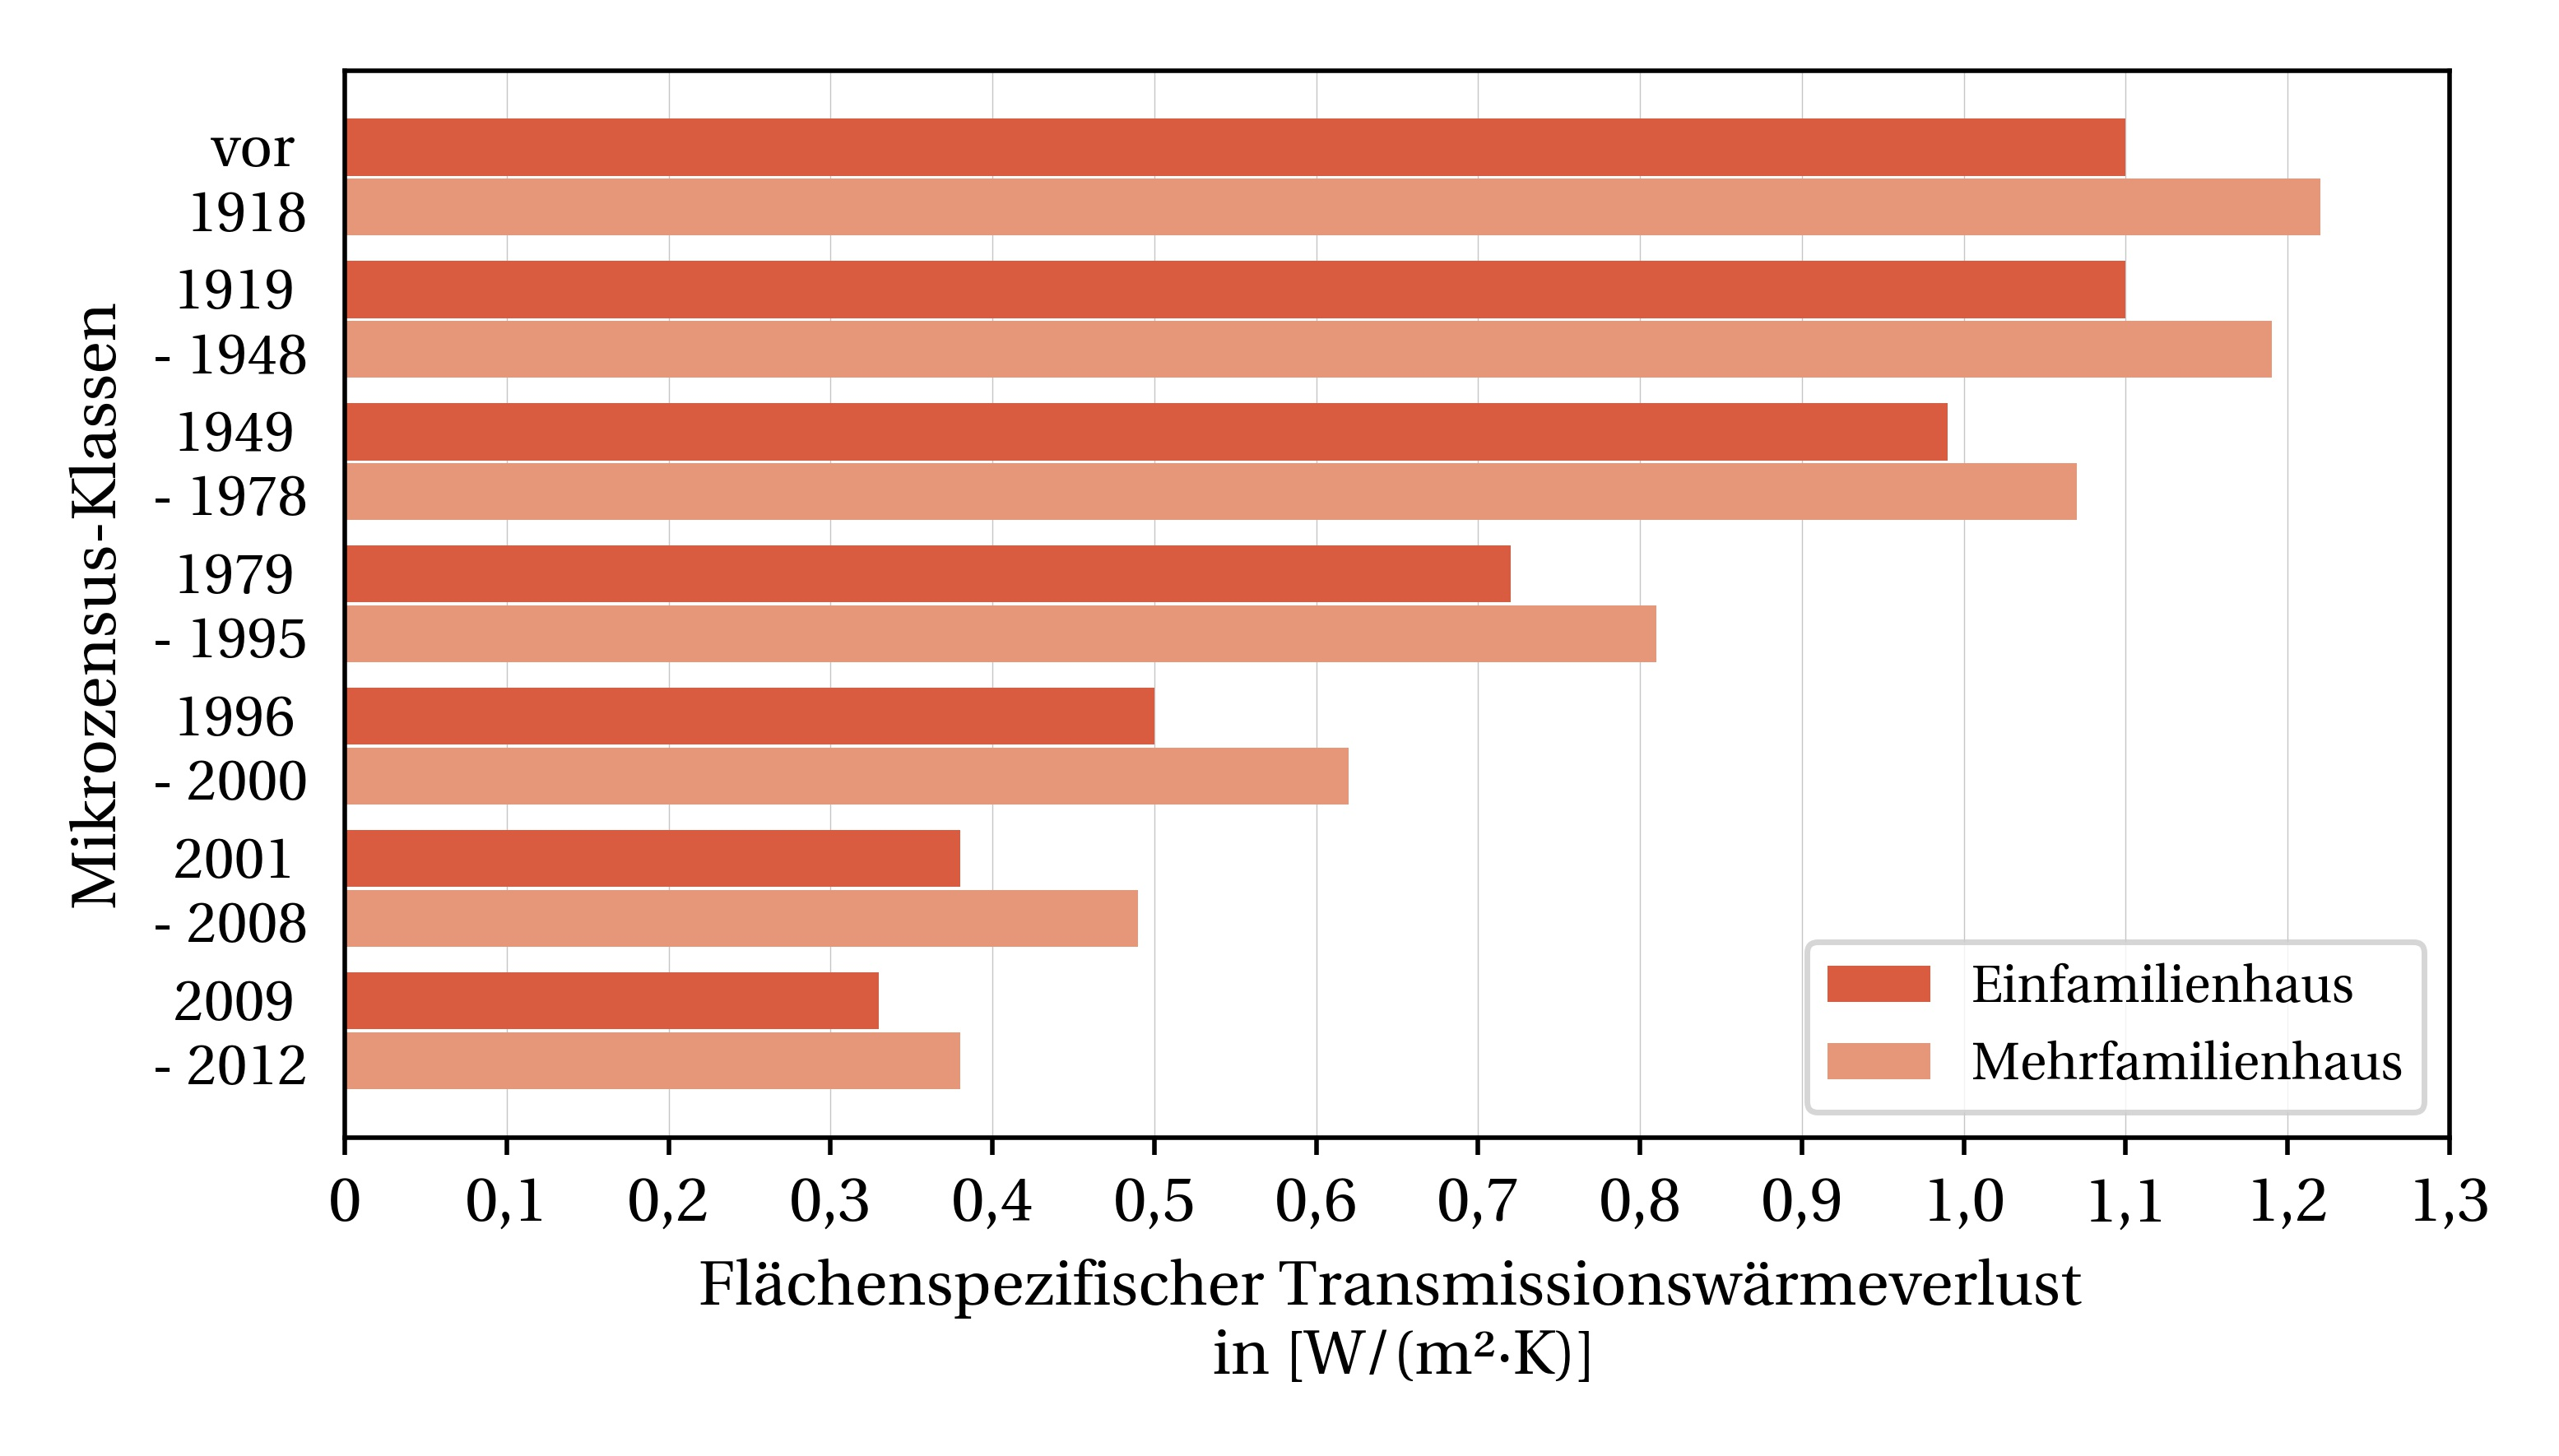
\includegraphics{Pictures/TransmissionswaermekoeffizientBaujahr.jpg}
	\caption{tba}
	\label{fig: Abbildung221} 
\end{figure}

Zu Tabelle \ref{tab: TabelleA1} ist anzumerken, dass sie sich auf den Zustand der Bauteile im damaligen Neubau bezieht. 
Einzige Ausnahme hierbei bilden die Fenster der Zeiträume bis 1978. 
Für diese charakterisierte die Einscheiben-Verglasung den
%Hier doof
%Zeitstrahl mit Transmissionswärmeverlusten
%Auf Grafik Bezug nehmen





\section{Sanierungsstand des deutschen Wohngebäudebestandes}
\label{sec:Sektion 23}

In dem vorangegangen Abschnitt wurde die Entwicklung des Dämmstandard vorgestellt. 
Hierbei wurde sich ausschließlich auf den Neubauzustand bei Fertigstellung des Gebäudes bezogen.
Dieses Kapitel soll nun die Veränderung des Gebäudebestandes aus energetischer Sicht durch Sanierung veranschaulichen.

Abbildung \ref{fig: Abbildung231} zeigt den Anteil der durch nachträgliche Wärmedämmung sanierten Bauteilfläche nach Bauteilen und Gebäudeart.
Zu erkennen ist der große Anteil an sanierter Dachfläche beziehungsweise obere Geschossdeckenfläche.
Dieser liegt für SFH und MFH annähernd gleich bei etwa 57\,\%.
Folglich wurde mehr als die Hälfte der Dachflächen im Altbau nachträglich gedämmt.
Einen leichten Unterschied zwischen den Gebäudearten ist bei den nachträglich sanierten Außenwänden zu beobachten. 
Bei diesem Bauteil wurden bei MFH etwas mehr als 31\,\% mit einer besseren Dämmung versehen, wohingegen es bei den SFH nur etwa ein Viertel waren.
Deutlich weniger Relevanz bei der nachträglichen Dämmung erhielt die Isolierung des Fußbodens beziehungsweise der Kellerdecke. 
Für diese Bauteile wurden bei beiden Gebäudearten nur circa 10\,\% mit einem besseren Wärmeschutz versehen. 

\begin{figure}[H]
	\centering
		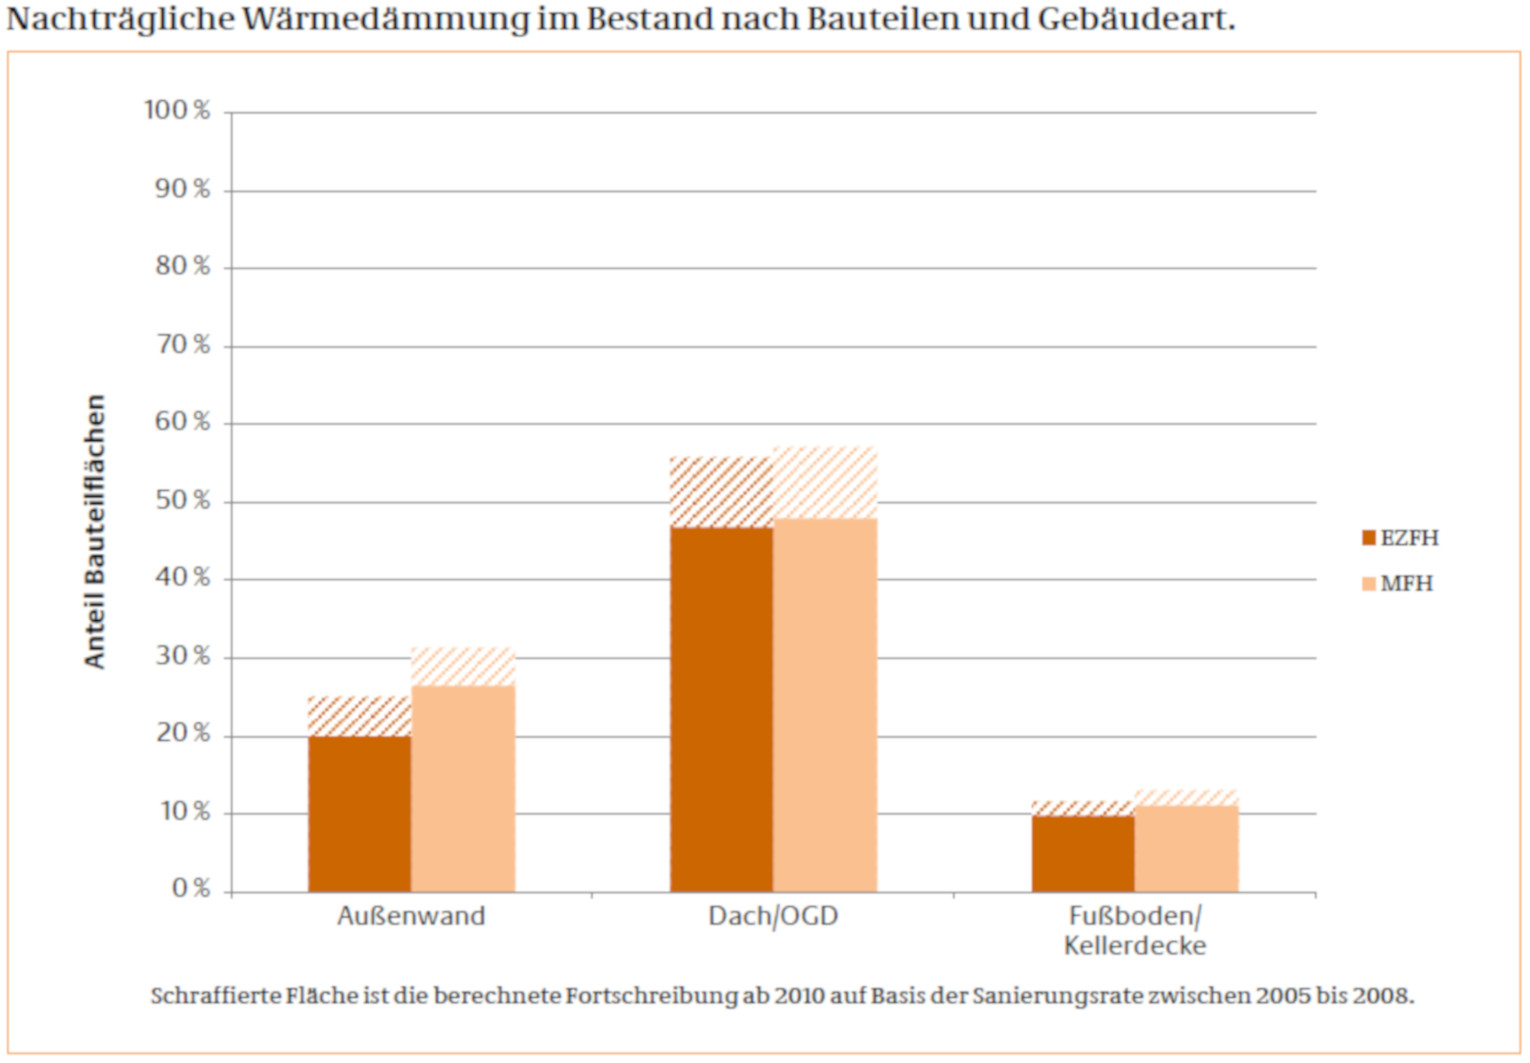
\includegraphics{Pictures/NachtraeglicheSanierung.jpg}
	\caption{\cite{Bigalke.2016}}
	\label{fig: Abbildung231} 
\end{figure}

In Abbildung \ref{fig: Abbildung231} fehlen die Angaben zum Sanierungsstandes der Fenster.
Hierfür ist die Datenlage der Sanierung schwierig, allerdings bietet \cite{Bigalke.2016} eine Schätzung über den Bestand an Fenstern im Jahre 2015.
Tabelle \ref{tab: TabelleA2} gibt verschiedene Verglasungsarten mit deren \(U_g\)-Werten sowie Anzahl und Anteil am gesamten Fensterbestand in Deutschland wieder.
Wie in Gleichung \ref{eq:Gleichung223} dargelegt, beschreibt der \(U_g\)-Wert den Wärmedurchgang durch die Verglasung ohne Berücksichtigung des Fensterrahmens oder der Wärmebrückenbildung.

Obwohl die Einfachverglasung für einen großen Teil des Altbaues den Neubaustandard darstellte, ist deren Anteil am Fensterbestand mit nur noch 3\,\% sehr gering. 
%Aufgrund dessen enorm hohen Wärmedurchgangskoeffizient in Höhe von 5,8\,\(W/(m^2 \cdot K)\) ist die Rückläufigkeit dieser Fensterart als positiv zu bewerten.
Der heutige Bestand der Fenster wird durch unbeschichtetes Isolierglas sowie dem Zweischeiben-Wärmedämmglas dominiert, welche mit 34\,\% und 47\,\% vertreten sind.
Weiterhin ist zu erkennen, dass das Dreischeiben-Wärmeglas bereits 8\,\% des Fensterbestandes stellt, obwohl dieses erst 10 Jahren vor Erhebung der Daten auf den Markt kam.




%\section{Optimierungsmodell}
%\label{sec:Sektion 24}














%Wie in \cite{.2015} dargelegt, werden die Gebäude mit Baujahr älter als 1919 von der Epoche der Gründerzeit geprägt.
%Diese wird durch einen fortschreitenden Städtebau und den Beginn der Industrialisierung des Bauwesens charakterisiert. 
%Aus wärmetechnischer Sicht lässt sich festhalten, dass es zu dieser Zeit kaum Regulationen bezüglich des Wärmeschutzes gab. 
%Einzig die Dicke der Mauerschicht wurde mit 38\,cm empfohlen, wobei den Dämmstoffen geringe Relevanz zugeordnet wurde. 
%Anstatt durch wärmetechnischen Maßnahmen an der Gebäudehülle Heizkosten zu senken, sparte man beim Bau und durch geringes Heizen. \cite{EickeHenning.2011}

%Zwar kam es in dem Zeitraum von \mbox{1919 - 1948} zur zunehmenden Industrialisierung der Baustoffherstellung, allerdings blieb die zuvor genannte Mentalität des kostengünstigen Bauens anstelle von Maßnahmen zum Wärmeschutz erhalten. 
%Auch nach Einführung der DIN 4110 \glqq Technische Bestimmungen zur Zulassung neuer Bauweisen\grqq\,behielt das Vollziegel-Mauerwerk mit 38\,cm Dicke den Stand als Standard im Hochbau. 
%
%\cite{EickeHenning.2011}

%Wie zuvor bereits kurz erläutert, beschreibt die Epoche von \mbox{1949 - 1957} die Nachkriegszeit mit ihrem schnellen Wiederaufbau. 
%Signifikant für die Nachkriegsbauten, ist die Wiederverwertung von Trümmern. 
%Die im Jahr 1952 eingeführte DIN 4108 verkörperte den ersten Ansatz Wärmeschutz normativ zu regulieren. 
%Trotz deren Name \glqq Wärmeschutz im Hochbau\grqq \,beinhaltete die Norm nur einen Mindestwärmeschutz zur Vermeidung bauphysikalischer Schäden durch Schimmelbildung. 
%Dadurch blieb die Nutzung von Dämmstoffen weiterhin die Ausnahme und es wurde auf das bewährte 38\,cm Mauerwerk zurückgegriffen.
%Des Weiteren gab es bis dahin auch keine Normierung der Fenster, sodass hier ferner die Einfach-Verglasung die Konvention darstellte. \cite{EickeHenning.2011}


\chapter{Stand der Technik}


\section{Arten der Optimierung}
\label{sec:Sektion 31}

Die vorliegende Arbeit zielt auf die Bestimmung von energetischen Sanierungsmaßnahmen ab, welche für den deutschen Wohngebäudebestand möglichst kosteneffizient die C0\(_2\)-Emission reduziert.
Hierbei werden neben verschiedenen Möglichkeiten der Energiebereitstellung auch die energetische Qualität verschiedener Komponenten der Gebäudehülle betrachtet.
Dadurch ergibt sich eine hohe Anzahl an möglichen Kombinationsmöglichkeiten der Maßnahmen und Technologien.
Um aus dieser Komplexität ein Optimum zu bestimmen, ist es sinnvoll, ein rechnergestütztes Optimierungsprogramm als Werkzeug zu nutzen.

Eine Optimierung wird immer durch ein Ziel charakterisiert.
In einem mathematischen Sinne wird dieses als Zielfunktion beschrieben, welches es zu minimieren oder maximieren gilt.
Durch Rahmenbedingungen, auch Nebenbedingungen oder Restriktionen genannt, wird die Menge der zulässigen Lösungen beschränkt.
Dieser Lösungsraum wird durch Gleichungen oder Ungleichungen formuliert.
Sowohl die Zielfunktion als auch die Nebenbedingungen werden durch Variablen abgebildet.
Diese können anschaulich als Stellschrauben beschrieben werden.\cite{Schellong.2016}\\
Zusammenfassend kann eine Optimierung als das Lösen einer Zielfunktion in einem von Restriktionen beschränkten Lösungsraum durch eine Kombination von Variablen umschrieben werden. 

Im Folgenden stellt dieses Kapitel verschiedene Arten der Energiesystemoptimierung sowie diverse Beispiele an Optimierungsprogramme aus der Literatur vor, um letztlich das im Rahmen dieser Arbeit verwendete Programm in \ref{sec:Sektion 32} zu beschreiben.

Zur Einteilung von Optimierungsprogrammen existieren verschiedene Möglichkeiten.
Bei der Betrachtung der zu Grunde liegenden Variablen erhält man eine Unterteilung.
Hierbei werden die Programme in einer mathematischen Anschauung danach unterteilt, aus welchem Raum die Variablen entstammen.
So wird zwischen diskreten und kontinuierlichen Variablen unterschieden. 
Die diskreten entstammen dem Raum der ganzen Zahlen \(\mathbb{Z}\) und umfassen unter anderem Binärvariablen.
Letztere sind die Menge aus [0; 1] und werden im Rahmen der Energiesystemoptimierung oft als Option der Kaufentscheidung von Energiesystemen oder Schaltzustände der Anlagentechnik genutzt. 
Dabei beschreibt 0 einen ausgeschalteten, beziehungsweise nicht gekauften Zustand und 1 den eingeschalteten/gekauften.
Neben den diskreten Variablen werden auch kontinuierliche in Optimierungsprogrammen genutzt. 
Diese sind als reelle Zahlen \(\mathbb{R}\) definiert und beschreiben beispielsweise Kapazitäten, Heizbedarfe oder Wärmeverluste.
Werden in einem Programm diskrete und kontinuierliche Variablen gemischt, so spricht man von einer gemischt-ganzzahligen Optimierung. \cite{Schellong.2016}

Neben den Variablen stellt die Art der Funktionen eine weitere Unterscheidung der Optimierungsprogramme dar.
Bestehen die Restriktionen und die Zielfunktion eines Programmes einzig und allein aus linearen Zusammenhängen, so wird von einem linearen Programm (LP) gesprochen.
Dem gegenüber werden solche Optimierungen, welche auch Nichtlinearitäten abbilden, als nicht-lineare Programme (NLP) bezeichnet.
Oftmals findet man in der Realität nicht-lineare Zusammenhänge, welche mit NLP gut modelliert werden können.
Als ein Beispiel aus der Gebäudeenergiesystemoptimierung sei hier das Teillastverhalten von Wärmeerzeugern genannt.
Jedoch stellt das Lösen von nicht-linearen Gleichungen einen erhöhten Rechenaufwand dar, welcher mit einer deutlich längeren Rechendauer einhergeht.
Somit kann durch die Linearisierung von nicht-linearen Zusammenhängen Rechenzeit zu Kosten von Genauigkeit eingespart werden. 
Die gemischt-ganzzahlige lineare Optimierung wird aufgrund ihrer englischen Bezeichnung (\glqq Mixed Integer Linear Programing\grqq)\,mit MILP abgekürzt, die nicht-lineare analog mit MINLP. \cite{Samsatli.2018} 

In der Literatur werden verschiedene Ansätze und Modelle für die Optimierung von Energiesystemen verfolgt.
Diese werden durch die betrachtete Gebäude- oder Quartiersebene, der Zielfunktion, den zu Grunde liegenden Energiesystemen und der Betrachtung von Auslegungs- oder Betriebsoptimierung des Systems charakterisiert

Iturriaga et al. \cite{Iturriaga.2017} erarbeiten ein allgemeines Modell zur Auslegung von Energiesysteme auf Gebäudeebene. 
Dieses soll alle derzeit verfügbaren Technologien der Wärme-, Kälte- und Elektrizitätsbereitstellung abbilden können.
Hierzu werden die Anlagen unterteilt in solche, welche hohe, mittlere und niedrige Temperaturen erzeugen, Kältemaschinen und elektrische Module.
Thermische und elektrische Energie kann zwischen den jeweiligen Energiebereitstellungstechnologien ausgetauscht werden, um letztlich den Wärme-, Kälte- und Elektrizitätsbedarf des Gebäudes zu decken.
Weiterhin berücksichtigt das Modell neben der Energieerzeugung auch Speicher und Interaktionen mit anderen Gebäuden durch Nah-, Fernwärme- sowie Stromnetze.
Das Modell wird anhand eines Beispielgebäudes im nordspanischen Bilbao getestet.
Hierbei werden 13 verschiedenen Technologien der Wärme- und Elektrizitätserzeugung in Betracht gezogen.
Diese umfassen neben Organic-Rankine-, Gasturbinen- und Verbrennungsmotoren-Blockheizkraftwerke (BHKW) auch verschiedene solarthermische Anlagen (CPC, Vakuumröhrenkollektoren, Flachkollektoren), Biomasse-, Gas- und Brennwertkessel, Luft-Wasser-Wärmepumpen (WP) und diverse Photovoltaik-Anlagen (PV) (amorphe, mono- und polykristalline Solarmodule).
Die stückweise Linearisierung des nicht-linearen Teillastverhaltens der Anlagen führt zu rein linearen Gleichungen und somit zu einem MILP Problem.
Als Zielfunktion ist die Minimierung der annualisierten Kosten definiert. 
Diese setzen sich aus Investitionen, jährlichen variablen Kosten, Energiebezugskosten sowie Gewinnen aus dem Verkauf an überschüssiger Wärme, Kälte oder Elektrizität zusammen.
Als Restriktionen der Optimierung sind technologische Nebenbedingungen der Anlagentechnik, die Bedarfserfüllung des Gebäudes, gebäudespezifische Rahmenbedingungen sowie die möglichen Ausprägungen der Variablen aufgeführt.

In \cite{Pinzon.23.04.201726.04.2017} wird ein Modell von Pinzon et al. zur Optimierung der jährlichen Elektrizitätskosten unter Berücksichtigung der Behaglichkeit der Bewohner vorgestellt.
Die Berechnung dieser Kosten berücksichtigt den Strombedarf zu Heiz- oder Kühlzwecken, zur Beleuchtung sowie Ersparnisse aus PV.
Weiter existiert die Option erzeugten Strom, Wärme oder Kälte in einem Energiespeicher (ES) zu lagern.
Wie in Iturriaga et al. \cite{Iturriaga.2017} werden nicht-lineare Gleichungen durch stückweise Linearisierung in lineare gewandelt.
Dadurch handelt es sich bei dem Programm von Pinzon et al. um ein betriebsoptimierendes MILP Problem.
Als Zielfunktion ist die Minimierung des Strombedarfes und somit der Stromkosten beschrieben.
Der Bedarf setzt sich aus dem Verbrauch der zuvor genannten Komponenten zusammen.
Als Nebenbedingungen werden die Nutzung der PV-Anlagen, des ES, des Klimageräts und der Beleuchtung sowie die Einhaltung des thermischen Komforts definiert.
Bei letzterem werden auch die Wärmeträgheit des Luftvolumens im Raum, sowie der Wärmeverlust durch den Infiltrationsluftvolumenstrom, also durch Undichtheiten in der Gebäudehülle, berücksichtigt.

In Risbeck et al. \cite{Risbeck.2017} wird der optimale Betrieb von Lüftungssystemen zum Kühlen und Wärmen in kommerziellen Gebäuden, also Nichtwohngebäuden, untersucht.
Hierzu werden diskrete Variablen zum Modellieren des An- und Abschaltens der Komponenten sowie kontinuierliche zur Abbildung der Lasten und Speicherstände genutzt.
Als Zielfunktion werden minimale Betriebskosten bei Einhaltung des thermischen Komforts im Gebäude formuliert.
Auch Risbeck et al. wandeln nicht-lineare Geräteverhalten durch stückweise Linearisierung in lineare um und modellieren somit ein MILP.
Dadurch wird die Rechenzeit verkürzt und das Programm kann in Echtzeit auf Preisänderungen, Bedarfsschwankungen und Wetteränderungen eingehen.
Als Nebenbedingungen der Optimierungsaufgabe werden neben der Temperierung verschiedener Gebäudezonen auch die optimale Nutzung der zur Verfügung stehenden Speicher beachtet.

Zhu et al. stellen in \cite{Zhu.2019} eine multikriterielle Energsystemoptimierung vor.
Hierbei werden thermische und elektrische Speicher zur optimalen Kapazitätsauslegung untersucht und als übergeordnetes Modell definiert.
Weiter wird hierfür der Betrieb der Energieerzeuger optimiert, was das untergeordnete Modell umschreibt.
Zur Deckung des Wärme- und Elektrizitätsbedarfs werden eine Sole-WP, PV und Strombezug aus dem Netz modelliert.
Die Energiespeicherung erfolgt durch einen sensiblen Wasserspeicher und eine Batterie.
Ein Teil der nicht-linearen Gleichungen werden linearisiert. 
Da jedoch weiterhin nicht-lineare Zusammenhänge in dem Programm existieren, handelt es sich bei dem Modell um ein MINLP, welches Energiesysteme auf Gebäudeebene optimiert.
Als Zielfunktion des übergeordneten Modells wird die Minimierung der jährlichen Gesamtkosten festgelegt.
Das untergeordnete Optimierungsmodell minimiert die jährlichen Betriebskosten der Energieerzeuger.

Eine glechzeitige Betrachtung von Anlagentechnik und Gebäudehülle ist in Asadi et al. zu finden \cite{Asadi.2012}.
Hierbei handelt es sich zum einen um ein MINLP und zum anderen um eine multikriterielle Optimierung, bei welcher dem Programm mehrere Zielfunktionen übergeben werden.
Das Modell betrachtet neben Dämmarten und -stärke der Außenwand und des Dachs auch den Fenstertyp sowie Solarkollektoren. 
Hierzu wird für jedes Bauteil zwischen unterschiedlichen Sanierungsszenarien unterschieden.
Weiter wird der Energiebedarf des Gebäudes vereinfacht als Summe des Wärme-, Kälte- und Warmwasserbedarfes berechnet.
Ziel des Programmes ist die Bestimmung des kosten- und emissionsoptimalen Energiesystems.

In \cite{Wouters.2014} modellieren Wouters et al. Haushalte, die auf Quartiersebene thermische und elektrische Energie untereinander austauschen können.
An Anlagentechnik stehen Brennwertkessel, BHKWs, ES, PV-Anlagen und kleine Windkraftanlagen (WKA) zur Verfügung.
Als Zielfunktion ist die Minimierung der Annuität durch optimale Anlagenwahl, -auslegung und -betrieb definiert.
Das Programm wird nur mit linearen Gleichungen modelliert, sodass es sich um ein MILP handelt.
Weiter werden Einflüsse regulatorischer Maßnahmen untersucht und darauf aufbauend zwei Standorte mit ähnlichen klimatischen Bedingungen in Griechenland und Australien miteinander verglichen.

Das Optimierungsmodell von Harb et al. \cite{Harb.2016} bestimmt die optimale Anlagenauswahl zur Wärmeerzeugung von Einzelwohngebäuden oder Quartieren.
Es werden Mikro-BHKWs, Wärmepumpen, Elektroheizstäbe, PV, thermische Speicher, Kessel sowie Nahwärmenetze in Betracht gezogen.
Das MILP von Harb et al. benennt als Ziel die Minimierung der jährlichen Kosten, welche sich aus annualisierten Investitionen, Bedarfskosten sowie den variablen Kosten zusammensetzen.
Das Modell von Harb et al. zeichnet aus, dass die Einspeisevergütung von PV-Strom sowie die Förderung von BHKW produzierter Elektrizität in die wirtschaftliche Betrachtung mit einfließen.

Eine simultane Betrachtung der Energieerzeuger und der Gebäudehülle liegt in Schütz et al. \cite{Schutz.2017} vor.
Hier werden sowohl der Betrieb als auch die Auslegung des Gebäudeenergiesystems optimiert.
Das Programm berücksichtigt neben Energieerzeugern und -speichern wie Kessel, BHKW, Elektroheizstäbe (EHS), WP, Solarthermie, PV und ES auch energetische Ertüchtigungen der Außenwand, der Fenster, des Daches und der Bodenplatte.
Als Optimierungsziel kann zwischen Jahres-Kosten- und Emissionsoptimierung gewählt werden.
Weiter besteht die Möglichkeit einer Pareto-Optimierung, bei welcher die nicht gewählte Zielfunktion als Nebenbedingung das Modell beschränkt.

In Tabelle \ref{tab: Tabelle311} sind die zuvor vorgestellten Programme der Energiesystemoptimierung mitsamt ihren charakteristischen Eigenschaften aufgeführt.

\begin{table}[H] \centering
\begin{tabular}{|l|l|l|l|l|}
\hline
\rowcolor[HTML]{C0C0C0} 
Autor & \begin{tabular}[c]{@{}l@{}}Art der\\ Optimierung \end{tabular} & \begin{tabular}[c]{@{}l@{}}Ebene/ \\ Betrachtung \end{tabular} & Energiesysteme & \begin{tabular}[c]{@{}l@{}}Zielfunktion\\ (Minimierung von...)\end{tabular} \\ \hline
Iturriaga et al. & MILP & \begin{tabular}[c]{@{}l@{}}Gebäude\\ Auslegung\end{tabular} & alle & Jährlichen Kosten \\ \hline
\rowcolor[HTML]{EFEFEF} 
Pinzon et al. & MILP & \begin{tabular}[c]{@{}l@{}}Gebäude\\ Betrieb\end{tabular} & PV, ES,Klimageräte & \begin{tabular}[c]{@{}l@{}}Jährlichen Elektri-\\ zitätskosten\end{tabular} \\ \hline
Risbeck et al. & MILP & \begin{tabular}[c]{@{}l@{}}Gebäude\\ Betrieb\end{tabular} & Lüftungssysteme & \begin{tabular}[c]{@{}l@{}}Jährlichen Betriebs-\\ kosten\end{tabular} \\ \hline
\rowcolor[HTML]{EFEFEF} 
Zhu et al. & MINLP & \begin{tabular}[c]{@{}l@{}}Gebäude\\ Auslegung und\\ Betrieb\end{tabular} & PV, WP, ES & \begin{tabular}[c]{@{}l@{}}Jährlichen Betriebs-\\ kosten\end{tabular} \\ \hline
Asadi et al. & MINLP & \begin{tabular}[c]{@{}l@{}}Gebäude\\ Auslegung\end{tabular} & \begin{tabular}[c]{@{}l@{}}Sanierung von Wand, \\ Dach, Fenster/\\ Solarkollektoren\end{tabular} & \begin{tabular}[c]{@{}l@{}}Kosten und\\ Emissionen\end{tabular} \\ \hline
\rowcolor[HTML]{EFEFEF} 
Wouters et al. & MILP & \begin{tabular}[c]{@{}l@{}}Quartier\\ Auslegung und \\ Betrieb\end{tabular} & \begin{tabular}[c]{@{}l@{}}Kessel, BHKW, ES, \\ PV, WKA\end{tabular} & Jährlichen Kosten \\ \hline
Harb et al. & MILP & \begin{tabular}[c]{@{}l@{}}Gebäude/\\ Quartier\\Auslegung\end{tabular} & \begin{tabular}[c]{@{}l@{}}Mikro-BHKW, WP,\\ EHS, PV, \\ thermische ES, Kessel, \\ Nahwärmenetz\end{tabular} & Jährlichen Kosten \\ \hline
\rowcolor[HTML]{EFEFEF} 
Schütz et al. & MILP & \begin{tabular}[c]{@{}l@{}}Gebäude\\ Auslegung und \\ Betrieb\end{tabular} & \begin{tabular}[c]{@{}l@{}}Kessel, BHKW, \\ EHS, WP, Solarthermie, \\ PV, ES/\\ Sanierung von Wand, \\ Dach, Fenster, Boden\end{tabular} & \begin{tabular}[c]{@{}l@{}}Kosten und/\\ oder Emissionen\end{tabular} \\ \hline
\end{tabular}
\caption{Übersicht diverser Ansätze der Energiesystemoptimierung in der Literatur}
\label{tab: Tabelle311}
\end{table}


\section{Referenzmodell als Grundlage dieser Arbeit}
\label{sec:Sektion 32}

Im Rahmen der vorliegenden Arbeit wird ein Programm zur Kosten- oder Emissionsoptimierung von Gebäudeenergiesystemen erweitert.
Neben einer Auswahl an Anlagentechniken zur Energiebereitstellung stehen Maßnahmen zur energetischen Ertüchtigung der Gebäudehülle zur Verfügung. 
Hierbei werden ähnlich wie bei Asadi et al. \cite{Asadi.2012} und Schütz et al. \cite{Schutz.2017} Außenwände, Fenster und Dächer sowie zusätzlich die Grundplatte betrachtet.
Die dem Programm zu Grunde liegende Anlagentechnik ist in Tabelle \ref{tab: Tabelle321} aufgeführt.
Die Entscheidung für verschiedene Anlagen oder Maßnahmen an der Hülle erfolgt durch diskrete Binärvariablen, wohingegen die Auslegung und der Betrieb durch kontinuierliche Variablen modelliert wird.
Wie in Iturriaga et al. \cite{Iturriaga.2017}, Pinzon et al. \cite{Pinzon.23.04.201726.04.2017} und Risbeck et al. \cite{Risbeck.2017} erfolgt eine Linearisierung der nicht-linearen Gleichungen, sodass es sich um ein MILP handelt.
Die Zielfunktion der Optimierung kann entweder zur Minimierung der annualisierten Kosten oder CO\(_2\)-Emissionen gesetzt werden.
Des weiteren besteht die Möglichkeit eine Pareto-Optimierung durchzuführen, bei welcher ein Gebäudeenergiesystem unter Berücksichtigung der Kosten- und Emissionsoptimierung ermittelt wird.

Das zu berechnende Gebäude wird eingangs anhand verschiedener Parameter durch den Nutzer beschrieben.
Hierzu zählen unter anderem das Baujahr, die Gebäudegröße und der Standort.
Anhand dieser Eingabewert greift das Programm auf hinterlegte Daten zu, um weitere Parameter in das Programm mit aufzunehmen.
Weiter werden die 365 Tage eines Jahres in einigen wenigen, repräsentativen Typtagen zusammengefasst, um somit die Komplexität des Problems zu reduzieren.
Bei dem eigentlichen Optimierungsprozess wird ein Gleichungssystem basierend auf den zuvor gewählten und eingelesenen Parametern zur Minimierung der Zielfunktion gelöst.
Nach der Optimierung gibt das Programm Daten zu dem gewählten Energiesystem, den Kosten und den Emission aus, die dann vom Nutzer ausgewertet werden.
In Abbildung \ref{fig: Abbildung321} ist der Programmablauf schematisch skizziert.

\begin{figure}[H]
	\centering
		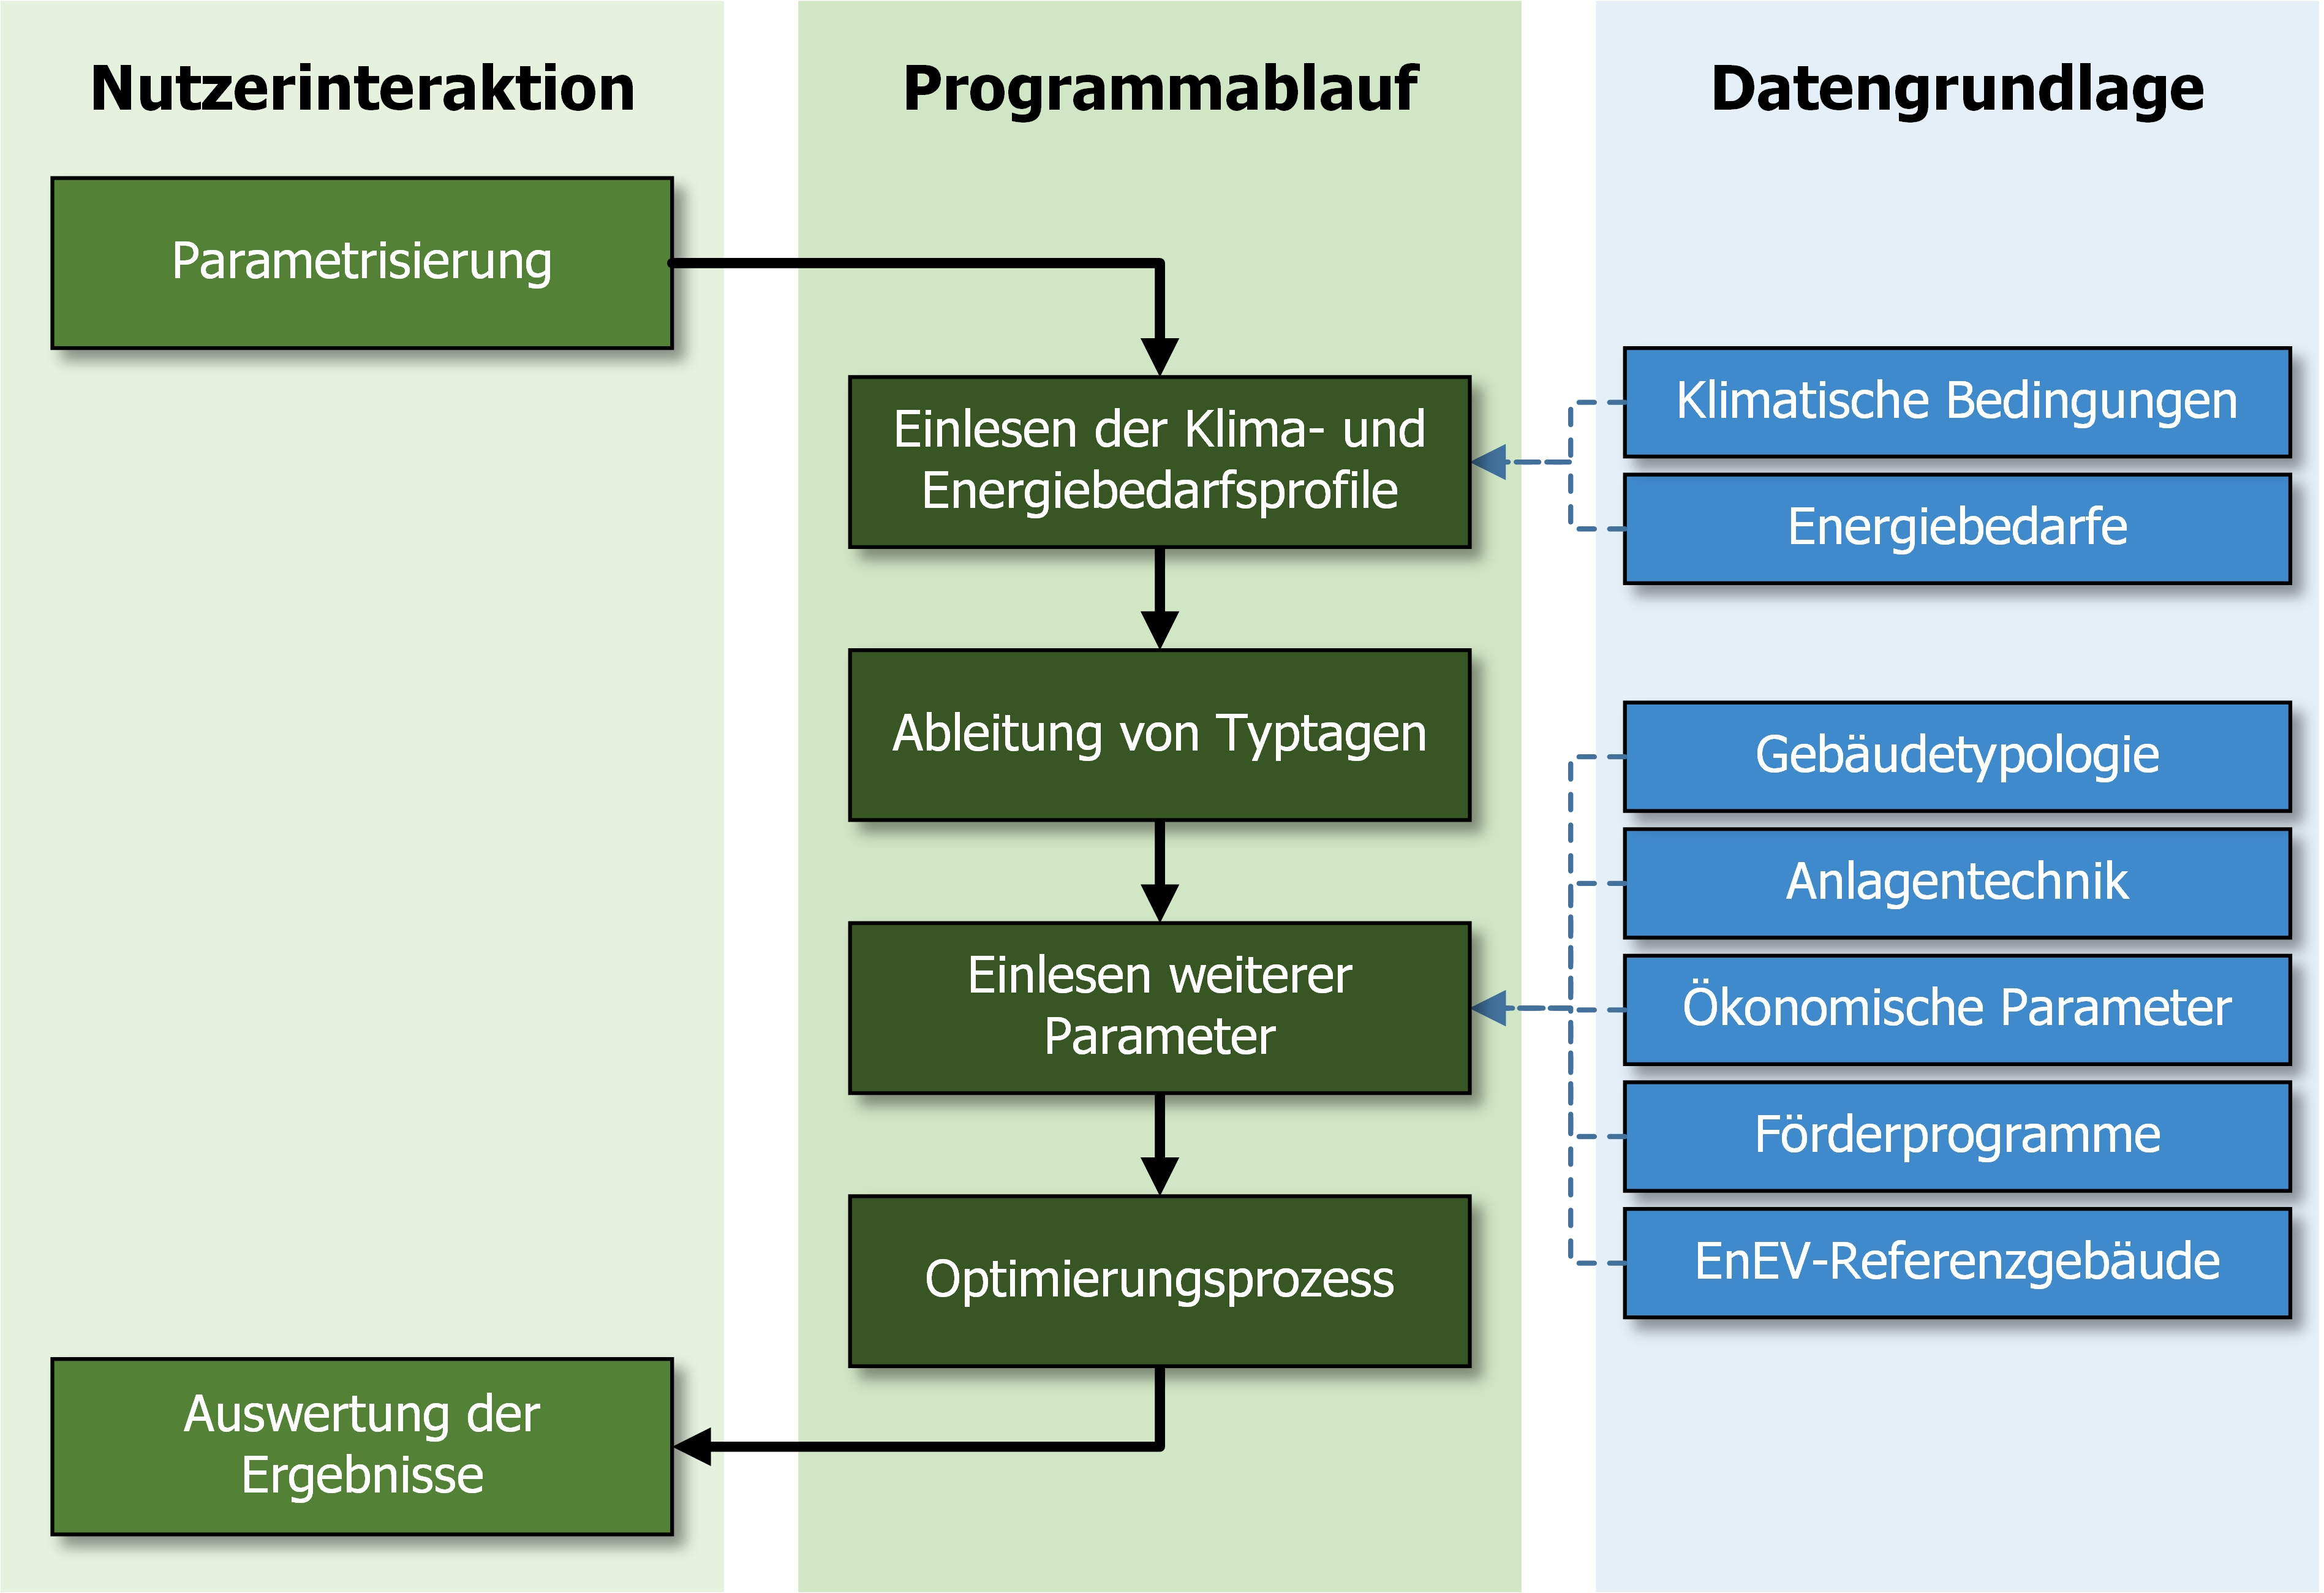
\includegraphics{Pictures/ProzessOptiProgramm.jpg}
	\caption{Schematischer Ablauf des Optimierungsprogrammes}
	\label{fig: Abbildung321} 
\end{figure}

Zunächst erfolgt die Parametrisierung des Gebäudes durch den Nutzer.
Hier werden Gebäudetyp, -alter und -lage sowie Wohnungsanzahl, Wohnfläche je Wohnung, Haushaltsgröße und qualitative Angaben zum Strom- und Trinkwarmwasserbedarfs definiert.
In Bezug auf den Gebäudetyp stehen die TABULA-Klassen Einfamilien-, Reihen-, Mehrfamilienhaus und Apartment-Block zur Wahl.
Auch die Baualtersklassen basieren auf TABULA-Unterteilungen und gliedern sich in 12 Klassen im Zeitraum von 1860 bis 2010.
Bei der Gebäudelage stehen dem Nutzer 15 verschiedene Standorte aus verschiedenen Klimaregionen Deutschlands zur Auswahl.
Eine Übersicht über die möglichen Ausprägungen der Inputparameter Gebäudealter und -lage ist Tabelle \ref{tab: TabelleA3} zu entnehmen. \cite{Loga.102012}

Wie in Abbildung \ref{fig: Abbildung321} dargestellt, startet in einem nächsten Schritt der Programmablauf mit dem Einlesen der Klima- und Energiebedarfsprofile.
Auf Basis der übergebenen Angaben wird auf eine Datengrundlage zurückgegriffen.
So werden anhand des Gebäudestandortes entsprechend jährliche Klimaprofile genutzt.
Diese entsprechen dem Testreferenzjahr des Deutschen Wetterdienstes, welches für den Betrachtungszeitraum von 1981 bis 2010 einen repräsentativen Witterungsverlauf beschreibt \cite{try}.
Neben einem Umgebungstemperaturverlauf liefern die Profile solare Einstrahlungen und sind stündlich, also in 8760 Zeitpunkte, aufgeteilt.
Weiter werden Strom- und Trinkwarmwasserbedarfsprofile sowie Profile der internen Gewinne eingelesen.
Im Falle der Einfamilien- und Reihenhäuser hängen diese von der Haushaltsgröße ab und bei den Mehrfamilienhäusern sowie Apartment-Blocks von der Wohnungsanzahl.
Außerdem bedingen die Angaben zur Höhe des Strom- und Trinkwarmwasserbedarfes die Auswahl der Profile.
Die eingelesenen Verläufe basieren auf stochastischen erzeugten Profilen des deutschen Stromspiegels und bilden Grundlasten sowie Lastspitzen ab \cite{stromspiegel}.
Wie bei den Klimaprofilen sind auch diese als stündliche Werte über ein Jahr aufgetragen.

Da eine Optimierung über jede Stunde eines Jahres mit einem großen Rechenaufwand einhergeht, erfolgt anhand der eingelesenen Profile eine Ableitung von Typtagen.
An Tagen mit vergleichbaren Witterungsverläufen ähneln sich die Energiebedarfsprofile, sodass diese im Rahmen des Programmes mit Hilfe eines Clusteringvorgangs zusammengefasst werden \cite{Dubielzig.2007}.
Um einerseits saisonale Effekte abzubilden und aussagekräftige Ergebnisse zu erhalten und andererseits die Rechenzeit des Programmes zu verkürzen, werden die 8760 Stunden eines Jahres in 8 Typtagen mit 192 Zeitpunkten zusammengefasst.
Diese besitzen wiederum Gewichtungen, welche in Summe 365 Tage und somit ein Jahr ergeben.

Neben den bereits erläuterten Klima- und Energiebedarfsprofilen wird als nächster Vorgang des Programmablaufes weitere Parameter eingelesen.
So werden für die Bauteile der Gebäudehülle U-Werte für drei Sanierungsszenarien in das Modell mit aufgenommen.
Bei diesen handelt es sich um den Standard-Zustand des parametrisierten Gebäudes im Bestand (\glqq standard \grqq), einer Aufrüstung auf den Standard nach EnEV 2014 (\glqq retrofit\grqq) und einer energetischen Nachrüstung nach heutigem Passivhaus-Standard (\glqq advanced retrofit \grqq) \cite{.2015}.
Zudem werden Faktoren zur Dimensionierung der Fenster-, Dach-, Boden- und Außenwandfläche eingelesen.\\
Schließlich werden auch ökonomische Faktoren zur Bestimmung des Preises einer Sanierungsmaßnahme in das Programm mit aufgenommen. 
Hierbei werden die Investitionen der Gebäudehüllenbestandteile als lineare Funktion ausgedrückt.
Außer bei den Fenstern berechnen sich diese Kosten anhand der zusätzlichen Dämmdicke im Zuge des Sanierungsszenario.
Im Falle der Verglasung wird die lineare Funktion anstelle der Dämmstärke in Abhängigkeit der Verbesserung des U-Wertes aufgestellt.
Die Werte für den y-Achsenabschnitt und die Steigung der linearen Funktionen für die einzelnen Bauteile basieren auf Berechnungen des IWU \cite{Hinz.10.08.2015} und sind in Tabelle \ref{tab: TabelleA4} aufgeführt.
Zusätzlich sind in dieser Tabelle Angaben zu der Nutzungsdauer der Komponenten zu finden, welche aus derselben Quelle entstammen.
Diese werden für die Berechnung der annualisierten Kosten benötigt.\\
Mit den bisher beschriebenen Daten lassen sich die Bedarfe des Gebäudes bestimmen.
Zur Deckung dieser werden verschiedene Energieerzeuger und -speicher zu dem Modell hinzugefügt.
Die Dimensionierung der jeweiligen Technologien erfolgt kontinuierlich.
Um die Investition der Anlagen zu berechnen, existieren Installationskosten mit einer Unterscheidung zwischen Einfamilien- oder Mehrfamilienhaus.
Zudem werden die Steigung und der y-Achsenabschnitt einer linearen Funktion zur Preiskalkulation an das Programm übergeben oder anhand von empirischen Herstellerangaben generiert.
Tabelle \ref{tab: Tabelle321} führt die verschiedenen Technologien, welche im Modell Beachtung finden, auf.

Weiter werden betriebswirtschaftliche Parameter eingelesen.
Hierbei werden neben allgemeinen Faktoren wie dem Betrachtungszeitraum, der Mehrwertsteuer, dem internen Zinssatz und der Inflationsrate auch energieträgerspezifische Kennwerte übergeben.
Bei letzteren handelt es sich zum einen um Preisänderungsfaktoren, welche zukünftige Preisänderungen der Energieträger abbilden und zum anderen um Einspeisevergütung von PV- oder BHKW-Strom und um die Energiesteuer.
In Tabelle \ref{tab: TabelleA6} sind die Parameter mit ihren jeweiligen Werten aufgeführt.\\
Außerdem werden Daten zur Modellierung von Förderprogrammen mitaufgenommen, welche die Verbesserung des Gebäudeenergiesystems subventionieren.
Die Fördergelder beeinflussen die Wirtschaftlichkeit verschiedener Technologien und energetischen Sanierungsmaßnahmen.
Daher werden die leistungsabhängigen Förderhöhen in das Modell mitaufgenommen.
Ferner gibt es für alle Programme Bedingungen, welche für eine Auszahlung erfüllt seien müssen und monetäre Grenzen, in denen sich die Fördersumme minimal und maximal bewegt.
Einen Überblick über die Förderkonditionen und -grenzen werden in Tabelle XXXX dargelegt.\\
Um die Förderungen im Rahmen des KfW-Effizienzhaus-Programms zu erhalten, wird die Sanierungsmaßnahme mit einem EnEV-Referenzgebäude verglichen.
Das Referenzgebäude wird mit derselben Geometrie wie die des parametrisierten Gebäudes ausgeführt.
Allerdings besitzt die Gebäudehülle eine energetische Qualität nach EnEV-Vorgaben.
Die U-Werte der jeweiligen Bauteile nach EnEV sind in Tabelle \ref{tab: Tabelle322} aufgeführt.

\begin{table}[H]\centering
\begin{tabular}{|l|c|}
\hline
\rowcolor[HTML]{C0C0C0} 
Bauteil & U-Werte {[}\(\frac{\text{W}}{m^2 \cdot K}\){]} \\ \hline
Außenwand & 0,28 \\ \hline
\rowcolor[HTML]{EFEFEF} 
Boden & 0,35 \\ \hline
Dach & 0,20 \\ \hline
\rowcolor[HTML]{EFEFEF} 
Fenster & 1,30 \\ \hline
\end{tabular}
\caption{U-Werte der Gebäudehülle für ein EnEV-Referenzgebäude nach EnEV 2009.}
\label{tab: Tabelle322}
\end{table}

Wie aus dem schematischen Ablauf in Abbildung \ref{fig: Abbildung321} zu erkennen ist, folgt nach dem Einlesen aller zuvor erläuterten Parameter der eigentliche Optimierungsprozess.
Als Zielfunktion des Optimierungsprogrammes kann zwischen der Minimierung der annualisierten Kosten oder der CO\(_2\)-Emissionen ausgewählt werden.
Die Kosten setzten sich zusammen aus Investitionen durch die Anschaffung der Anlagentechnik und Ertüchtigung der Gebäudehülle (\(C_{Inv}\)), den Wartungs- und Instandhaltungskosten der Anlagen (\(C_{Var}\)), den Kosten aus dem Bedarf an Elektrizität und Brennstoffen (\(C_{Bedarf}\)), den Fixkosten durch Strom- und Gasbezug (\(C_{Fix}\)) sowie den Gewinnen aus dem Verkauf von Strom (\(R_{Erlös}\)) und die Zuschüsse aus Förderprogrammen (\(R_{Subv}\)).
\begin{equation}
\label{eq:Gleichung321}
C_{total} = \sum C_{Inv} + \sum C_{Var} + \sum C_{Bedarf} + \sum C_{Fix} - \sum R_{Erlös} - \sum R_{Subv}  
\end{equation}
Die Berechnung der Investitionen unterscheidet sich leicht zwischen Energieerzeugern und Hüllensanierung.
Es sei zu erwähnen, dass das Standard-Szenario den Bestandszustand beschreibt und somit nicht mit Kosten verbunden ist.
Letztlich wird in allen Fällen eine totale Investitionssumme berechnet und unter Beachtung der jeweiligen Nutzungsdauer, dem internen Zinssatz und der Inflationsrate annualisiert.
Wie in Tabelle \ref{tab: Tabelle321} zu sehen, unterscheiden sich die Nutzungsdauern der Technologien und der Sanierungsszenarien der Gebäudehülle.
Übersteigt die Nutzungsdauer der Komponente den Betrachtungszeitraum der Kalkulation, wird ein Restwert gebildet und dieser annualisiert.
Im Falle einer geringeren Nutzungsdauer als dem Betrachtungszeitraum berechnet das Programm eine Ersatzinvestition.
Somit ergeben sich auf Basis der unterschiedlichen Nutzungsdauern für keine Technologie oder Sanierungsmaßnahme einen Vorteil gegenüber einer Alternativen.\\
Die betriebsgebundenen Kosten für Wartung und Instandhaltung werden anteilig aus den Investitionen bestimmt und mit einem Faktor zur Inflationsbereinigung multipliziert.\\
Zur Bestimmung der bedarfsspezifischen Kosten wird die Summe aus verschiedenen Energiequellen gebildet. Jeder Summand besteht hierfür aus dem Bedarf des Energieträgers multipliziert mit den leistungsspezifischen Kosten, dem Preisänderungsfaktor der Bezugsgröße und dem Faktor zur Annualisierung der Kosten. 
Eine Ausnahme bilden die BHKWs, da bei diesen der Gaspreis um die Energiesteuer reduziert wird.
Dies ist eine Folge der Förderung durch das KWK-Gesetz.\\
Im Falle der Fixkosten liest das Programm Grundpreise für die Nutzung von Gas und Strom ein.
Für Erdgas betragen diese 138 \(\frac{\text{\euro}}{\text{a}}\) und für den Strombezug 73 \(\frac{\text{\euro}}{\text{a}}\). \\

\begin{table}[H]\centering
\begin{tabular}{|l|c|l|c|}
\hline
\rowcolor[HTML]{C0C0C0} 
\multicolumn{1}{l|}{\cellcolor[HTML]{C0C0C0}\begin{tabular}[c]{@{}l@{}}Technologie\\ Sanierungsmaßnahme\end{tabular}} & \multicolumn{1}{l|}{\cellcolor[HTML]{C0C0C0}\begin{tabular}[c]{@{}l@{}}Nutzungsdauer\\ in Jahren\end{tabular}} & \multicolumn{1}{l|}{\cellcolor[HTML]{C0C0C0}\begin{tabular}[c]{@{}l@{}}Technologie\\ Sanierungsmaßnahme\end{tabular}} & \multicolumn{1}{l|}{\cellcolor[HTML]{C0C0C0}\begin{tabular}[c]{@{}l@{}}Nutzungsdauer\\ in Jahren\end{tabular}} \\ \hline
\rowcolor[HTML]{EFEFEF} 
Brennwertkessel & 20 & Solarthermie & 20 \\ \hline
Luft-Wärmepumpe & 18 & PV & 20 \\ \hline
\rowcolor[HTML]{EFEFEF} 
Sole-Wärmepumpe & 20 & Thermischer Speicher & 20 \\ \hline
Pelletkessel & 20 & Batteriespeicher & 15 \\ \hline
\rowcolor[HTML]{EFEFEF} 
BHKW & 15 & Elektroheizstab & 20 \\ 
\hline \hline
Außenwand & 50 & Dach & 50 \\ \hline
\rowcolor[HTML]{EFEFEF}
Fenster & 50 & Bodenplatte & 50\\ \hline
\end{tabular}
\caption{Anlagentechnik und Maßnahmen der energetischen Ertüchtigung der Gebäudehülle sowie deren Nutzungsdauer im Optimierungsmodell}
\label{tab: Tabelle321}
\end{table}

Die Emission kann als Summe der CO\(_2\)-Freisetzung beschrieben werden, die durch den Bedarf an Brennstoffen entstehen.
Somit setzt sich die Berechnung der Emission aus der Verbrennung von Holz-Pellets (\(E_{Pellet}\)), Gas (\(E_{Gas}\)) und dem Emissionswert des Stromes aus Netzbezug (\(E_{Netz}\)) zusammen.
\begin{equation}
\label{eq:Gleichung322}
E_{total} = E_{Pellet} + E_{Gas} + E_{Netz}
\end{equation}
Die jeweiligen Summanden ergeben sich als Produkt aus dem Bedarf der Bezugsgröße und der leistungsspezifischen Emission der Emissionsquelle.
In Tabelle \ref{tab: Tabelle321} sind die Werte für die Energiequellen Holz-Pellets, Gas und Strom aufgeführt.

\begin{table}[H]\centering
\begin{tabular}{|l|c|}
\hline
\rowcolor[HTML]{C0C0C0} 
Energiequelle & \begin{tabular}[c]{@{}c@{}}CO\(_2\)-Emission\\ in {[}\(\frac{kg_{CO_2}}{kWh}\){]}\end{tabular} \\ \hline
\rowcolor[HTML]{EFEFEF} 
Holz-Pellets & 0,025 \\ 
\hline
Gas & 0,25 \\ 
\hline
\rowcolor[HTML]{EFEFEF} 
Strom & 0,566 \\ 
\hline
\end{tabular}
\caption{Leistungsspezifische Emission der Energieträger \cite{InstitutfurTechnischeGebaudeausrustungDresden.2017}}
\label{tab: Tabelle321}
\end{table}

Die Kombinationsmöglichkeiten zur Erfüllung der Zielfunktionen wird durch den Lösungsraum beschränkt, welcher durch Restriktionen definiert wird.
So wird beispielsweise die Anzahl der PV-Module durch die zur Verfügung stehende Dachfläche limitiert.
Eine zentrale Nebenbedingung stellt die Berechnung des Jahres-Heizenergiebedarf dar.
Diese beschreibt die Wärmemenge, welche durch die Anlagentechnik bereitgestellt werden muss, um das Gebäude auf die Innentemperatur in Höhe von 20\,°C zu heizen.
Zur Berechnung des Jahres-Heizwärmebedarfs wird die DIN V 4701-10 \cite{DeutschesInstitutfurNormunge.V..082003} genutzt.
Wie in Abbildung \ref{fig: Abbildung321} zu erkennen ist, setzt sich der Heizwärmebedarf zusammen aus den Transmissionwärmeverlusten (Q\(_T\)), den Lüftungswärmeverlusten (Q\(_V\)), den solaren Gewinnen (Q\(_S\)) und den internen Gewinnen (Q\(_i\)).
Somit wird der Heizwärmebedarf berechnet als
\begin{equation}
\label{eq:Gleichung3292}
Q_h = Q_T + Q_V - Q_S - Q_i
\end{equation}

\begin{figure}[H] \centering
	\centering
		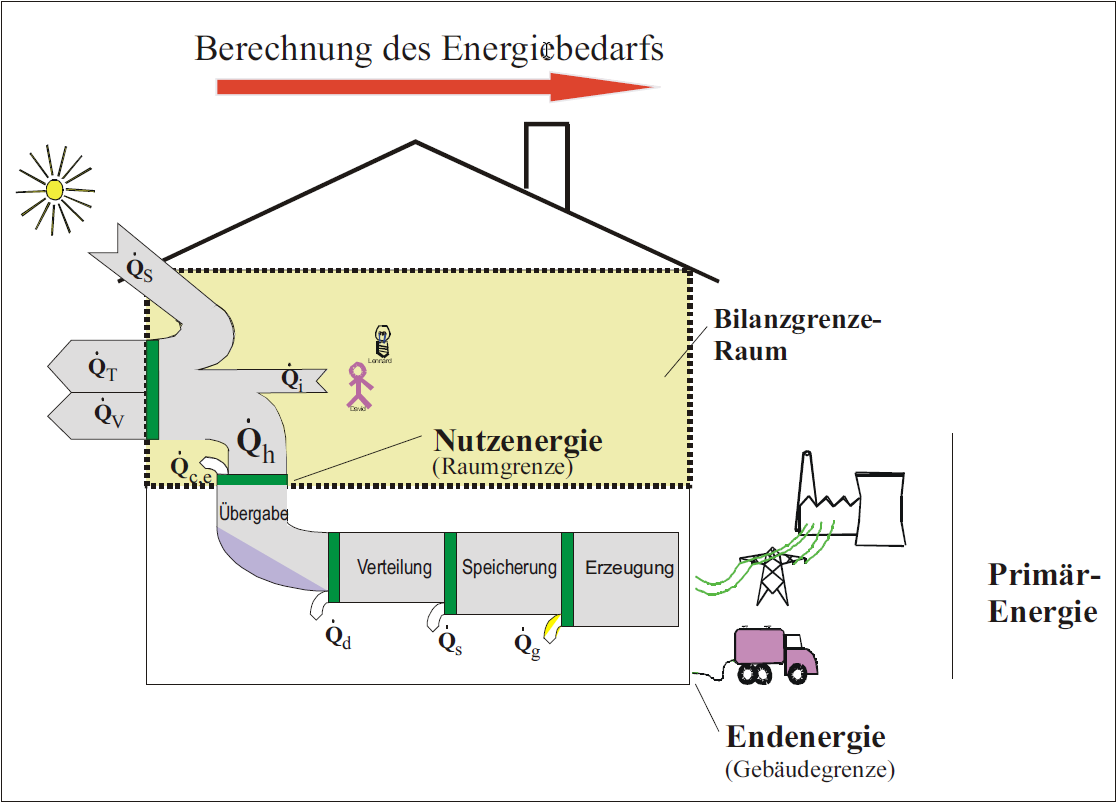
\includegraphics{Pictures/DIN_V_4701_10.png}
	\caption{Schematische Darstellung der Berechnung des Energiebedarfs nach DIN V 4701-10 \cite{DeutschesInstitutfurNormunge.V..082003}}
	\label{fig: Abbildung321} 
\end{figure}

Die Ermittlung der Transmissionswärmeverluste erfolgt anhand des Monatsbilanzverfahrens der DIN V 4108-6.
Hier wird der spezifische Transmissionwärmeverlust (H\(_T\)) anhand von Gleichung \ref{eq:Gleichung3293} berechnet.
\begin{equation}
\label{eq:Gleichung3293}
H_T = \sum U_i \cdot A_i + H_u + L_S + H_{WB} + \Delta H_{T,FH}
\end{equation}
Hierbei wird die Fläche (A) eines Bauteils i mit dessen U-Wert multipliziert, um den Wärmeverlust aufgrund des Wärmedurchgangs durch das Bauteil zu bestimmen.
Weiter wird der Einfluss durch Wärmebrücken mittels H\(_{WB}\) und der Wärmeverlust bei anderer Temperaturdifferenz anstatt Innen- und Außentemperatur durch den thermischen Leitwert L\(_S\) berücksichtigt.
Da in dem Optimierungsmodell keine Unterteilung in Räume geschieht und von einer durchweg konstanten Innentemperatur ausgegangen wird, entfällt der spezifische Transmissionswärmeverlust durch unbeheizte Räume (H\(_u\)).
Ebenso wird der spezifische Wärmeverlust durch Bauteile mit Flächenheizung (\(\Delta\)H\(_{T,FH}\)) nicht betrachtet.
Nach DIN V 4108-6 werden L\(_S\) und H\(_{WB}\) mit
\begin{equation}
\label{eq:Gleichung3294}
L_{S,i} = F_i \cdot U_i \cdot A_i
\end{equation}
\begin{equation}
\label{eq:Gleichung3295}
H_{WB} = \Delta U_{WB} \cdot A
\end{equation}
bestimmt. 
Der Temperaturkorrekturfaktor (F\(_i\)) definiert einen abweichenden Temperaturunterschied zwischen Innen- und Außentemperatur des Bauteils i und \(\Delta\) U\(_{WB}\) den Wärmebrückeneinfluss.
Durch Einsetzen von Gleichung \ref{eq:Gleichung3295} und \ref{eq:Gleichung3294} in \ref{eq:Gleichung3293} wird der spezifische Transmissionswärmeverlust mit
\begin{equation}
\label{eq:Gleichung3296}
H_T = \sum_{i} A_i \cdot F_i \cdot (U_i + \Delta U_{WB}) \quad \text{mit i} \in \text{[standard, retrofit, advanced retrofit]}
\end{equation}
berechnet.
Die nummerischen Werte der Faktoren F\(_i\) und \(\Delta\) U\(_{WB}\) werden in Tabelle XXXX wiedergegeben.\\
Die U-Werte der Gebäudehülle hängen von der Wahl des Sanierungsszenarios ab.
Mit x\(_{i,k}\) als binäre Entscheidungsvariable des Bauteils i und Szenarios k wird die spezifischen Transmissionswärmeverluste somit im Optimierungsprogramm als
\begin{equation}
\label{eq:Gleichung3297}
H_T = \sum_{k} \sum_{i}  A_i \cdot F_i \cdot (U_{k,i} + \Delta U_{WB}) \cdot x_{k,i} \quad \text{mit k}  \in \text{[Außenwand, Boden, Fenster, Dach]}
\end{equation}

Weiterhin werden Profile der inneren Gewinne eingelesen und somit Q\(_i\) bestimmt.
Die solaren Gewinne werden anhand der DIN V 4108-6 bestimmt durch
\begin{equation}
\label{eq:Gleichung3298}
Q_s = \sum_j I_{s,j} \sum_{i}^{n} A_{s,ji} \quad \text{.}
\end{equation}
Hierbei wird die effektive Kollektorfläche (A\(_s\)) anhand diverser Abminderungsfaktoren (F\(_s\), F\(_c\), F\(_F\), F\(_W\)) und dem wirksamen Gesamtenergiedurchlassgrad (g) berechnet.
Der Gesamtenergiedurchlassgrad wird als G-Wert bezeichnet und hängt von dem energetischen Standard der Verglasung ab.
Mit den eingelesenen solaren Einstrahlungsprofilen, welche für jede Himmelsrichtung j eingelesen werden und der Binärvariable zur Auswahl eines Sanierungsszenarios i der Fenster (x\(_{Fenster}\)) ergeben sich die solaren Gewinne zu
\begin{equation}
\label{eq:Gleichung3299}
Q_s = F_s \cdot F_c \cdot F_F \cdot F_W \cdot \sum_{i} (x_{Fenster, i} \cdot g_i \cdot \sum_{j} ( A_{Fenster, j} \cdot I_{s,j} ))
\end{equation}

Schließlich wird der Jahres-Heizenergiebedarf auch durch die Lüftungswärmeverluste beeinflusst.
Eine wichtige Kenngröße der Lüftungswärmeverluste stellt die Luftwechselrate (n) dar.
Diese beschreibt, wie oft pro Stunde das Volumen einer Zone durch Frischluft ausgetauscht wird.
Die Luftwechselrate ist definiert als
\begin{equation}
\label{eq:Gleichun330}
n = \frac{\Dot{V}_{Luft}}{V_z} \cdot 3600 \quad,
\end{equation}
wobei \(\Dot{V}_{Luft}\) den eintretenden Luftvolumenstrom und V\(_Z\) das Volumen der Zone beschreibt.\\
Die Lüftungswärmeverluste werden in dem Optimierungsprogramm durch das Heizperiodenverfahren in DIN V 4108-6 \cite{DeutschesInstitutfurNormunge.V..Juni2003} modelliert.
Hierzu wird laut Norm von einer Luftwechselrate für ein nicht-luftdichtheitsgeprüftes Gebäude von n = 0,7\,h\(^{-1}\) ausgegangen. 
Des Weiteren wird das Netto-Volumen (V) in der Norm als 0,76-fachen des Brutto-Volumens (V\(_e\)) bestimmt.
Somit ergibt sich mit der Wärmekapazität der Luft (c\(_{p, Luft}\)) und der Luftdichte (\(\rho_{Luft}\)) die spezifische Lüftungswärmeverluste (H\(_V\)) zu
\begin{equation}
\label{eq:Gleichung328}
H_V = 0,76 \cdot V_e \cdot \rho_{Luft} \cdot c_{p, Luft} \cdot n \quad \text{.}
\end{equation}
Zuletzt wird durch Berücksichtigung des Korrekturfaktor aufgrund von Nachtabschaltung der Heizung (f\(_{NA}\)) und des Gradtagzahlfaktor (G\(_t\)) die jährlichen Lüftungswärmeverluste zu
\begin{equation}
\label{eq:Gleichung329}
Q_{V} = H_V \cdot G_t \cdot f_{NA} \cdot 0,024
\end{equation}
berechnet.
Hierbei ist 0,024 der Umrechenfaktor von Tag zu Stunde und Kilowatt zu Watt.\\
Diese jährliche Energiemenge der Lüftungswärmeverluste wird gleichmäßig auf die 8760 betrachteten Zeitpunkte des Jahres aufgeteilt.
\begin{equation}
\label{eq:Gleichung3291}
Q_l = \frac{Q_{V}}{8760}
\end{equation}
Somit sind diese Verluste in dem Modell für jeden betrachteten Zeitpunkt konstant und werden als statisch angesehen.

\newpage

\section{Lüftungswärmeverluste in Wohngebäuden}
\label{sec:Sektion 33}

Lüftungswärmeverluste entstehen durch den Austausch von warmer Raumluft mit kälterer Außenluft.
Man unterscheidet hierbei zwischen maschineller und natürlicher Lüftung \cite{Maas.2017}.
Bei der natürlichen kann weiterhin zwischen Infiltration und Fensterlüftung unterschieden werden.
Somit sind die Verluste vom Nutzerverhalten, der Dichtheit der Gebäudehülle und dem Lüftungskonzept abhängig.
Je nach Ausprägung dieser Faktoren stellen die Lüftungswärmeverluste zwischen 20 bis 70\,\% der Gesamtwärmeverluste eines Gebäudes. 
Den niedrigen Wert findet man im Altbau. 
Durch die schlechte energetische Qualität der Hülle weicht hier zwar viel Luft durch Fugen und kleine Öffnungen, wodurch der Infiltrationsluftvolumenstrom hoch ist, allerdings dominieren die Transmissionswärmeverluste aufgrund der schlechten Dämmeigenschaften der Hüllenbauteile.
Analog hierzu liegt der relative Anteil der Lüftungs- an den Gesamtwärmeverlusten in solchen Gebäuden höher, welche durch gute Isolationseigenschaften der Gebäudehülle geringe Transmissionswärmeverluste besitzen.
In diesen Fällen steigt der Anteil der Lüftungswärmeverlusten an den Gesamtwärmeverlusten des Gebäudes auf 50 bis 70\,\% \cite{Milles.2011}.
So beispielsweise in Niedrigenergiehäusern oder Altbauten mit energetisch ertüchtigter Gebäudehülle. \cite{BorschLaaks.2011}

\begin{figure}[H]
	\centering
		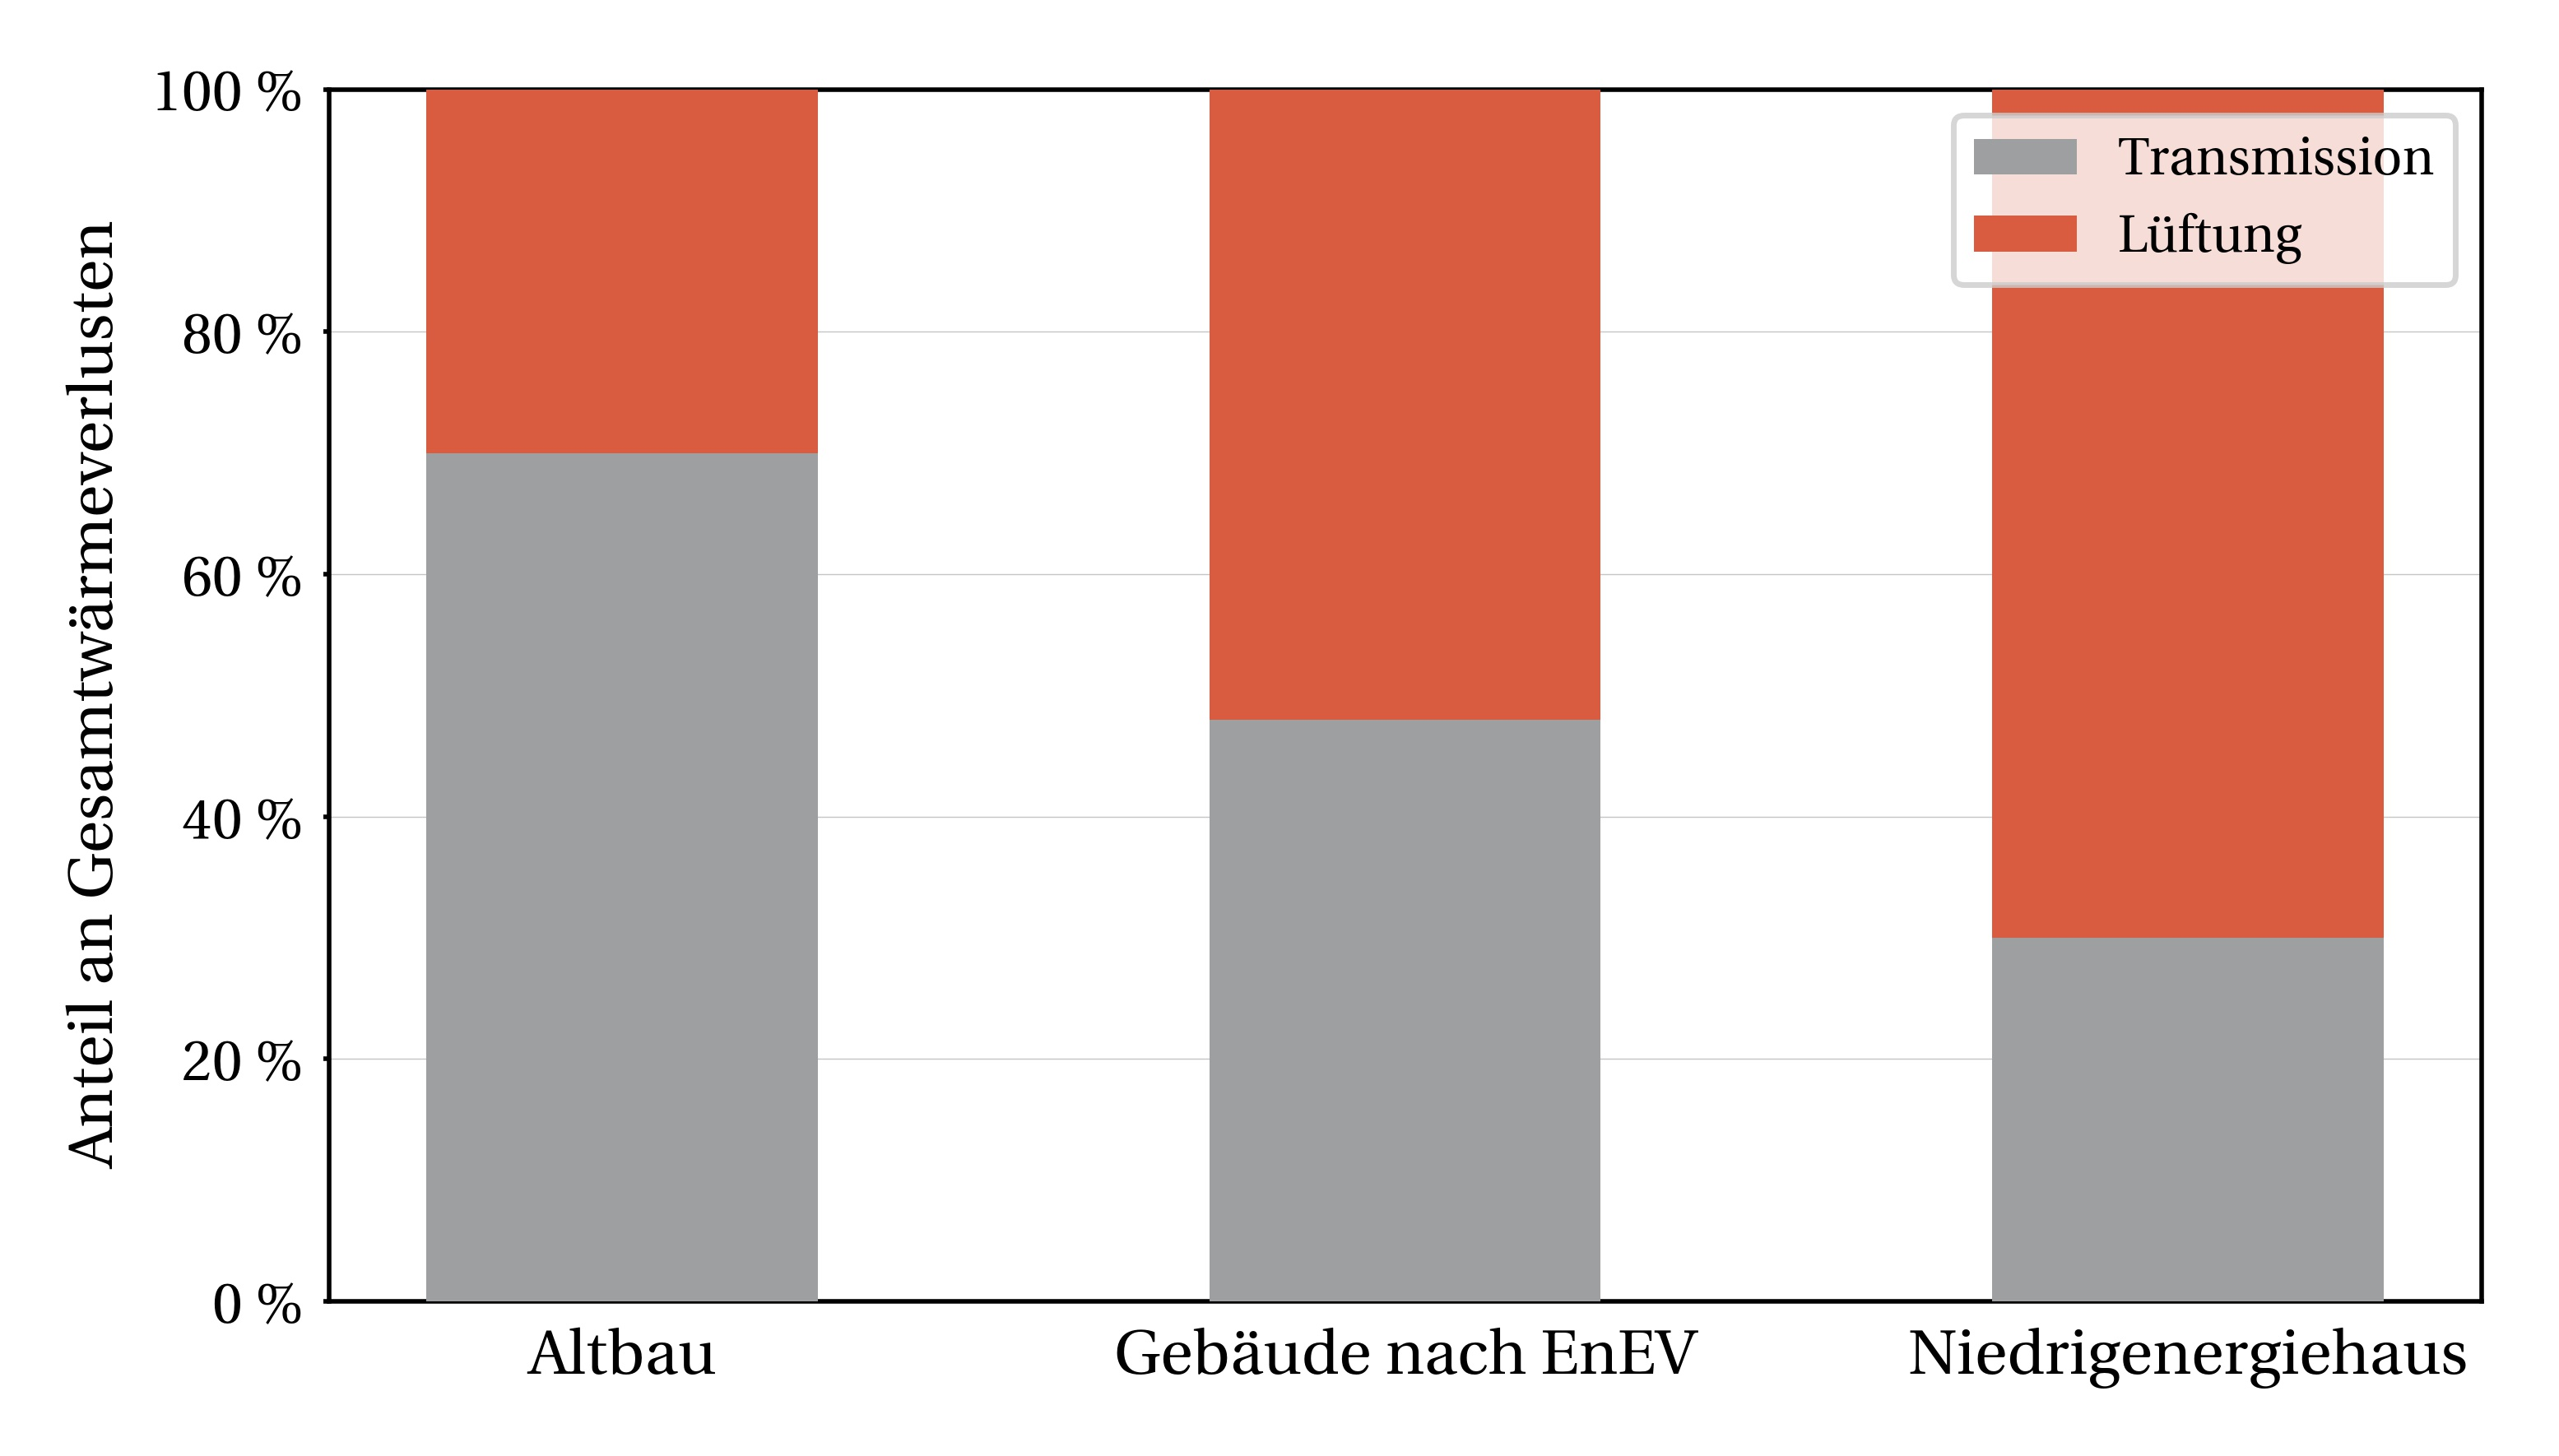
\includegraphics{Pictures/LueftungswaermeverlusteWohngebaeude.jpg}
	\caption{Anteil der Lüftungs- und Transmissionwärmeverluste an den Gesamtwärmeverlusten für unterschiedliche Gebäudestandards \cite{BorschLaaks.2011}}
	\label{fig: Abbildung331} 
\end{figure}


Den Lüftungswärmeverlusten stehen hygienische Aspekte und die Luftqualität gegenüber.
Einerseits muss in einem Gebäude ein Luftaustausch geschehen um Luftfeuchtigkeit und Kohlenstoffdioxid aus den Räumen abzutransportieren.
Andererseits steigen mit zunehmendem Luftaustausch die Wärmeverluste, wodurch ökologisch und ökonomisch nachteilig mehr geheizt werden muss. 

Einen Ansatz zur Bestimmung der Lüftungswärmeverluste bietet die DIN EN 12831 \cite{DINDeutschesInstitutfurNormunge.V..September2017}.
Hier werden diese Verluste des Gebäudes (\(\Phi_{V,build}\)) in z Zonen aufgeteilt.
\begin{equation}
\label{eq:Gleichung331}
\Phi_{V,build} = \sum_{z} \Bigl\langle \Phi_{V,z} \Bigr\rangle
\end{equation}
Die Zonen umfassen jeweils beheizte Räume (i), womit sich die Lüftungswärmeverluste der Zone (z) zu
\begin{equation}
\label{eq:Gleichung332}
\Phi_{V,z} = \rho_{Luft} \cdot c_{p,Luft} \cdot \sum_{i} \Bigl\langle f_{i-z} \cdot q_{v,min,i} \cdot (\theta_{int,i} - \theta_e) \Bigr\rangle
\end{equation}
berechnen lassen.
Hier fließen neben der Luftdichte (\(\rho_{Luft}\)), der spezifischen Wärmekapazität der Luft (c\(_{p,Luft}\)) und der Temperaturdifferenz zwischen Innnen- (\(\theta_{int,i}\)) und Außentemperatur (\(\theta_{e}\)) auch der Mindest-Luftvolumenstrom des Raums i (q\(_{v,min,i}\)) und das Verhältnis zwischen dem Mindestwert des Luftvolumenstroms und des sich ergebenden Luftvolumenstroms (f\(_i-z\)) ein.
Das Produkt aus q\(_{v,min,i}\) und f\(_i-z\) ergibt somit den eintretenden Luftvolumenstrom.
Wird das Gebäude als eine Zone modelliert, erhält man mit q\(_V\) als Produkt von q\(_{v,min,i}\) und f\(_i-z\) 
\begin{equation}
\label{eq:Gleichung333}
\Phi_{V} = \rho_{Luft} \cdot c_{p,Luft} \cdot q_V \cdot (\theta_{int} - \theta_e) \quad \text{.}
\end{equation}
Dies entspricht einer Energiebilanz um die Gebäudehülle, bei welcher der eintretende Volumenstrom dem austretenden entspricht.

Zur Berechnung des eintretenden Luftvolumenstroms q\(_V\) wird dieser in Fensterluftvolumenstrom (q\(_{V, Fenster}\)), Infiltrationsluftvolumenstrom (q\(_{V, Inf}\)) und maschineller Lüftungsvolumenstrom (q\(_{V, Maschinell}\)) aufgeteilt.
Somit ergibt sich q\(_V\) zu
\begin{equation}
\label{eq:Gleichung334}
q_V = q_{V, Fenster} + q_{V, Inf} + q_{V, Maschinell}
\end{equation}
Im Folgenden werden die jeweiligen Komponenten mitsamt ihrer Berechnungsansätzen in der Literatur vorgestellt.

\subsection{Fensterlüftung}
\label{subsec:Sektion 331}

Durch das Öffnen eines Fensters kann ein Bewohner direkt Einfluss auf die Qualität der Raumluft ausüben.
Somit stellt das Nutzerverhalten einen wichtigen Faktor bezüglich der Lüftungswärmeverluste durch die Fenster dar.
Gründe für das Fensteröffnen sind in Fabi et al. \cite{Fabi.2012} wiedergegeben.
Hier erfolgt eine Unterscheidung der ausschlaggebenden Faktoren in die Kategorien \glqq Physische Umweltfaktoren\grqq , \glqq Kontextabhängige Faktoren\grqq , \glqq Psychologische Faktoren\grqq , \glqq Physiologische Faktoren\grqq\, und \glqq Soziale Faktoren\grqq .
Beispiele für die einzelnen Faktoren sind in Tabelle \ref{tab: Tabelle3311} dargelegt.

\begin{table}[H]\centering
\begin{tabular}{|l|l|}
\hline
\rowcolor[HTML]{C0C0C0} 
Einflussfaktoren & Beispiele \\ \hline
 & Temperatur \\ \cline{2-2} 
 & \cellcolor[HTML]{EFEFEF}Luftfeuchte \\ \cline{2-2} 
\multirow{-3}{*}{Physische Umweltfaktoren} & Lärm \\ \hline
\rowcolor[HTML]{EFEFEF} 
\cellcolor[HTML]{EFEFEF} & Dämmstärke der Gebäudehülle \\ \cline{2-2} 
\cellcolor[HTML]{EFEFEF} & Fassadenorientierung \\ \cline{2-2} 
\rowcolor[HTML]{EFEFEF} 
\multirow{-3}{*}{\cellcolor[HTML]{EFEFEF}Kontextabhängige Faktoren} & Heizsystem \\ \hline
 & Thermischer Komfort \\ \cline{2-2} 
 & \cellcolor[HTML]{EFEFEF}Sicherheit \\ \cline{2-2} 
\multirow{-3}{*}{Psychologische Faktoren} & \begin{tabular}[c]{@{}l@{}}Ökologisches und\\ ökonomisches Bewusstsein\end{tabular} \\ \hline
\rowcolor[HTML]{EFEFEF} 
\cellcolor[HTML]{EFEFEF} & Alter \\ \cline{2-2} 
\cellcolor[HTML]{EFEFEF} & Geschlecht \\ \cline{2-2} 
\rowcolor[HTML]{EFEFEF} 
\multirow{-3}{*}{\cellcolor[HTML]{EFEFEF}Physiologische Faktoren} & Gesundheit \\ \hline
 & Interaktionen zwischen Bewohnern \\ \cline{2-2} 
\multirow{-2}{*}{Soziale Faktoren} & \cellcolor[HTML]{EFEFEF}Kollektive Präferenzen \\ \hline
\end{tabular}
\caption{Kategorien der Einflussfaktoren zum Fensteröffnen/-schließen \cite{Fabi.2012}}
\label{tab: Tabelle3311}
\end{table}

Eine weitere Untersuchung des Nutzerverhaltens im Bezug auf das Öffnen und Schließen von Fenstern ist in Calì et al. \cite{Cali.2016b} beschrieben.
Der Unterschied zwischen berechnetem Energiebedarf und gemessenem Energieverbrauch wird unter anderem dem Einfluss der Bewohner auf die Lüftungswärmeverluste zugeschrieben.
Die genannte Diskrepanz zwischen Verbrauch und Bedarf wird als Rebound-Effekt bezeichnet und in \cite{Haas.2000} sowie in \cite{Cali.2016} näher erläutert.
Zur Bewertung von Faktoren, welche das Fensteröffnen oder -schließen durch die Bewohner bestimmen, werden auf umfangreiche Daten eines Forschungsprojekts an drei Mehrfamilienhäusern in Karlsruhe-Rintheim zurückgegriffen.
Eine detaillierte Beschreibung dieser Gebäude und des Daten-Monitorings wird in \cite{Cali.Holistic} vorgestellt.
Auf Basis der erhobenen Werte aus diesem Projekt bestimmen Calì et al. Triebkräfte, welche dazu führen den Fensterzustand zu ändern.
In Tabelle \ref{tab: Tabelle3312} sind die Einflussfaktoren für das Schließen und Öffnen eines Fensters aufgeführt.
Hierbei sind die Gründe nach Wichtigkeit geordnet und beginnen mit dem am häufigst anzutreffenden.

\begin{table}[H]\centering
\begin{tabular}{|l|r|}
\hline
\rowcolor[HTML]{C0C0C0} 
Triebkraft zum Fensteröffnen & Triebkraft zum Fensterschließen \\ \hline
Tageszeit & Außentemperatur \\ \hline
\rowcolor[HTML]{EFEFEF} 
CO\(_2\)-Konzentration im Raum & Tageszeit \\ \hline
Raumtemperatur & CO\(_2\)-Konzentration im Raum\\ \hline
\rowcolor[HTML]{EFEFEF} 
Luftfeuchte im Raum & Raumtemperatur \\ \hline
Außentemperatur & Luftfeuchtigkeit Außen \\ \hline
\end{tabular}
\caption{Triebkräfte zum Öffnen und Schließen eines Fensters \cite{Cali.2016b}}
\label{tab: Tabelle3312}
\end{table}

Aufgrund der zuvor erläuterten Faktoren entscheidet ein Bewohner ein Fenster zu öffnen beziehungsweise zu schließen.
Dadurch lässt sich eine Öffnungsdauer ableiten.
Weiter wird der einströmende Volumenstrom durch den Öffnungswinkel und die Fenstergeometrie beeinflusst.
Aus diesen beiden Faktoren wird die Fensterfläche berechnet, welche effektiv an dem Luftaustausch beteiligt ist.\cite{Hall.2004}

Außerdem zählen neben dem Nutzereinfluss und der Fenstergemoetrie auch die Triebkräfte der Luftbewegung zu wichtigen Faktoren der Fensterlüftung.
Zu diesen gehören zum einen die Temperaturdifferenz zwischen Innen- und Außen und zum anderen die Windgeschwindigkeit \cite{Schild.2013b}.
Durch den Wind entsteht ein Druckgefälle zwischen Innerem des Gebäudes und Umgebung.
Aufgrund des Ausgleichs dieses Gefälles kommt es zum Luftaustausch zwischen dem Gebäude und der Umgebung.
Analog induziert die Temperaturdifferenz eine Luftbewegung zum Ausgleich des thermischen Unterschiedes. \cite{Maas.2017} \\
Oftmals kommt es zu einer Überlagerung dieser beiden Kräfte.
Zudem existiert eine Wechselwirkung zwischen den Triebkräften und dem Nutzerverhalten.
So besteht beispielsweise bei winterlichen Außentemperaturen eine große Temperaturdifferenz, wodurch der eintretende Volumenstrom größer wird.
Gleichzeitig reagiert ein Nutzer mit kurzen Fensteröffnungszeiten aufgrund der thermischen Unbehaglichkeit. 

Zur Bestimmung des Volumenstromes durch ein Fenster existieren verschiedene Ansätze in der Literatur.

\section*{Modell nach Maas}
Auf Basis von experimentellen Untersuchungen unter realen meteorologischen Bedingungen ermittelt Maas \cite{Maas.1995} eine Formel zur Berechnung des Luftvolumenstroms durch ein Fenster.
Hierbei werden neben der Windgeschwindigkeit (u) und der Temperaturdifferenz zwischen Innen und Außen (\(\Delta \theta\)) auch die effektive Fensteröffnungsfläche (A\(_{eff}\)) beachtet. 
Letzteres ist abhängig von der Öffnungsweite des Fensters und bildet Turbulenzeffekte ab.
Somit ergibt sich nach Maas der Volumenstrom zu
\begin{equation}
\label{eq:Gleichung3311}
q_{V, Fenster} = 3600 \cdot \frac{A_{eff}}{2} \cdot \sqrt{(C_1 \cdot u^2 + C_2 \cdot H \cdot \Delta \theta + C_3)} \quad \text{.}
\end{equation}
Hierbei wird A\(_{eff}\) halbiert, da sich bei einem geöffneten Fenster der ein- und ausströmender Volumenstrom die Öffnungsfläche des Fensters teilen.
Der Faktor 3600 wird zum Umrechnen des sekündlichen Volumenstroms in einen stündlichen genutzt.
Die Koeffizienten C\(_1\), C\(_2\) und C\(_3\) werden experimentell bestimmt und stellen Fitkoeffizienten dar.
Ihre nummerischen Ausprägungen sind Tabelle \ref{tab: Tabelle3312} zu entnehmen.

\begin{table}[H] \centering
\begin{tabular}{|l|l|r|l|}
\hline
\rowcolor[HTML]{C0C0C0} 
Größe & Bedeutung & \multicolumn{1}{l|}{\cellcolor[HTML]{C0C0C0}Nummerischer Wert} & Einheit \\ \hline
C\(_1\) & Geschwindigkeitskoeffizient & 0,0056 & --- \\ \hline
\rowcolor[HTML]{EFEFEF} 
C\(_2\) & Temperaturkoeffizient & 0,0037 & \(\frac{m}{s^2 \cdot K}\) \\ \hline
C\(_2\) & Turbulenzkoeffizient & 0,012 & \(\frac{m^2}{s^2}\) \\ \hline
\end{tabular}
\caption{Nummerische Werte der Fitkoeffizienten nach Maas \cite{Maas.1995}}
\label{tab: Tabelle3312}
\end{table}

\section*{Modell nach Hall}
Einen weiteren Ansatz zur Modellierung des Luftvolumenstroms durch ein Fenster liefert Hall \cite{Hall.2004}.
Hierbei werden die Einflüsse des Windes vernachlässigt und nur die Temperaturabhängigkeit des Luftwechsels betrachtet.
Zwar bildet der durch Wind induzierte Luftvolumenstrom durch ein Fenster den größeren Anteil des Gesamtvolumenstroms ab, allerdings wird gezielt ein minimaler Volumenstrom ermittelt, der aus bauphysikalischer und hygienischer Sicht sichergestellt werden muss, um Schäden der Bausubstanz zu vermeiden.
Zudem wird laut Hall ein Fenster bei zunehmendem Wind schnell geschlossen und es kann weiterhin in der Realität zu Windstille kommen, sodass das Modell keinen unwahrscheinlichen Fall abbildet.\\
Weiter werden sich auf Kippfenster bezogen und verschiedene Kippwinkel untersucht.
Die effektive Fensteröffnungsfläche (A\(_{eff}\)) ergibt sich in Abhängigkeit des Öffnungswinkels und der Laibung als die Summe zweier Dreiecke und eines Rechtecks.
Das Rechteck beschreibt hierbei die Fläche oberhalb des geöffneten Fensters und die Dreiecke die Seiten.\\
Ein weiterer Parameter beschreibt die neutrale Höhe (h\(_n\)). 
Diese ist als der Abstand vom Fußpunkt des Fensters zu der Linie, in welcher von einströmender zu ausströmender Luft gewechselt wird, definiert.
Das Verhältnis zwischen h\(_n\) und Fensterhöhe (H) wird mit Z bezeichnet.\\
Außerdem berücksichtigt Hall Reibungsverluste mit dem Koeffizienten C\(_d\), welcher durch Messungen bestimmt wird und die Art der Strömung mit dem Strömungsexponenten (n). 
Letzterer kann Werte zwischen 0,5 und 1 annehmen, wobei 0,5 eine turbulente und 1 eine laminare Strömung beschreibt.
Mit der Erdbeschleunigung (g) ergibt sich der einströmende Luftvolumenstrom zu
\begin{equation}
\label{eq:Gleichung3312}
q_{V, Fenster} = C_d \cdot A_{eff} \cdot \Biggl( 2 \cdot g \cdot H \cdot Z \cdot \frac{\Delta\theta}{\theta_i}\Biggr)^n \quad \text{.}
\end{equation}

\section*{Modell nach DIN EN 12831}
Ein weiterer Berechnungsansatz zur Bestimmung des Luftvolumenstroms durch ein geöffnetes Fenster bietet die DIN EN 12831 \cite{DINDeutschesInstitutfurNormunge.V..September2017}.
Hierbei wird nach ein- oder zweiseitiger Lüftung und der Fassadenausrichtung des Fensters unterschieden.
Bei zweiseitiger Lüftung wird von zwei sich gegenüber befindenden Fenstern ausgegangen.
Unter Vernachlässigung der Fassadenausrichtung ergibt sich der Volumenstrom bei einseitiger Lüftung zu
\begin{equation}
\label{eq:Gleichung3313}
q_{V,open} = \sqrt{q_{V,open,th}^2 + q_{V,open,w}^2}\quad\text{,}
\end{equation}
wobei mit Index \textit{th} der thermisch induzierte und mit Index \textit{w} der durch Wind verursachte Luftvolumenstrom berücksichtigt wird.
Zur Berechnung des thermisch induzierten Anteils wird ein dimensionsloser Durchflusskoeffizient (C\(_D\)) zu 0,61 festgelegt.
Mit diesem lässt sich q\(_{V,open,th}\) durch
\begin{equation}
\label{eq:Gleichung3314}
q_{V,open,th} = \frac{1}{3} \cdot C_D \cdot A_{eff} \cdot \sqrt{\frac{g \cdot h_m \cdot \Delta \theta}{\theta_e}} \cdot 3600 \quad\text{.}
\end{equation}
ausdrücken.
Außer dem Faktor h\(_m\), welcher die mittlere Höhe der Fensteröffnung beschreibt, sind alle anderen Parameter bereits bekannt.
Für die Gleichung des durch Wind verursachten Volumenstroms wird die Windgeschwindigkeit in Fassadenhöhe (v\(_{fac}\)) benötigt.
Mit der Windgeschwindigkeit in 10\,m Höhe (v\(_{meteo}\)), der mittleren Höhe (H\(_g\)) und dem Rauheitsparameter (z\(_0\)) lässt sich v\(_{fac}\) mit
\begin{equation}
\label{eq:Gleichung3315}
v_{fac} = 1,36 \cdot v_{meteo} \cdot \frac{\ln{\biggl\langle\frac{H_g}{z_0}\biggr\rangle}}{\ln{\biggl\langle\frac{80}{z_0}\biggr\rangle}}
\end{equation}
berechnen und somit 
\begin{equation}
\label{eq:Gleichung3316}
q_{V,open,w} = 0,05 \cdot A_{eff} \cdot v_{fac} \cdot 3600 \quad \text{.}
\end{equation}
Werden Gleichung \ref{eq:Gleichung3316} und \ref{eq:Gleichung3314} in \ref{eq:Gleichung3313} zusammengefasst, wird der einströmende Luftvolumenstrom nach DIN EN 12831 ausgedrückt als
\begin{equation}
\label{eq:Gleichung3317}
q_{V,open} = A_{eff} \cdot 3600 \cdot \sqrt{\frac{C_{D}^2 \cdot g \cdot h_m \cdot \Delta \theta}{9 \cdot \theta_e} + 0,0025 \cdot v_{fac}^2} \quad \text{.}
\end{equation}
Die vorgestellten Berechnungsansätze von Maas, Hall und der DIN EN 12831 sind in Tabelle \ref{tab: Tabelle3313} zu finden.
\begin{table}[H]\centering
\begin{tabular}{|l|c|l|}
\hline
\rowcolor[HTML]{C0C0C0} 
Autor & \multicolumn{1}{l|}{\cellcolor[HTML]{C0C0C0} Formel für q\(_{V,open}\)} & Besonderheit \\ \hline
Maas & \(3600 \cdot \frac{A_{eff}}{2} \cdot \sqrt{(C_1 \cdot u^2 + C_2 \cdot H \cdot \Delta \theta + C_3)}\) & \begin{tabular}[c]{@{}l@{}}Ergebnis experimenteller \\ Untersuchungen\end{tabular} \\ \hline
\rowcolor[HTML]{EFEFEF} 
Hall & \(C_d \cdot A_{eff} \cdot \Biggl( 2 \cdot g \cdot H \cdot Z \cdot \frac{\Delta\theta}{\theta_i}\Biggr)^n\) & \begin{tabular}[c]{@{}l@{}}Nur thermisch induzierter \\ Volumenstrom\end{tabular} \\ \hline
DIN EN 12831 & \(A_{eff} \cdot 3600 \cdot \sqrt{\frac{C_{D}^2 \cdot g \cdot h_m \cdot \Delta \theta}{9 \cdot \theta_e} + 0,0025 \cdot v_{fac}^2}\) & \begin{tabular}[c]{@{}l@{}}Berücksichtigt Temperatur- und \\ Windeinfluss\end{tabular} \\ \hline
\end{tabular}
\caption{Berechnungsansätze zur Bestimmung des Luftvolumenstroms durch ein geöffnetes Fenster}
\label{tab: Tabelle3313}
\end{table}

\subsection{Infiltration}
\label{subsec:Sektion 312}

Der unkontrollierte Luftaustausch durch Undichtheiten in der Gebäudehülle wird Infiltration genannt.
Die Raumluft kann durch kleine Öffnungen, welche beispielsweise über einen schlecht abgedichteten Fensterrahmen oder über die Verbindung zwischen Dach und Außenwand entstehen, vom Gebäudeinneren an die Umgebung entweichen.
Neben den Wärmeverlusten können bei einem hohen Infiltrationsluftwechsel auch Zugerscheinungen und somit Unbehaglichkeiten für die Bewohner auftreten. 
Weiterhin kann es durch das Auskondensieren der Luftfeuchte beim Übergang durch die Gebäudehülle zu bauphysikalischen Schäden kommen. \cite{Schild.2013}

Wie bei der Fensterlüftung sind die Triebkräfte der Infiltration durch die Temperaturdifferenz zwischen Gebäudeinnerem und Umgebung sowie durch das von Wind verursachte Druckgefälle charakterisiert.
Allerdings kann in diesem Fall keine absolute Öffnungsfläche identifiziert werden, welche an der Infiltration beteiligt ist.
Einzig bei großen Undichtheiten können die Fugen vermessen werden.
Zur Bestimmung des Infiltrationsluftvolumen wird daher ein \textit{Blower-Door-Test} durchgeführt.
Hierbei wird dem zu vermessenden Gebäude durch ein Ventilator Frischluft zugeführt, sodass sich ein Überdruck in dem Gebäude bildet.
Alternativ wird auch die Richtung des Ventilators gewechselt, wodurch sich anstatt eines Überdrucks im Gebäude ein Unterdruck bildet
Anhand des zugeführten Volumenstroms kann auf die durch Undichtheiten entweichende Luft Rückschlüsse gezogen werden. 
Somit wird eine Luftwechselrate bei 50\,Pa Über- oder Unterdruck (n\(_{50}\)) bestimmt. \cite{Schild.2013} \\
Dieser Kennwert gibt Aufschluss über die Dichtheit des Gebäudes und wird durch die DIN 4108-7 \cite{DINDeutschesInstitutfurNormunge.V..September2017} von einem wärmeschutztechnischen Blickpunkt aus für Neubauten und energetisch sanierte Albauten reglementiert. 
Hierbei wird zwischen Gebäuden mit und ohne installierter raumlufttechnischer Anlage (RLT) unterschieden.
Tabelle \ref{tab: TabelleA6} gibt die maximalen Norm-Werte n\(_{50, max}\) wieder.

Dem Wärmeschutz stehen hygienische und bauphysikalische Anforderungen gegenüber.
Nach DIN 1946-6 muss in einem energetisch sanierten Wohngebäude ein nutzerunabhängiger Luftwechsel zum Bautenschutz gewährleistet sein.
Diese Norm trifft auf lüftungstechnisch relevante Ertüchtigungen zu.
Als solche sind Maßnahmen an den Fenstern und dem Dach definiert.
Die minimalen Norm-Werte n\(_{50, min}\) sind für verschiedene Gebäudeausführungen in Tabelle \ref{tab: TabelleA6} aufgeführt.

Im Gegensatz zu der Lüftung durch Fenster kann aufgrund der schwierigen nummerischen Parametrierung der Dichtheit eines Bestandsgebäudes keine analytische Lösung zur Bestimmung des Infiltrationsluftvolumenstroms herangezogen werden.
Ebenso sind in der Literatur keine analytischen Lösungsansätze zu finden. 
Allerdings schlägt Maas \cite{Maas.2017} einen Richtwerte des durchschnittlich auftretenden Luftwechsels durch Infiltration (n\(_{Inf}\)) in Höhe von 0,07 bis 0,7 h\(^{-1}\) vor.\\
Eine Abschätzung des Luftvolumenstroms durch Infiltration für Bestandsgebäude liefert DIN V 4108-6.
Hier wird zwischen den Gebäudeklassen der Ein- und Mehrfamiliehäusern sowie zwischen den drei Dichtheitsklassen \textit{wenig dicht}, \textit{mittel dicht} und \textit{sehr dicht} unterteilt und Angaben zu den n\(_{50}\)-Werten gemacht. 
Die nummerischen Ausprägungen sind in Tabelle \ref{tab: Tabelle3122} aufgeführt.

\begin{table}[H]\centering
\begin{tabular}{|l|c|c|}
\hline
\rowcolor[HTML]{C0C0C0} 
\multicolumn{1}{|c|}{\cellcolor[HTML]{C0C0C0}Luftdichtheit des Gebäudes} & \begin{tabular}[c]{@{}c@{}}Mehrfamilienhaus\\ n\(_{50}\)\\ {[}h\(^{-1}\){]}\end{tabular} & \begin{tabular}[c]{@{}c@{}}Einfamilienhaus\\ n\(_{50}\)\\ {[}h\(^{-1}\){]}\end{tabular} \\ \hline
sehr dicht & 0,5 bis 2,0 & 1,0 bis 3,0 \\ \hline
\rowcolor[HTML]{EFEFEF} 
mittel dicht & 2,0 bis 4,0 & 3,0 bis 8,0 \\ \hline
wenig dicht & 4,0 bis 10,0 & 8,0 bis 20,0 \\ \hline
\end{tabular}
\caption{Richtwerte für Luftdichtheit von Gebäuden bei einer Druckprüfung mit 50 Pa
Druckdifferenz nach DIN V 4108-6}
\label{tab: Tabelle3122}
\end{table}

Zur Umwandlung des unter Über- oder Unterdruck gemessenen n\(_{50}\)-Wertes zur Infiltrationsluftwechselrate wird diese nach DIN 1946-6 mit einem Volumenstromkoeffizienten (e\(_Z\)) verrechnet.
Somit ergibt sich der Infiltrationsluftvolumenstrom zu
\begin{equation}
\label{eq:Gleichung3121}
q_{V,Inf} = e_Z \cdot V_{NE} \cdot n_{50} \quad \text{,}
\end{equation}
wobei mit V\(_{NE}\) das Volumen der Nutzungseinheit bezeichnet wird.

\subsection{Maschinelle Lüftung}
\label{subsec:Sektion 313}

Als maschinelle Lüftung wird ein erzwungener Luftaustausch mit Hilfe eines Ventilator bezeichnet.
Diese wird in zentrale und dezentrale Systeme unterteilt.
Bei den zentralen wird die Außenluft durch einen Ventilator angesaugt und über Luftschächte in der Wohnung verteilt.
Die thermische Behandlung sowie die Luftaufbereitung anhand von Filtern erfolgt über eine einzelne Einheit, durch welche der gesamte Luftvolumenstrom in das Gebäude ein- oder ausströmt.
Dahingegen handelt es sich bei den deutlich kleineren dezentralen Anlagen um Geräte, die für einen kleinen Bereich des Gebäudes, meist einzelne Räume, die Frischluft zur Verfügung stellen.
Daher werden die dezentralen Lüftungsanlagen auch Einzelraum-Lüftungsgerät genannt.
Oftmals werden daher mehrere Einheiten mit jeweils einer Ausstattung zur Luftbehandlung in ein Gebäude verbaut, um die Frischluftversorgung sicher zu stellen. \cite{Hinz.10.08.2015} \cite{Bohne.2019}

Im Gegensatz zu zentralen Anlagen wird für die dezentralen kein Luftleitsystem benötigt, da die Geräte direkt in der Außenwand verbaut sind.
Daher eignen sich die Einzelraum-Lüftungsgeräte zur Nachrüstung in Bestandsgebäuden, da auf die kostspielige Baumaßnahme zur Leitungsverlegung verzichtet werden kann \cite{Manz.2000}.
Dies vereinfacht weiterhin die Dauer der Sanierungsmaßnahme und die Raumplanung. 
Ein Vorteil der zentralen Ausführung ist der geringere Wartungsaufwand, da jede Komponente dieses maschinellen Lüftungskonzepts nur einfach vorliegt und nicht mehrfach wie bei den dezentralen \cite{Horner.2014}.

Im Bezug auf die Betriebsweise der Lüftungsanlage lassen sich kontinuierlich arbeitende von bedarfsgeregelten unterscheiden.
Bei letzterem werden verschiedene hygienische Daten der Luft anhand von kontinuierlichen Messungen im Gebäude evaluiert und daraus abgeleitet ein Volumenstrom eingestellt.
Dadurch verbessern diese maschinellen Lüftungsanlagen die Raumluftqualität und eignen sich für Haushalte mit Allergikern \cite{Fechner.2014}.
Weiter wird der CO\(_2\)-Gehalt in der Luft durch maschinelle Lüftung im Vergleich zur freien Fensterlüftung besser geregelt und kontinuierlich unter dem empfohlenen Höchstwert von 1000\,ppm gehalten \cite{Suszanowicz.2018}.
Im Rahmen dieser Arbeit werden ausschließlich energetische Vorteile der maschinellen Lüftung betrachtet und hygienische Qualitätsmerkmale im Weiteren nicht näher berücksichtigt.

Zur Minimierung der Lüftungswärmeverluste und zur besseren Nutzung der in der Abluft enthaltene Wärme werden in maschinelle Lüftungsanlagen Wärmetauscher zur Wärmerückgewinnung eingesetzt.
Es wird zwischen rekuperativen und regenerativen Verfahren sowie Kombinationen mit Wärmepumpen unterschieden \cite{Kamendere.2015}.
Ein wichtiger Kennwert zur Bewertung der Wärmetauscher stellt die Rückwärmezahl (\(\Phi\)) dar.
Diese ist definiert als das Verhältnis der Temperaturdifferenz zwischen Zuluft und Abluft vor und nach dem Wärmetausch.
Die Rückwärmezahl wird durch
\begin{equation}
\label{eq:Gleichung3131}
\Phi = \frac{\theta_{12} - \theta_{11}}{\theta_{21} - \theta_{11}}
\end{equation}
beschrieben, wobei mit dem Index \textit{11} die Umgebungstemperatur, mit \textit{21} die Temperatur der Abluft vor dem Wärmetauscher und mit \textit{12} die Zulufttemperatur nach der thermischen Behandlung beschrieben wird \cite{Pech.2006b}.
Als Einflussfaktoren der Rückwärmezahl gelten die geförderte Volumenstrommenge, die Witterungsbedingungen des Standorts sowie die Ausführung des Wärmetauschers \cite{Kamendere.2015}.
In der Literatur bewegen sich die Angaben zu \(\Phi\) zwischen 77 und 90\,\%.
In Tabelle \ref{tab: Tabelle3131} ist eine Übersicht der Werte für die Rückwärmezahl in verschiedenen Quellen gegeben.

\begin{table}[H]\centering
\begin{tabular}{|l|l|}
\hline
\rowcolor[HTML]{C0C0C0} 
Autor & Rückwärmezahl \\ \hline
Kamendere et al. \cite{Kamendere.2015} & \begin{tabular}[c]{@{}l@{}}minimal: 71 \%\\ maximal: 86 \%\\ Durchschnitt: 77 \%\end{tabular} \\ \hline
\rowcolor[HTML]{EFEFEF} 
Milles \cite{Milles.2011} & 75 bis 90 \% \\ \hline
Asdrubali et al. \cite{Asdrubali.2015} & 90 \% \\ \hline
\rowcolor[HTML]{EFEFEF} 
Bohne \cite{Bohne.2019} & \begin{tabular}[c]{@{}l@{}}75 bis 90 \% für\\ Rotationswärmetauscher\end{tabular} \\ \hline
\end{tabular}
\caption{Literaturwerte der Rückwärmezahl in Wärmetauschern }
\label{tab: Tabelle3131}
\end{table}

Wird ein maschinelles Lüftungskonzept in ein Gebäude installiert, muss nach Vorgabe der EnEV der Nutzer eine Möglichkeit zur Beeinflussung des Luftvolumenstroms besitzen.
Zudem kann es zu einer Überlagerung der Fensterlüftung mit der maschinellen kommen.
Somit kann der Gesamtuftvolumenstrom, welcher durch die Lüftungsanlage und die Fenster gefördert wird, nur bedingt berechnet werden und es existieren wenig Angaben in der Literatur, welche das Zusammenwirken von natürlicher und maschineller Lüftung charakterisieren.
In \cite{Osterhage.2018} stellt Osterhage keine Änderung des Nutzerverhaltens nach Einbau einer maschinellen Lüftungsanlage bezüglich der Fensterlüftung im Rahmen des zugrunde liegenden Forschungsprojekts fest. 
Dies wird mit geringer Akzeptanz und fehlender Sensibilisierung der Bewohner begründet.
Dahingegen wird nach Milles \cite{Milles.2011} in Gebäuden mit raumlufttechnischen Anlagen aufgrund der besseren Luftqualität weniger Fenster geöffnet.

Im Hinblick auf die Wirtschaftlichkeit einer maschinellen Lüftungsanlage wird zwischen der Installation in einem Einfamilienhaus mit einer solchen in einem Mehrfamilienhaus unterschieden. 
Bei einer Betrachtung der flächenspezifischen Kosten einer Lüftungsanlage kommt den Mehrfamilienhäuser wegen deren kompakten Bauweise ein Nachteil zu Gute.
Außerdem sind die dezentralen Geräte im Vergleich zu den zentralen zwischen 40 un 50\,\% günstiger. \cite{Hinz.10.08.2015}

\chapter{Parameterwahl und -beschaffung}

\section{Kategorisierung des Gebäudebestandes}
\label{sec:Sektion41}

\section{Fensteröffnungsprofile}
\label{sec:Sektion42}

\section{Windprofile}
\label{sec:Sektion43}
\chapter{Modellerweiterung und Parameterwahl}

Aus Basis der im vorherigen Kapitel beschriebenen Parametern wird das Optimierungsprogramm um einen dynamischen Modellierungsansatz der Lüftungswärmeverluste erweitert.
Weiterhin werden Annahmen für Inputparameter getroffen und diese näher erläutert.

\section{Modellierung dynamischer Lüftungswärmeverluste}
\label{sec:Sektion 51}

In Kapitel \ref{sec:Sektion 32} wird die Berechnung der Lüftungswärmeverlust in dem Optimierungsprogramm vorgestellt.
Aus Gleichung \ref{eq:Gleichung3291} geht hervor, dass diese Verluste statisch modelliert werden.
Um den in Kapitel \ref{subsec:Sektion 331} erläuterten Rebound-Effekt zu verringern, wird die Berechnung der Lüftungswärmeverluste hin zu einem dynamischen Ansatz angepasst.
Dafür werden die Lüftungswärmeverluste in die Anteile der Fensterlüftung, der Infiltration und der maschinellen Lüftung zerlegt.

\section*{Luftvolumenstrom aus Fensterlüftung}

Zunächst werden die Lüftungswärmeverluste aufgrund eines Luftvolumenstroms durch ein geöffnetes Fenster betrachtet.
Hierfür stehen die in Tabelle \ref{tab: Tabelle3313} dargestellten Berechnungsansätze zur Verfügung.\\
Die Formel von Hall berücksichtigt keinen Einfluss des Windes und wird zur Berechnung des thermisch induzierten Luftvolumenstromes durch ein Fenster genutzt.
Dadurch wird ein minimaler Volumenstrom berechnet, welcher von einem hygienischen und bauphysikalischen Blickpunkt aus sichergestellt werden muss.
Da in dem Optimierungsmodell dieser Aspekt keine Rolle spielt und nur die Wärmeverluste von Bedeutung sind, wird auf eine Modellierung des Fensterluftvolumenstroms nach Hall verzichtet.\\
In dem Ansatz von Maas werden die Einflüsse der Temperatur und des Windes berücksichtigt.
Allerdings werden Fitkoeffizienten benutzt, welche experimentell bestimmt werden und somit vom Anwendungsfall abhängen.
Dies ist schwer in dem Optimierungsprogramm zu modellieren, weshalb der Berechnungsansatz des Fensterluftvolumenstroms nach Maas keine Berücksichtigung findet.\\
Folglich verbleibt der Berechnungsansatz der DIN EN 12831 zur Bestimmung des Luftvolumenstroms durch ein geöffnetes Fenster.
Nach Gleichung \ref{eq:Gleichung3317} und \ref{eq:Gleichung3315} werden hierzu mehrere Parameter benötigt. 
Ausgehend von einem Fenster mit 1\,m Breite und 1,2\,m Höhe ergibt sich die effektive Fensteröffnungsfläche (A\(_{eff}\)) bei einem Öffnungswinkel von 10° zu etwa 0,15\,m\(^2\).
Die meteorologischen Parameter der Temperaturdifferenz (\(\Delta \theta\)) und der Windgeschwindigkeit in 10\,m Höhe (v\(_{meteo}\)) werden über die standortabhängigen Klimaprofile eingelesen.
Für den Rauheitsparameter z\(_0\) wird eine mittlere Abschirmung angenommen, womit sich der Wert zu 0,25 ergibt.
Mit den bisher erläuterten Parametern wird der Luftvolumenstrom durch ein geöffnetes Fenster ohne Beachtung der Fassadenausrichtung berechnet.
Durch Multiplikation mit der in Kapitel \ref{sec:Sektion 42} beschriebenen Fensteröffnungsprofilen wird der gesamte Volumenstrom der Luft durch alle Fenster des Gebäudes berechnet.
Wird die Anzahl der geöffneten Fenster des Zeitpunkts t mit F(t) parametrisiert, ergibt sich der Luftvolumenstrom durch alle Fenster eines Gebäudes zu
\begin{equation}
\label{eq:Gleichung511}
q_{V,open}(t) = F(t) \cdot A_{eff} \cdot 3600 \cdot \sqrt{\frac{C_{D}^2 \cdot g \cdot h_m \cdot ( \theta_{int} - \theta_{e}(t))}{9 \cdot \theta_{e}(t)} + 0,0025 \cdot v_{fac}^2(t)} \qquad \text{.}
\end{equation}

\section*{Luftvolumenstrom aus Infiltration}

Wie in Kapitel \ref{subsec:Sektion 312} dargelegt, hängt die Infiltration von der Umgebungstemperatur, der Windgeschwindigkeit sowie der Dichtheit des Gebäudes ab.
In der Literatur konnte kein Ansatz gefunden werden, welcher mit den Eingabeparametern des Optimierungsprogramms einen Infiltrationsluftvolumenstrom unter Berücksichtigung dieser Einflussfaktoren bestimmt.
Daher erfolgt die Berechnung des Luftvolumenstroms durch Infiltration mit Hilfe der Luftwechselrate bei 50\,Pa Druckdifferenz.\\
Als Grundlage dienen die Werte nach DIN V 4108-6, welche in Tabelle \ref{tab: Tabelle3122} zu finden sind.
Hier wird die Luftdichtheit in die drei Klassen \textit{wenig dicht}, \textit{mittel dicht} und \textit{sehr dicht} eingeteilt.
Nach DIN 1946-6 hängt die Luftdichtheit des Gebäudes hauptsächlich von den Fenstern und dem Dach ab.
Daher wird die Annahme getroffen, dass sich die Luftdichheitsklassen in Abhängigkeit des gewählten Sanierungsszenarios der Fenster und des Daches darstellen lassen.
Hierbei entspricht die Klasse \textit{wenig dicht} dem Standard-Zustand der Bauteile im Bestand.
Wird mindestens eines der beiden Bauteile auf einen Standard nach EnEV 2014 saniert, wird die Dichtheitsklasse \textit{mittel dicht} angenommen.
Darüber hinaus wird die Luftdichtheit zu \textit{sehr dicht} bestimmt, wenn sowohl Dach als auch Fenster energetisch ertüchtigt werden und mindestens eines der beiden Bauteile die Vorgaben eines Passivhaus-Standard erfüllt.\\
Innerhalb der jeweiligen Dichtheitsklassen gibt die DIN V 4108-6 ein Intervall der n\(_{50}\)-Werte an.
Um den Einfluss der Gebäudedichtheit verschiedener Baujahre besser abzubilden, werden für die älteren Jahrgänge von 1860 bis 1957 die obere Grenze des Intervalls angenommen und für die jüngeren Baujahre von 1969 bis 1994 die untere Grenze. 
Der n\(_{50}\)-Wert der Gebäudealtersgruppe von 1958 bis 1968 wird mit dem Median des Intervalls abgeschätzt.
Außerdem fließen die Vorgaben der DIN 1946-6 und DIN V 4108-7 bezüglich des maximalen und minimalen Infiltrationsluftwechsel in die Annahmen des n\(_{50}\)-Wertes mit ein.
Nach Gleichung \ref{eq:Gleichung3121} wird zur Umrechnung zwischen dem Volumenstrom bei 50\,Pa Druckdifferenz und dem bei Normaldruck der Volumenstromkoeffizient e\(_Z\) benötigt.
Nach DIN 1946-6 nimmt dieser in Abhängigkeit der Geschosshöhe des Gebäudes und der Windstärke des Windgebiets Werte zwischen 0,04 und 0,09 an.
Vereinfacht wird e\(_Z\) im Rahmen des Optimierungsprogramms mit 0,05 angenommen.

\section*{Luftvolumenstrom aus maschineller Lüftung}

Da das Optimierungsprogramm die Sanierung von Altbauten betrachtet, werden die dafür vorteilhafteren dezentralen Anlagen berücksichtigt.
Weiterhin konnte in der Literatur keine Berechnung einer Kombination von natürlicher und maschineller Lüftung gefunden werden.
Eine Implementierung einer mit Kosten verbundenen maschinellen Lüftungsanlage in das Optimierungsprogramm bei gleichzeitiger Beibehaltung der Wärmeverluste aus Fensterlüftung und Infiltration ist nicht sinnvoll.
Daher wird eine bedarfsgeführte Anlage angenommen, bei welcher der Frischluftbedarf als der Luftvolumenstrom der Fensterlüftung aufgefasst wird.
Die in Tabelle \ref{tab: Tabelle3131} angegebenen Werte zur Rückwärmezahl werden hierbei konservativ abgeschätzt und weiterhin um 10\,\% gemindert, sodass sich die Rückwärmezahl zu \(\Phi\) = 60\,\%  ergibt.
Da davon auszugehen ist, dass die Nutzung einer maschinellen Lüftungsanlage die Fensterlüftung nicht ausschließt, soll durch die Abschätzung der Rückwärmezahl die Wärmerückgewinnung unter Gleichzeitiger Beachtung der Fensterlüftung abbilden.

In Abbildung XXXX ist ein Vergleich der Lüftungswärmeverluste in statischer Form, was der Berechnung aus dem Optimierungsprogramm vor Beginn der Arbeit entspricht, sowie die dynamische Modellierung nach Implementierung der zuvor genannten Volumenströme zu sehen.

XXXX Abbildung Lüftungswärmeverluste im Vergleich XXXX

\section{Wahl der Eingabeparameter zur Gebäudeenergiesystemoptimierung}
\label{sec:Sektion 52}

Wie in Kapitel \ref{sec:Sektion 32} vorgestellt, muss vor Ablauf des Optimierungsprozess das zu optimierende Gebäude parametrisiert werden.
Für den Gebäudetyp sowie das Gebäudealter wird die neue Kategorisierung aus Kapitel \ref{sec:Sektion 41} genutzt.
Hierbei wird je Altersgruppe und Gebäudetyp eine Optimierung vorgenommen.\\
Weiter wird der Standort an das Optimierungsprogramm übergeben.
Zur besseren Bewertung des klimatischen Einflusses auf das Optimierungsergebnis werden hierzu drei verschiedene Repräsentanzstationen ausgewählt.
Diese repräsentieren mit Mannheim einen warmen, mit Hamburg einen gemäßigten und mit Fichtelberg einen kalten Standort.
In Tabelle \ref{tab: Tabelle521} sind die ausgewählten Stationen mit ihren klimatologischen Angaben zu finden.
\begin{table}[H]\centering
\begin{tabular}{|l|c|c|l|}
\hline
\rowcolor[HTML]{C0C0C0} 
\cellcolor[HTML]{C0C0C0} & \multicolumn{2}{c|}{\cellcolor[HTML]{C0C0C0}Temperatur} & \cellcolor[HTML]{C0C0C0} \\ \cline{2-3}
\rowcolor[HTML]{C0C0C0} 
\multirow{-2}{*}{\cellcolor[HTML]{C0C0C0}Repräsentanzstation} & \multicolumn{1}{l|}{\cellcolor[HTML]{C0C0C0}tiefstes Monatsmittel} & \multicolumn{1}{l|}{\cellcolor[HTML]{C0C0C0}höchstes Monatsmittel} & \multirow{-2}{*}{\cellcolor[HTML]{C0C0C0}Durchlüftung} \\ \hline
Hamburg & 2,5°C & 18,1°C & gut \\ \hline
\rowcolor[HTML]{EFEFEF} 
Mannheim & 2,5°C & 20,4°C & gering \\ \hline
Fichtelberg & -3,5°C & 12,3°C & sehr gut \\ \hline
\end{tabular}
\caption{Wahl der Standorte und deren Charakteristiken bezüglich Temperatur und Durchlüftung \cite{try}}
\label{tab: Tabelle521}
\end{table}

Schließlich wird das zu optimierende Gebäude auch anhand der Wohnungsanzahl, der Wohnungsgröße und der Haushaltsgröße beschrieben.
Zu beachten ist hierbei, dass die Wohnungsanzahl für die Gebäude der Cluster A immer 1 beträgt.
Außerdem wird die anhand der Haushaltsgröße nur für Gebäude des Clusters A Energiebedarfsprofile eingelesen und die Größe besitzt für Gebäude des Clusters B keine Relevanz.\\
Zur Festlegung der Parameter Wohnungsanzahl, -größe sowie Haushaltsgröße wird sich an den durchschnittlichen Werte auf Basis des dena-Gebäudereports 2016 orientiert \cite{Bigalke.2016}.
Auf Basis dieser Daten wird der durchschnittliche Haushalt der Gebäudegruppe Cluster A zu einem Dreipersonenhaushalt festgelegt.
Weiterhin wird die durchschnittliche Wohnfläche eines Gebäudes des Clusters A zu 110\,m\(^2\) festgelegt. 
Diesen Wert erhält man aus Interpolation der Angaben aus dem dena-Gebäudereport mit der Anzahl der Wohneinheiten auf Basis der IWU-Berechnungen \cite{Diefenbach.12.11.2007}.
Für die Gebäude der Cluster B werden die Anzahl an Wohneinheiten in Intervalle eingeteilt, sodass sich die durchschnittliche Wohnungsanzahl und -größe nur schwierig zu berechnen lässt.
Hier wird als Abschätzung ein Mehrfamilienhaus mit 10 Wohnungen und je 70 m\(^2\) parametrisiert.





%\chapter{Stand der Forschung}

\section{Systemische Bewertung}

\section{Stromnetz}

\subsection{Netztopologien}
\subsection{Betriebsmittel}


%-----------------------------------------------------------------------------
% Literaturverzeichnis
%-----------------------------------------------------------------------------

\clearpage
\refstepcounter{Hilfszaehler}
\addcontentsline{toc}{chapter}{\bibname}
\protect\bibliographystyle{natdin} % Dieser Stil ist eine Empfehlung, aber nicht verprlichtend.
\bibliography{Literaturverzeichnis}

%-----------------------------------------------------------------------------
% Anhang
%-----------------------------------------------------------------------------
\pagestyle{empty}
\clearpage
\vfill{}\vspace{-1\parskip}
\begin{center}\textsf{\textbf{\huge Anhang}}\end{center}{\huge \par}
\vfill{}
\appendix
\newpage
\pagestyle{scrheadings}
\chapter{Tabellen}


\section{U-Werte nach TABULA}

\begin{table}[H]\centering
\begin{tabular}{l|cccc|cccc}
\toprule[1.5pt]
 & \multicolumn{4}{c}{SFH}& \multicolumn{4}{c}{MFH}  \\ 
\cmidrule[1.5pt]{2-9}
Baualtersklasse & Dach & Außenwand & Fenster & Boden & Dach & Außenwand & Fenster & Boden \\ \addlinespace[5pt]
\midrule[2pt]
vor 1918 & 1,3 & 1,7 & 2,8 & 0,88 & 1,3 & 2,2 & 2,7 & 0,88 \\
\midrule
1919 - 1948 & 1,4 & 1,7 & 2,8 & 0,77 & 1,4 & 1,7 & 3 & 0,77 \\
\midrule
1949 - 1957 & 1,4 & 1,4 & 2,8 & 0,78 & 1,08 & 1,2 & 3 & 1,33 \\
\midrule
1958 - 1968 & 0,8 & 1,2 & 2,8 & 1,08 & 0,51 & 1,2 & 3 & 1,08 \\
\midrule
1969 - 1978 & 0,5 & 1 & 2,8 & 0,77 & 0,51 & 1 & 3 & 0,77 \\
\midrule
1979 - 1983 & 0,5 & 0,8 & 4,3 & 0,65 & 0,43 & 0,8 & 3 & 0,65 \\
\midrule
1984 - 1994 & 0,4 & 0,5 & 3,2 & 0,51 & 0,36 & 0,6 & 3 & 0,51 \\
\midrule
1995 - 2001 & 0,35 & 0,3 & 1,9 & 0,4 & 0,32 & 0,4 & 1,9 & 0,4\\
\bottomrule[1.5pt] \addlinespace[10pt]
\end{tabular}
\caption{Wärmedurchgangskoeffizienten der Bauteile Dach, Außenwand, Fenster und Boden nach Gebäudeart und Baualtersklasse [in \(W/(m^2 \cdot K)\)]}
\label{tab: TabelleA1}
\end{table}


\chapter{Wichtiger Anhang}


%-----------------------------------------------------------------------------
% Eigenstaendigkeitserklaerung
%-----------------------------------------------------------------------------
\pagestyle{empty}
\cleardoublepage
\Large
\textbf{Eigenständigkeitserklärung}

\normalsize
Hiermit versichere ich, dass ich die vorliegende Arbeit selbstständig und ohne Benutzung anderer als der angegebenen Hilfsmittel angefertigt habe. Alle Stellen, die wörtlich oder sinngemäß übernommen sind, sind als solche kenntlich gemacht. Die Arbeit ist in gleicher oder ähnlicher Form noch nicht als Prüfungsarbeit eingereicht worden. Ich erkläre mich damit einverstanden, dass die vorliegende Arbeit in der Lehrstuhlbibliothek und Datenbank aufbewahrt und für den internen Gebrauch kopiert werden darf. \newline \newline


Aachen, den \today \newline \newline

%TODO Name ergänzen
DEIN NAME



\end{document}